%% LaTeX_Thesis_Template.tex
% An unofficial LaTeX template for Cranfield theses.
% 2017/08/14 Daniel Auger's unofficial Cranfield thesis .sty file
% 2023/05/31 Updated by Shaun Forth (SAF) for logo inclusion
% 2023/06/08 SAF removed capitalisation on title pages on advice of Amy 
% Greenaway and Alison Waters. Added Daniel Auger's headers with 
% chapter and section names.
% 2023/06/08 SAF simplified logo inclusion


% This document is an example of the use of the unofficial "cranfieldthesis" 
% LaTeX style file.  I hope it's useful, and a good likeness of the Word template.

%XXX Explain figures


\documentclass[12pt,oneside]{book} % for one-sided printing

% Use the custom "cranfieldthesis" LaTeX style file. 
\usepackage{template/cranfieldthesis}
\usepackage{lscape} % for landscape pages
\usepackage{amsmath}
\usepackage{blindtext}
\usepackage{pdfpages}
\usepackage{makecell}
\usepackage{enumitem}
\usepackage{changepage}
\usepackage{pdfpages}
\usepackage{blindtext}% Just used so we can generate some example text
\usepackage{algorithm}
\usepackage{algcompatible}
\usepackage{algpseudocode}
\usepackage{amssymb}
\usepackage{mathtools}
\usepackage[export]{adjustbox}
\usepackage{lipsum}
\usepackage{booktabs}  % For better quality tables
\usepackage{siunitx}
\usepackage{float}
\usepackage{longtable} % Pour les tableaux sur plusieurs pages
\usepackage{tabularx}  % for the X column type
\usepackage{listings}
\usepackage{xcolor}
\usepackage{multicol}
\usepackage{caption}
\usepackage{xfrac}
\usepackage{indentfirst}
\usepackage{parskip}
\usepackage{subcaption}
\usepackage{graphicx}
\usepackage{geometry}
\usepackage{titlesec}
\geometry{a4paper, margin=1in}
\hypersetup{
    colorlinks,
    linkcolor={blue!50!blue},
    citecolor={blue!50!blue},
    urlcolor={blue!80!blue}
}
\definecolor{codegreen}{rgb}{0,0.6,0}
\definecolor{codegray}{rgb}{0.5,0.5,0.5}
\definecolor{codepurple}{rgb}{0.58,0,0.82}
\definecolor{backcolour}{rgb}{0.95,0.95,0.92}

\lstdefinestyle{mystyle}{
    backgroundcolor=\color{backcolour},   
    commentstyle=\color{codegreen},
    keywordstyle=\color{magenta},
    numberstyle=\tiny\color{codegray},
    stringstyle=\color{codepurple},
    basicstyle=\ttfamily\footnotesize,
    breakatwhitespace=false,         
    breaklines=true,                 
    captionpos=b,                    
    keepspaces=true,                 
    numbers=left,                    
    numbersep=5pt,                  
    showspaces=false,                
    showstringspaces=false,
    showtabs=false,                  
    tabsize=2
}

\lstset{style=mystyle}

%load & setup barrier to prevent floating
\usepackage{placeins}
%load & setup enumeration for bullet points
\usepackage{enumitem}
\usepackage{multirow}
\usepackage{colortbl}

\captionsetup{font=small}

% Example parameters for a typical taught MSc course
\title{Prediction of weather impacted flight delay}
\author{Majuran Chandrakumar}
\date{16\textsuperscript{th} August 2024}
\school{\SATM}
\degree{MSc}
\course{Computational and Software Techniques in Engineering}
\academicyear{2023 - 2024}
\supervisors{Dr Irene Moulitsas, Dr Desmond Bisandu}


\copyrightyear{2024}
% \fulfilment{} % Uncomment to remove message about partial fulfilment

%% COPYRIGHT NOTICES
%
% By default, a Cranfield University copyright statement is displayed. 
% MOD sponsored student theses will usually be Crown Copyright, and 
% should use the following command:
%
%	\copyrightholder{Crown Copyright}
%
% Do something similar if your copyright belongs to anyone else

\algrenewcommand\algorithmicrequire{\textbf{Inputs:}}
\algrenewcommand\algorithmicensure{\textbf{Outputs:}}

% References
% Cranfield Numbered Style
\usepackage[numbers]{natbib} % for nice referencing
 \makeatletter % Reference list option change to number and period
 \renewcommand\@biblabel[1]{#1.} % from [1] to 1
 \makeatother %
\setcitestyle{numbers} 

\usepackage{titlesec}
\titleformat{\chapter}[hang]
  {\normalfont\huge\bfseries}{\chaptertitlename\ \thechapter\hspace{5pt}--\hspace{5pt}}{2pt}{\Huge}
\titlespacing*{\chapter}{0pt}{-10pt}{20pt}

\renewcommand{\sectionmark}[1]{}  % Ne pasmarquer les sections


%XXX Percentage flight delays (weather) / compu
%XXX time execution comparison
%XXX use other airports to test
%XXX table auteurs, méthode, contribution, gap
%XXX problem definition methodology

\begin{document}

%% Front matter
% This is where we do the title page, etc.
\frontmatter

% Standard-Form Title Pages
\maketitle


% Abstract and Keywords
\begin{abstract}
\noindent In this thesis, we explored the prediction of flight delays, with a particular focus on delays caused by weather conditions. Flight delays represent a major problem for airlines since the growth of air traffic, leading to financial losses and inconvenience for passengers. In contrast to several previous research papers, this thesis takes a closer look at delays, distinguishing them into two types: weather delays and non-weather delays. Deep Learning (DL) models, including Liquid Neural Networks (LNN), Long Short-Term Memory and MultiLayer Perceptron, were used to make the predictions. This LNN model, not previously used in this field, was compared with the two other DL models. For this study, two types of reliable data were collected: flight data from the Bureau of Transportation Statistics and weather data from the Weather Underground site. The methodology adopted was rigorous to address any challenges encountered with the data. One of the biggest challenges was managing class imbalance, which can affect the accuracy of predictions, by using the SMOTE algorithm. The selection of features for training and evaluation was based on the mutual information score and Pearson correlation coefficients. Hyperparameter optimisation followed a methodical approach using grid search and trial-and-error. Models were evaluated using conventional performance metrics, such as precision, recall, F1-score, accuracy and confusion matrix. The results obtained showed that the LNN model offers slightly better performance in terms of prediction than the other two models, especially for the two classes related to flight delays. Overall, all three models delivered excellent results for predicting on-time flights, and acceptable results when predicting delays due to non-weather conditions. However, the LNN model revealed some limitations in predicting weather delays, with considerably lower scores for this class and extremely long training times. Despite these limitations, the LNN model demonstrated interesting performance in comparison with results of models from previous research, even outperforming them on some metrics. These findings imply that the LNN model is promising for the future of flight delay prediction.
\end{abstract}

\begin{keywords}
Flight Delay Prediction, Deep Learning, Liquid Neural Networks, Long Short-Term Memory, MultiLayer Perceptron, Class Imbalance, SMOTE
\end{keywords}

% Acknowledgements
\chapter{Acknowledgements}
  
\noindent I would like to express my sincere gratitude to my two supervisors, Dr. Irene Moulitsas and Dr. Desmond Bisandu, for their continuous support and guidance throughout my thesis. Their wise advice and availability during weekly meetings were necessary to the achievement of this thesis.

\noindent I am also grateful to Cranfield University for providing resources that facilitated the advances made in this thesis. Access to the VPN and HPC technology with Crescent 2 enabled me to produce pertinent results for my thesis.

\noindent I would like to express my gratitude to the staff at Cranfield University for their valuable assistance in managing some technical aspects of this thesis. Their help was important in overcoming numerous challenges encountered with the VPN.

% Use single spacing for Table of Contents, List of Figures, etc
\clearpage
\singlespacing
% Table of Contents
{
\tableofcontents
}
\clearpage

% List of Figures
\listoffigures

\clearpage
% List of Tables
\listoftables

% The list of abbreviations can't be automatically generated so you need to populate it yourself
\begin{listofabbreviations}
   \abbrev{AI}{Artificial Intelligence}
   \abbrev{Adam}{Adaptive Moment Estimation}
   \abbrev{BTS}{Bureau of Transportation Statistics}
   \abbrev{DL}{Deep Learning}
   \abbrev{DT}{Decision Tree}
   \abbrev{EDA}{Exploratory Data Analysis}
   \abbrev{FAA}{Federal Aviation Administration}
   \abbrev{FN}{False Negatives}
   \abbrev{FP}{False Positives}
   \abbrev{ICAO}{International Civil Aviation Organisation} 
   \abbrev{ICN}{Incheon International Airport}
   \abbrev{JFK}{John F. Kennedy International Airport}
   \abbrev{KNN}{K-Nearest Neighbours}
   \abbrev{LNN}{Liquid Neural Network}
   \abbrev{LNNs}{Liquid Neural Networks}
   \abbrev{LSTM}{Long Term Memory Network}
   \abbrev{LSTMs}{Long Term Memory Networks}
   \abbrev{MDW}{Chicago Midway International Airport}
   \abbrev{ML}{Machine Learning}
   \abbrev{MLP}{MultiLayer Perceptron} 
   \abbrev{MLPs}{MultiLayer Perceptrons} 
   \abbrev{NAS}{National Aviation System}
   \abbrev{NLP}{Natural Language Processing}
   \abbrev{NN}{Neural Network}
   \abbrev{NNs}{Neural Networks}
   \abbrev{NOAA}{National Oceanic and Atmospheric Administration}
   \abbrev{RF}{Random Forests}
   \abbrev{RNN}{Recurrent Neural Network}
   \abbrev{RNNs}{Recurrent Neural Networks}
   \abbrev{RUS}{Random Undersampling}
   \abbrev{SMOTE}{Synthetic Minority Over-sampling Technique} 
   \abbrev{SVM}{Support Vector Machine}
   \abbrev{TN}{True Negatives}
   \abbrev{TP}{True Positives}
   \abbrev{XGB}{Extreme Gradient Boosting}
\end{listofabbreviations}
%% Main Matter
%
% This is where we include the main thesis content.
%
\mainmatter
\pagestyle{fancy}
\fancyhead[L]{\nouppercase{\leftmark}}
\fancyhead[R]{\nouppercase{\rightmark}}
%\fancyhead[L]{\thetitle}
%\fancyhead[C]{}
%\fancyhead[R]{\theauthor}
%\fancyfoot[L]{}
%\fancyfoot[C]{\thepage}
%\fancyfoot[R]{}

\chapter{Introduction}
%XXX how to run library on crescent2
%XXX PCA
%XXX plot loss function training and test - overfitting ?
%XXX accuracy
%XXX gridsearch
%XXX 50 epochs
%XXX add title for axis
\section{Background}

\noindent Over the last few decades, the airline industry has been undergoing a period of constant evolution. Indeed, it has grown exponentially, principally due to globalisation. This growth is driven by an increase in demand for air transport. According to the International Civil Aviation Organisation (ICAO), the number of air passengers increased from 1.67 billion in 2000 to more than 4.5 billion in 2019 \cite{ICAO}. This increase in the number of air passengers can be seen in Figure \ref{fig:air_passengers}.

\begin{figure}[H]
 \begin{adjustwidth}{-1cm}{}
    \centering
    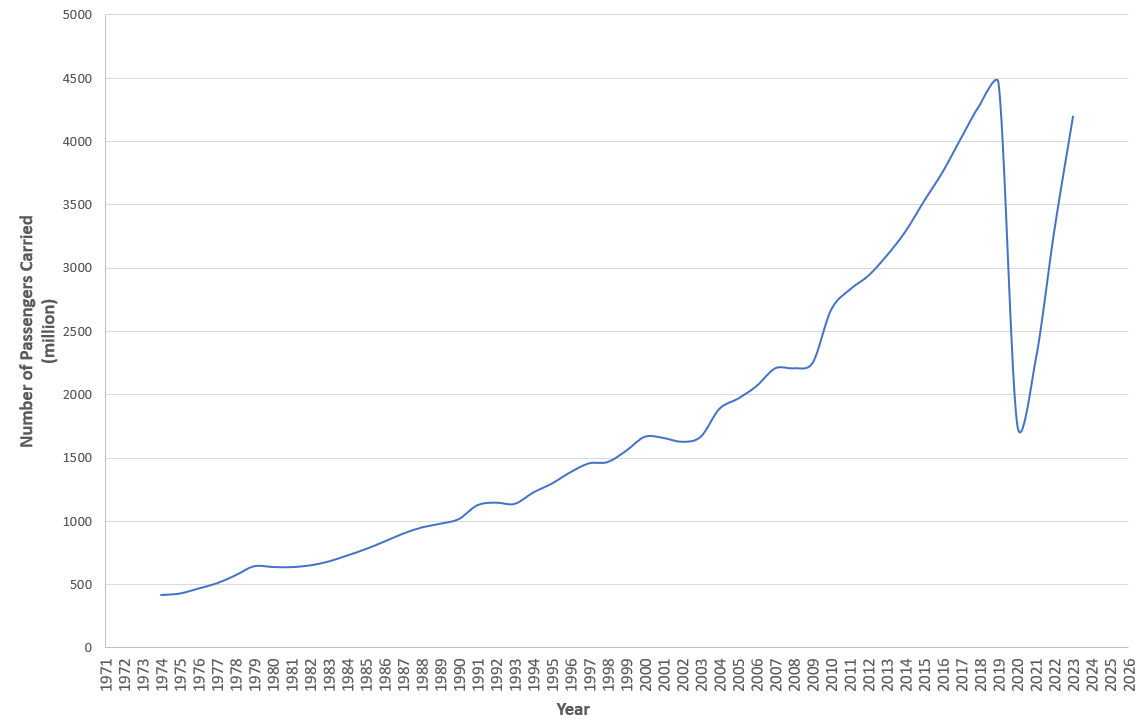
\includegraphics[width=1\linewidth]{Image/passengers.png}
     \end{adjustwidth}
    \caption{World air passenger traffic from 1974 to 2023 \cite{ICAO}}
    \label{fig:air_passengers}
\end{figure}

\noindent Figure \ref{fig:air_passengers} shows a drop in the number of air passengers in 2020. We can explain this drop by the spread of COVID-19 around the world and the introduction of containment measures and travel bans throughout the world. Despite this decrease, the number of passengers started to increase again in the following years, from 2021 onwards. For 2024, certain experts expect a growth in passenger numbers that is likely to even exceed the numbers obtained before COVID-19. That spectacular increase is being accompanied by a considerable increase in the number of flights, thereby generating huge volumes of air traffic. For example, the flight-tracking service Flightradar24 \cite{Flightradar24} indicates that more than 100,000 commercial flights have been operated every day around the world since 2021, as shown in Figure \ref{fig:flights_number}.

\begin{figure}[H]
 \begin{adjustwidth}{-2cm}{}
    \centering
    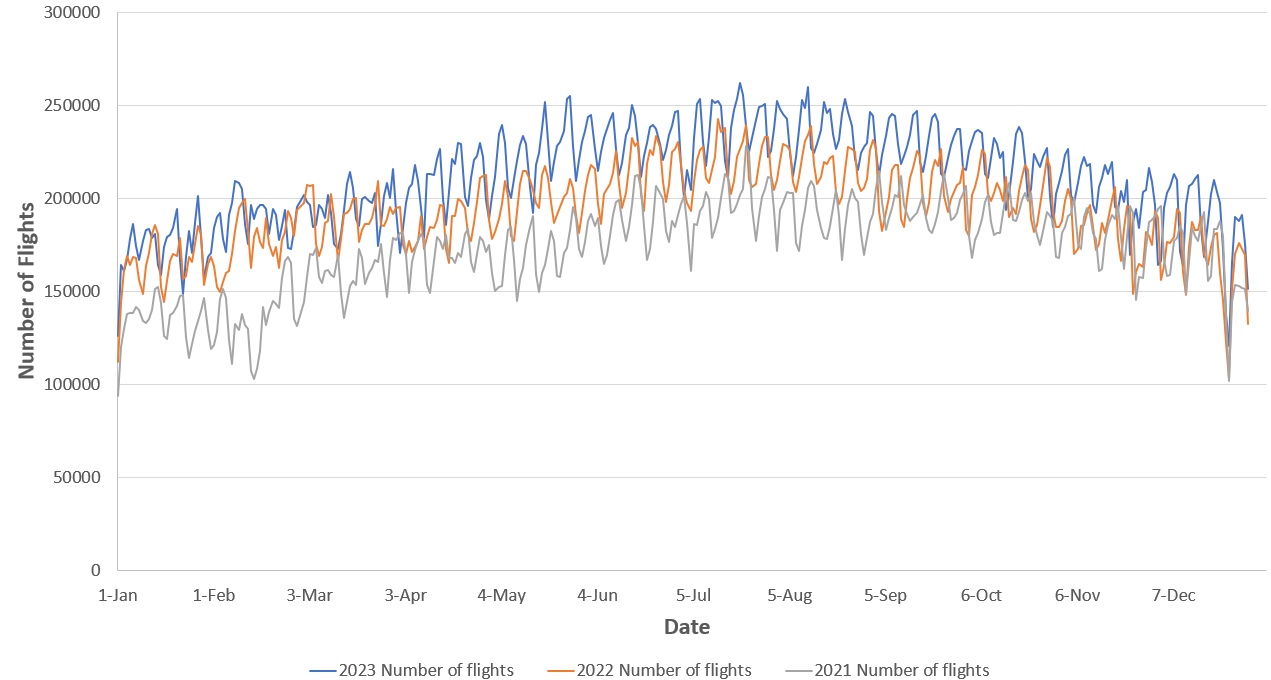
\includegraphics[width=1\linewidth]{Image/flights_number.png}
    \end{adjustwidth}
    \caption{Total number of flights tracked by Flightradar24 from 2021 to 2023 \cite{Flightradar24}}
    \label{fig:flights_number}
\end{figure}

\noindent Figure \ref{fig:flights_number} only takes into account flights tracked by Flightradar24. Thus, this traffic density can make flight management more complex and slightly increase the risk of delays.

\noindent According to the Bureau of Transportation Statistics (BTS) \cite{BTS_flight_delays}, a flight is considered delayed when an aircraft departs or arrives more than 15 minutes later than the scheduled time. Such delays can vary from a few minutes to many hours. In addition, they have a negative impact on airlines, airports and, especially, on the passenger experience. In 2023, airlines faced major difficulties. Indeed, they experienced around 20\% of flights considered delayed according to the BTS data \cite{BTS_flight_delays_statistics}, as shown in Table \ref{tab:flight_bts}.

\begin{longtable}{c c c}
\caption{Flight performance in 2023 \cite{BTS_flight_delays_statistics}}
\label{tab:flight_bts}  \\

\hline
  & \textbf{Number of Operations} & \textbf{\% of Total Operations} \\ \hline
\endfirsthead

\hline
 & \textbf{Number of Operations} & \textbf{\% of Total Operations} \\ \hline
\\
\endhead

\hline \multicolumn{3}{r}{{Continued on next page}} \\ \hline
\endfoot

\hline
\endlastfoot

& & 
\\
On-time
& 5 702 506
& 78.34\%
\\
& & 
\\
Delayed
& 1464537
& 20.12\%
\\
& &
\\
Others (Cancelled or Diverted)
& 111694
& 1.54\%
\\
& &
\\
\end{longtable}

\noindent Moreover, these delays lead to huge additional costs for airlines. According to a report by AirHelp \cite{AirHelp}, the annual costs of flight delays in 2022 are estimated to be between \$26 billion and \$32 billion for the US and between \$20 billion and \$25 billion for Europe, as illustrated in Table \ref{tab:flight_delays_costs}.

\begin{longtable}{c c c}
\caption{Impact of flight delays on the US and Europe economies in US dollars in 2022 \cite{AirHelp}}
\label{tab:flight_delays_costs}  \\

\hline
  & \textbf{USA} & \textbf{Europe} \\ \hline
\endfirsthead

\hline
  & \textbf{USA} & \textbf{Europe}  \\ \hline
\\
\endhead

\hline \multicolumn{3}{r}{{Continued on next page}} \\ \hline
\endfoot

\hline
\endlastfoot

& & 
\\
Airline cost (billion)
& 9-11
& 8-10
\\
& & 
\\
Passenger cost (billion)
& 12-15
& 8-10
\\
& &
\\
Spillover cost (billion)
& 5-6
& 4-5
\\
& &
\\
Total cost (billion)
& 26-32
& 20-25
\\
& &
\\
\end{longtable}
\vspace{0.3cm}
\noindent Such costs include fuel, staff and compensation for the passengers affected \cite{AirHelp}. From the point of view of passengers, such delays cause major inconveniences, including missed connections, the obligation to modify travel plans, and time lost, thus affecting overall satisfaction.

\noindent However, we observe that data imbalance is a recurring problem in predicting flight delays. Indeed, the majority of flights arrive on-time, while a minority experience delays regardless of the year. For example, according to BTS data \cite{BTS_flight_delays_statistics}, an analysis of flight data statistics in 2023 shows that 78.34\% of flights arrive on-time, while 20.12\% of flights are delayed, as shown in Figure \ref{fig:flights_imbalance}.

\begin{figure}[H]
    \centering
    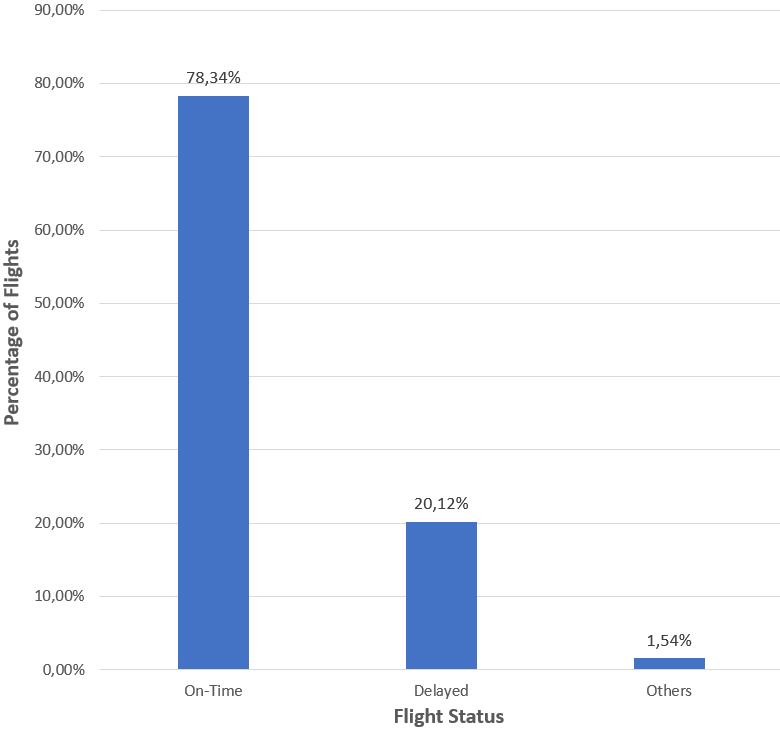
\includegraphics[width=0.8\linewidth]{Image/imbalance.png}
    \caption{Imbalance in historical flight performance data in 2023 \cite{BTS_flight_delays_statistics}}
    \label{fig:flights_imbalance}
\end{figure}

\noindent This large difference in terms of samples between on-time and delayed flights creates a huge imbalance in the flight data. This imbalance can cause a number of difficulties for the prediction models. Indeed, it can make it more difficult for the models to identify any possible patterns in the delayed flights. As a result, the models may be biased. Indeed, they may under-predict delays because they are too influenced by on-time flights. Therefore, it is necessary to use specific techniques which will be explained in detail in the literature review and in the methodology of this thesis.

\noindent With regard to flight delays, they can be divided into many categories \citep{BTS_flight_delays,BTS_flight_delays1}. Below is a list of the different causes of delays: 
\begin{itemize}
    \item \textbf{Air carrier delay \citep{BTS_flight_delays,BTS_flight_delays1}:} Such delays result from internal operational problems such as unplanned aircraft maintenance, staff issues or logistical errors. 
    \item \textbf{Extreme weather delay \citep{BTS_flight_delays,BTS_flight_delays1}:} These delays are due to weather conditions unfavourable to the execution of a flight, such as tornadoes, storms or blizzards.
    \item \textbf{National Aviation System (NAS) delay \citep{BTS_flight_delays,BTS_flight_delays1}:} Such delays are the consequence of operational factors related to the national aviation system. Such factors may include non-extreme weather conditions, airport operations, high traffic volumes and air traffic control.
    \item \textbf{Late-arriving aircraft delay \citep{BTS_flight_delays,BTS_flight_delays1}:} These delays are the result of the late arrival of a previous flight operating with the same aircraft, leading inevitably to the late departure of the current flight.
    \item \textbf{Security delay \citep{BTS_flight_delays,BTS_flight_delays1}:} Such delays may be caused by additional security measures or other security incidents. These include for instance the evacuation of a terminal, the re-boarding of an aircraft because of a security breach or the defective control equipment. 
\end{itemize}

\noindent Besides, Figure \ref{fig:flights_delays} illustrates the distribution of the types of delayed flights for 2023 \cite{BTS_flight_delays_statistics}.

\begin{figure}[H]
    \centering
    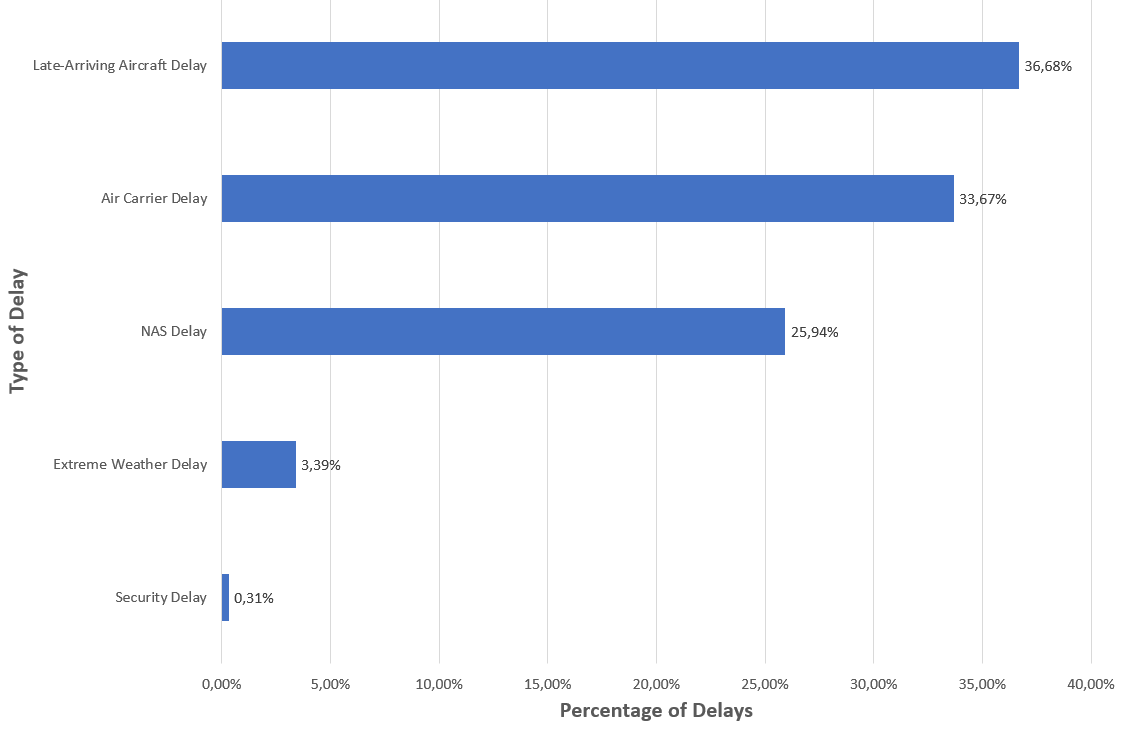
\includegraphics[width=0.89\linewidth]{Image/flight_delays_type.png}
    \caption{Distribution of delayed flight types for 2023 \cite{BTS_flight_delays_statistics}}
    \label{fig:flights_delays}
\end{figure}

\noindent This thesis focuses on weather-impacted flight delays for a number of reasons. Although they account for a smaller percentage, weather delays are critical because of their unpredictability and potential severity. Indeed, weather conditions can lead to important disruptions, which may affect not only individual flights, but also the entire air traffic network. Weather data generally includes information such as temperature, wind speed and direction, precipitation and atmospheric pressure. Nevertheless, it is necessary to recognise the challenge posed by the weather data. Indeed, the reliability of weather data can lead to additional difficulties for prediction models. Weather forecasting is usually prone to uncertainties due to its unpredictable nature \cite{Weather_forecast}. In addition, even with some technological advances of recent years, uncertainty remains in the weather data, albeit to a lesser extent. Such uncertainty can affect the accuracy of flight delay prediction models. Thus, when analysing the results obtained by the various models, this observation must be taken into account. The uncertainty of one-day forecasts is around 2-4\% \cite{Weather_forecast}. This uncertainty rises to 10\% for three-day forecasts and increases further for long-term forecasts \cite{Weather_forecast}.

\section{Motivations}

\noindent The motivations behind the prediction of flight delays are multiple and influenced by different factors. These include economic, environmental, operational, and customer experience aspects. The complete overview of the main drivers outlines the need to undertake the prediction of weather-impacted flight delays.

\noindent One of the major motivations for predicting flight delays is the reduction of costs. Flight delays can result in substantial costs for airline companies, including additional fuel costs, staff costs, passenger compensation and penalties for missed slots \cite{Anupkumar}. For example, the Federal Aviation Administration (FAA) estimated the annual cost of delays at \$33 billion in 2019 \cite{delay_costs}. Thus, it is primordial to accurately predict flight delays. Indeed, by anticipating these delays, the airlines can plan better and reduce any unexpected costs.

\noindent Predicting flight delays helps to improve environmental sustainability. We know that aircraft on the ground or waiting on runways consume fuel unnecessarily, which increases emissions of CO2 and some other pollutants \cite{motivation_environment}. In this way, the precise prediction of flight delays could make it possible to reduce these unnecessary emissions and consumption. Moreover, it is extremely important at a time when the aviation industry is continually looking for ways to considerably reduce its carbon footprint and comply with much stricter environmental regulations \cite{motivation_environment}.

\noindent Moreover, the prediction of flight delays can considerably improve resource management. This potential improvement can be materialised through better optimisation of flight schedules and enhanced air traffic control, resulting in more efficient operations \citep{MAmdouh,Hatipoglu2024}. Such efficiency also guarantees better use of assets and staff. For example, based on forecasts, airlines can adjust their staff assignments to avoid any overwork or underemployment of crews. In addition, the airports can better handle their runways and boarding gates, thereby improving the fluidity of operations.

\noindent Finally, the improvement of the passenger experience is another motivation for predicting flight delays. This enhancement of passenger satisfaction is indispensable, especially in a competitive market. Flight delays can cause considerable inconvenience. These include missed connections, prolonged waiting times and uncertainty about arrival at destination. By predicting and communicating these delays effectively, airlines can keep their passengers informed in real time. This can enable the passengers to change their flight or maybe reorganise their travel plans \citep{Song2020,Efthymiou2019}. In addition, it helps airlines to make the travel experience more fluid and to strengthen customer loyalty.

\noindent Overall, flight delay prediction meets key strategic and operational needs for airlines, ranging from cost reduction to improved passenger satisfaction. These motivations are interconnected and collectively contribute to the general improvement of the airline industry.

\section{Aim \& Objectives}

\noindent The aim of this project is to develop a Deep Learning (DL) model capable of predicting weather-impacted flight delays. By using advanced approaches in both data processing and modelling, this thesis seeks to offer predictions that are as accurate as possible and better than the results achieved from previous research on this topic. To accomplish this aim, several objectives need to be fulfilled. These are listed below: 

\begin{itemize}
    \item  Perform a comprehensive literature review and collect the datasets necessary for the prediction of weather-related flight delays;
    \item Clean and prepare data using several methods from numerous previous research, guaranteeing data quality and feature transformation for the analysis;
    \item Perform Exploratory Data Analysis (EDA) to identify some patterns affecting weather-impacted flight delays and implement a DL model via the feature selection, model architecture design and model training;
    \item Evaluate and validate the implemented model by using performance metrics to guarantee its accuracy and robustness;
    \item Compare the model developed with other existing methods to outline both its advantages and limitations;
\end{itemize}

\section{Contributions}

\noindent The principal contribution of this thesis resides in the implementation of a recently developed DL model, namely the Liquid Neural Network (LNN). This model has never been used previously for predicting flight delays. In addition, this thesis introduces a distinction between weather-related delays and other types of delays. This enables a more targeted analysis of the specific factors affecting each category of delay. Moreover, in this study, advanced methods are adopted, for example, to address imbalances in the flight data. As a result, it ensures that the model can effectively handle minority classes and deliver more robust predictions. Overall, the approach adopted in this thesis provides a new perspective on flight delay analysis and predictions.

\section{Thesis Structure}

%XXX more elaborate

\noindent This thesis is composed of five chapters centered on the prediction of weather-impacted flight delays using DL techniques. In Chapter 1, we discuss the general context of flight delays, outlining their huge increase in recent years and the associated challenges in predicting them. In addition, we cover the main motivations for this thesis, as well as its aim and objectives. This chapter provides a solid foundation and the necessary knowledge to undertake an in-depth analysis in the following chapters.

\noindent Chapter 2 is dedicated to the literature review. It delivers an overview of previous research carried out in recent years on the prediction of flight delays. These studies investigated some approaches using Machine Learning (ML) or DL, proposing advancements in this topic. Moreover, we looked in detail at several DL models, describing their advantages and disadvantages, which will later be used in this thesis. This chapter gives a better understanding of the approaches adopted and some potential improvements to contribute to flight delay prediction.

\noindent For this thesis, Chapter 3 discusses the methodology adopted to predict weather-related flight delays. Building on the literature review in the previous chapter, the methodology is based on an elaborate approach involving data collection, data preprocessing and the application of sampling techniques to deal with data imbalance. In addition, this chapter defines the architecture of the DL models used. Moreover, we explain the performance metrics used to evaluate model performance. This chapter on the detailed methodology forms the basis for the experiments and analyses presented in the following chapter.

\noindent Chapter 4 covers the results and discussions of this thesis. This chapter introduces the EDA, which identified patterns relevant to the prediction of weather-impacted flight delays. Such analysis provides important insights to better understand the data collected and guide the development of prediction models. Subsequently, we present the performance achieved for the different DL models implemented. This chapter also includes a detailed comparison between these models, identifying the one delivering the best performance for predicting weather-related flight delays. In addition, we compared our best model with those from previous research. This chapter offers a constructive critique of the advantages and potential limitations of the models used in this thesis.

\noindent Chapter 5 concludes this thesis and proposes areas for future work. This chapter summarises all the work carried out, from the literature review to the evaluation of DL models for predicting flight delays due to weather conditions. It also delivers a critical analysis of the models adopted. In addition, we discuss ways of improving the performance of predictions of weather delays in the future. These include the use of new models or the extension of this approach to other types of flight delays. This chapter allows us to determine whether the thesis has contributed to any meaningful advancements in the prediction of flight delays.

\chapter{Literature Review}

\section{Related Work}
\label{related_work}
\noindent For decades, we have been noticing a major problem in the aviation industry. Flight delays have a negative impact on airline operations and customer satisfaction. Moreover, these delays are costing airlines in the order of billions. As a result, researchers have focused on developing ways of accurately predicting flight delays. However, they have regularly encountered difficulties with these flight delay predictions. Nevertheless, the latest published studies show that a trend is emerging in flight delay prediction. Indeed, many researchers have applied and used ML or DL techniques/approaches to obtain better results in terms of performance.

\noindent To investigate the importance of weather data in prediction, S. Choi et al. \cite{choi} developed ML/DL models by training and evaluating them with and without weather data. The authors collected data from the US BTS to obtain historical flight performance data. They also collected weather data from the National Oceanic and Atmospheric Administration (NOAA). The methodology used to preprocess the data is quite classic. First, cancelled or diverted flights were considered as delayed flights. Then, for the data selection, they kept only the most important and useful variables for the flight delay prediction. They apply the linear interpolation method to deal effectively with missing data. To ensure that the models performed well, they encoded the categorical variables into numerical variables. Finally, the authors normalised the variables to prevent the models from being dominated by any feature. The authors implemented the following models: Decision Tree (DT), Random Forest (RF), AdaBoost and K-Neighrest Neighbour (KNN). To optimise the hyperparameters of the models, they applied the trial-and-error method. Finally, to reduce the risk of overfitting, the authors applied the 10-fold cross-validation technique. The results showed that integrating weather data during the training and the evaluation of the models greatly improved their performance. This observation was also confirmed by another study carried out by N. Etani \cite{Etani}. Indeed, even though a different methodology was used, the results obtained showed the same trend. These results also showed that the models using weather data achieved better results in terms of performance, particularly the one based on the RF algorithm.

\noindent The importance attributed to weather data has been taken up by other researchers in this field. By integrating weather data, they attempted to improve the accuracy of flight delay predictions. However, despite the clear imbalance in the data used, some researchers have not taken any serious steps to address this problem. V. Sujay et al. \cite{Sujay} implemented the RF, Gradient Boosting and Support Vector Machine (SVM) models. They used a common methodology. They handled missing data with interpolation for categorical variables and mean imputation for numerical variables. They encoded the categorical variables into numerical variables. They normalised the features. To optimise the hyperparameters, the authors employed the grid search, the Random Search and the Bayesian Search algorithms. In addition, to improve the reliability of the models, they applied the cross-validation method. They authors obtained very good results. Indeed, the proposed model achieved at least 92\% for all performance metrics, namely accuracy, precision, recall, and F1-score. In this way, the authors proposed a method capable of easily classifying flight delays from on-time flights. D. Mavris et al. \cite{Mavris} adopted a two-stage methodology based on Recurrent Neural Network (RNN) with Long Short-Term Memory (LSTM) architectures. The first stage predicts the day-to-day delay status of the airport using historical flight performance and weather data for ten major US airports. The second stage refines these predictions for each individual flight delay by combining the day-to-day delay status predictions with flight performance and weather data, using a fully connected multi-layer neural network. Some regularisation techniques such as Dropout are employed to reduce the overfitting. Moreover, the models are trained with the stochastic gradient descent and the mini-batch algorithms. The authors showed that deep models achieved accuracies of 80.63\% and 90.95\% for sequences of 7 and 9 days respectively. These results outperform those of the simple models. For individual delays, a multilayer network achieved an accuracy of 87.42\%. In addition, the authors succeeded in obtaining a model trained on one airport that could be generalised with an accuracy of over 85\% for all but one of the other airports.

\noindent Looking at another key aspect of flight delay prediction, it is important to study the impact of data imbalance on the accuracy of the prediction. The researchers explored different techniques for dealing with data imbalance to identify whether these approaches enhance the prediction results. Choi et al. \cite{choi} developed the RF, AdaBoost, and KNN models. Moreover, in order to deal with data imbalances, they applied the Synthetic Minority Over-sampling Technique (SMOTE) and Random Under-Sampling (RUS) techniques. They found that the application of these sampling techniques slightly decreased the global accuracy for each model. Nevertheless, the number of correctly predicted samples in the case of flight delays has increased, while the number of correctly predicted samples in the case of on-time flights has decreased slightly, but still remained acceptable. They concluded that the use of these techniques improves the identification of flight delays while at the same time providing appropriate performance for the on-time flight classification.

\noindent Therefore, the researchers used weather data and applied different techniques in order to deal with data imbalances. Utilising a combination of these approaches, they intend to improve the accuracy of flight delay predictions. This demonstrates the need to use more advanced data processing methods to try to get more reliable results. Several researchers have used a classic methodology. Indeed, all these researchers encoded their categorical variables into numerical variables, for example using one-hot encoding \cite{kim}. They also normalised their variables. They handled missing values by using one of the following techniques: linear interpolation \citep{choi} or removing rows containing missing values \cite{Tang}, as they represented less than 1\% of the entire dataset. The features were selected according to their importance in predicting flight delays, using for example the Pearson coefficients \cite{hendrickx}. To deal with data imbalances, researchers chose to use SMOTE \citep{hendrickx,choi}, RUS \cite{kim,choi} or weighted metrics \cite{Tang}. To optimise the hyperparameters, they employed grid search \citep{hendrickx,kim}. In addition, to improve the reliability of the models, some researchers applied the cross-validation method \citep{hendrickx,choi}. R. Hendrickx et al. \cite{hendrickx} implemented the RF and MultiLayer Perceptron (MLP) models. They obtained relatively correct results for departure and arrival delays with both MLP and RF models. However, it was noted that while the precision for both models had a rather interesting score, the F1-scores were very poor. Furthermore, the authors demonstrated the possible influence of imbalance ratios for SMOTE or RUS.  Y. Tang \cite{Tang} developed the DT, RF, KNN, SVM, Gradient Boosted Tree, Gaussian Naive Bayes, and Logistic Regression models. He obtained excellent results. Indeed, the DT model achieved the best performance with an accuracy of 0.9778, a precision of 0.9777, a recall of 0.9778, and an F1-score of 97.78\%. The RF and Gradient Boosted Tree models also had interesting results. However, the performance of the KNN was significantly lower than the other models.

\noindent Furthermore, some researchers found it interesting to train and evaluate the models by collecting weather data at different intervals relative to the flight departure time. Indeed, S. Kim and E. Park \cite{kim} collected weather data at intervals of 2h, 4h, 8h, 16h, 24h, and 48h before the flight departure. They used the DT, RF, SVM, KNN, Logistic Regression, Extreme Gradient Boosting (XGB) and LSTM models. They obtained acceptable results for the RF, DT, and LSTM models. Indeed, these models outperformed the others in terms of performance. Additionally, they observed that the performance of the models depends on the time interval of the weather data before departure used. As the interval increases, the performance of the models decreases. Choi et al. \cite{choi} collected weather data at the following intervals before the flight departure: 0 days, 1 day, and 5 days. They implemented the RF, AdaBoost, and KNN models. They had interesting results for the RF model with 80.36\% accuracy and the AdaBoost model with 71.43\%. However, these two models struggled to predict the delay class. Additionally, the KNN model delivered very poor results with an accuracy of 35.71\%. Similar to the previous research, they noted the influence of the time interval for collecting weather data before departure on model performance. Indeed, when the time interval increases, the global accuracy decreases. For instance, the accuracy for 0 days was 80.36\%, but the accuracy for 5 days fell to 26.79\%.

\setlength\LTleft{-1cm}
\begin{longtable}{>{\raggedright\arraybackslash}p{2.5cm} p{6.5cm} >{\raggedright\arraybackslash}p{5.6cm} >{\centering\arraybackslash}p{2.5cm}}
\caption{Summary of previous research on flight delay prediction (1/2} \label{tab:summary_previous1}  \\

\hline
\textbf{Authors}  & \textbf{Methods} & \textbf{Datasets} & \textbf{Data Period} \\ \hline
\endfirsthead

\hline
\textbf{Authors}  & \textbf{Methods} & \textbf{Datasets} & \textbf{Data Period} \\ \hline
\\
\endhead

\hline \multicolumn{4}{r}{{Continued on next page}} \\ \hline
\endfoot

\hline
\endlastfoot

& & &
\\
N. Etani \cite{Etani}
& Models: RF, Gradient Boosting, SVM, DT, AdaBoost\newline Imbalance: Balanced parameter set to class weight parameter
& Flight: FLIGHTSTATS database\newline Weather: Japan Meteorological Agency
& 1 Mar 2012\newline -\newline 3 Dec.2018
\\
& & &
\\
V.Sujay et al. \cite{Sujay}
& Models: RF, Gradient Boosting, SVM\newline Imbalance: None
& Flight ant Weather: APIs and databases
& Unknown
\\
& & &
\\
D. Mavris et al. \cite{Mavris}
& Models: RNN with LSTM architectures\newline Imbalance: None
& Flight and weather: ten major US airports
& Jan. 2010\newline -\newline Aug. 2015
\\
& & &
\\
R. Hendrickx et al. \cite{hendrickx}  
& Models: RF, MLP \newline Imbalance: SMOTE, RUS
& Flight: Amsterdam Airport Schiphol\newline Weather: METAR 
& 2015 - 2018 
\\
& & &
\\
Y. Tang \cite{Tang}
& Models: DT, RF, KNN, SVM, Gradient Boosted Tree, Gaussian Naive Bayes, Logistic regression\newline Imbalance: Weighted performance metrics
& Flight: BTS\newline Weather: Weather Underground
& Nov. 2019 \newline -\newline Dec. 2020
\\
& & &
\\
S. Choi et al. \cite{choi}  
& Models: DT, RF, AdaBoost, KNN\newline Imbalance: SMOTE, RUS 
& Flight: BTS\newline Weather: NOAA   
& 2005 - 2015
\\
& & &
\\
S. Kim and E. Park \cite{kim}
& Models: DT, XGB, SVM, KNN, Logistic Regression, RF, LSTM\newline Imbalance: RUS
& Flight: Incheon Airport, BTS\newline Weather: Korean Meteorological Administration, Weather Underground
& 2010 - 2021
\\
& & &
\\ 

\end{longtable}

\setlength\LTleft{-1cm}
\begin{longtable}{>{\raggedright\arraybackslash}p{2.5cm} p{7.3cm} >{\raggedright\arraybackslash}p{7.3cm}}
\caption{Summary of previous research on flight delay prediction (2/2)} \label{tab:summary_previous2} \\

\hline
\textbf{Authors}  & \textbf{Results} & \textbf{Gaps}\\ \hline
\endfirsthead

\hline
\textbf{Authors}  & \textbf{Results} & \textbf{Gaps}\\ \hline
\\
\endhead

\hline \multicolumn{3}{r}{{Continued on next page}} \\ \hline
\endfoot

\hline
\endlastfoot

& & 
\\
N. Etani \cite{Etani}
& - Predictive models based on weather data proved superior to those without weather data
\newline - RF with weather data showed the best overall performance with high precision, recall and F1-score, especially for on-time arrival predictions
\newline - The learning period plays a major role in the performance of the models, with longer learning periods producing better results
& - Difficulties of models in capturing the complex factors influencing delays
\newline - Models have a tendency to overfit
\newline - Global accuracy obtained by the models remains relatively low compared to other studies
\\
& & 
\\
V.Sujay et al. \cite{Sujay}
& - The proposed system achieves 95\% accuracy
\newline  The proposed system correctly identified 5500 on-time flights and 4700 delayed flights, with just 500 misclassified on-time flights and 300 wrongly predicted delayed flights
& - Adaptability of the proposed system to deal with real-time data and its deployment in different airline environments
\newline - Reliance on historical data and sensitivity to changes in the aviation environment
\\
& & 
\\
D. Mavris et al. \cite{Mavris}
& - Day-to-day delay status models: around 78\% accuracy for a delay threshold of 15min and around 90\% accuracy for a delay threshold of 30min
\newline - Individual flight delay models: high accuracy ranging from 85,32\% to 87,42\%
\newline - Accuracy of day-to-day model for different airports ranging from 71.34\% to 91.81\%
& - Increased complexity of deep RNNs, leading to convergence issues
\newline - Less accurate predictions for lower delay thresholds
\newline - Variability in model performance across different airports
\newline - Requires large amounts of data for optimal performance
\\
& & 
\\
R. Hendrickx et al. \cite{hendrickx}  
& - RF: precision of 66\% for departure delays and 71,3\% for arrival delays
\newline - MLP: precision of 61,4\% for departure delays and 69,2\% for arrival delays
\newline - Sampling techniques improve the performance of the models in terms of F1-score, while reducing false positives 
& - No validation of the model trained on one airport on others to ensure generalisability 
\newline -  Need to explore other ML algorithms to validate the approach
\newline - Difficulty in integrating these predictive models into existing airport management systems due to accuracy below 80\%
\\
& & 
\\
Y. Tang \cite{Tang}
& - DT model showed the best performance of the seven algorithms tested, with accuracy, precision, recall and F1-score close to 97\%
\newline - Tree-based ensemble classifiers tend to perform better than other basic models

& - No use of sampling techniques such as SMOTE, which can improve model performance
\newline - Data is limited to a single year, and extending the dataset to a longer period would make it possible to obtain a more robust model
\\
& & 
\\
S. Choi et al. \cite{choi}  
& - RF model showed the best performance with an accuracy of 80,36\% and an AUC of 0.68
\newline - Using SMOTE improves the identification of delayed flights despite a drop in global accuracy
\newline - Integrating weather data considerably improves the accuracy of predictions compared to simply relying on flight data
& - The performance of the models are influenced by the uncertainty of the weather forecasts
\newline- Imbalanced data remains a challenge for accurate prediction even with the use of SMOTE/RUS
\newline - Classifiers have a tendency to overfit, particularly for KNN and DT models
\newline - Models do not take into account delays caused by non-weather factors, which impacts the accuracy of delay prediction
\\
& & 
\\
S. Kim and E. Park \cite{kim}
& - High accuracy in short-term predictions for the optimal models of each airport: 74.9\% accuracy for the Incheon model, 85.2\% accuracy for the JFK model and 78.5\% accuracy for the MDW model in 2-hour forecasts.
\newline -  LSTM models outperform the other models in most of the evaluation measures for JFK and MDW
\newline - Random Forest model showed the highest accuracy for ICN
& - Limited generalisation of results due to regional and national variability in weather conditions
\newline - Inferior performance related to missing feature for Incheon airport model
\\
& & 
\\ 

\end{longtable}

\noindent In this work, we aim to implement a recently developed DL method that has not yet been applied to flight delay prediction. We intend to carry out an in-depth study and analysis of the reliability of this innovative model in terms of prediction performance. In addition, the use of this model could potentially deliver solutions to the gaps identified in previous research, as discussed in Table \ref{tab:summary_previous2}. Therefore, a thorough comparison is performed by comparing the developed model with several DL models adopted in previous studies.

\section{Liquid Neural Networks}

\noindent In the area of artificial intelligence (AI), Neural Networks (NNs) are frequently utilised for solving very complex problems \cite{Sajid}. The principles of these ML algorithms are based on imitating the structure and operational capabilities of the human brain \cite{Sajid}. However, these networks have many drawbacks, such as their inability to deal with data in real-time \cite{Sajid}. Consequently, over the past few years researchers have been exploring innovative ways of enhancing the performance of these NNs and overcoming a number of their limitations. Thus, a group of researchers at MIT has introduced a new approach called Liquid Neural Network (LNN) \cite{Sajid}.

\subsection{Fundamental Concepts}

\noindent LNNs are a type of RNN characterised as being continuous in time \citep{Boesch,Keary,Sajid}. These networks are able to process time-series data and are also capable of adapting to changing environments. As they are inspired by the dynamic behaviour of liquids, LNNs are built following a dynamic architecture \cite{Tyagi}. Indeed, in contrast to traditional NNs where weights and connections are fixed, LNNs present weights and connections that can vary depending on the current and past input \cite{Keary}. This structure is inspired by the nervous system of a microscopic worm, which has only 302 neurons but manages to present dynamic and complex behaviour \citep{Boesch,Sajid}.

\subsection{Advantages and limitations}

\noindent LNNs present many advantages. These neural networks are highly adaptable \citep{Tyagi,Keary}. Indeed, they are able to adjust to changes in input data. This characteristic makes these networks particularly useful for real-time applications. Moreover, LNNs show major improvements in robustness compared with classic NNs \citep{Tyagi,Keary}. LNNs provide a better management of disturbances and noise in the data. Indeed,their dynamic architecture ensures that these networks concentrate only on relevant information. Finally, LNNs need less computational resources than traditional NNs \cite{Keary}. This can be explained by the dynamic architecture of the LNNs, which require a smaller number of neurons.

\noindent However, LNNs also present a number of limitations. LNNs have some difficulties in dealing with static or fixed data, in contrast to classic NNs \citep{Keary,Boesch}. In addition, LNNs have some problems in reaching the optimum weights during the training because of the vanishing gradient problem \citep{Keary,Boesch,Sajid}. Therefore, it is very difficult to ensure the stability and convergence of these LNNs. This limits their capacity to learn long-term dependencies. Finally, the tuning of LNNs parameters can be complex \citep{Keary,Boesch,Sajid}. Indeed, it can be costly and time consuming. In addition, if the settings are not made properly, the LNNs are unlikely to perform as well as they should.

\subsection{Applications}

\noindent LNNs can be applied in many areas because of their ability to deal with time series data. They can be utilised in the medical sector \cite{Boesch} to make diagnoses by using medical images. Indeed, LNNs are appropriate for some image processing tasks, such as object tracking and object recognition. Moreover, LNNs can be utilised for autonomous drones \citep{Boesch,Keary}. Indeed, a recent study by MIT researchers shows that LNNs offer better results in terms of performance than other NNs in this sector. LNNs enable the drones to navigate more efficiently in unknown areas. LNNs can also be applied to self-driving cars \citep{Boesch,Keary}. Employing LNNs rather than other AI models can be very beneficial because LNNs have the ability to adapt to new scenarios that are not included in their training data. They can therefore make these cars more reliable and also reduce the risk of accidents. Finally, LNNs can be used for natural language processing (NLP) \citep{Boesch,Sajid}. Classic DL models typically use a large training datasets for NLP tasks such as sentiment analysis and machine translation, which can be very time consuming. As a result, the use of LNNs in NLP can significantly reduce the computational costs.

\section{Long Short Term Memory}

\subsection{Fundamental Concepts}

\noindent LSTMs, introduced by Hochreiter and Schmidhuber in 1997, are an extended form of RNNs designed for processing sequential data \citep{LSTM1,LSTM2}. The principle of such networks is their capacity to store information easily over a long period of time \cite{LSTM1}. Indeed, they are also able to process long-term dependencies through their unique memory cell architecture \cite{LSTM1}. This architecture has three gates \citep{LSTM1,LSTM2}:
\begin{itemize}
    \item Input gate: controls the entry of new information into the memory cell.
    \item Forget gate: identifies which information in the memory cell is removed. 
    \item Output gate: regulates the flow of information out of the memory cell. 
\end{itemize}
 
\noindent All these gates control together the flow of data into memory cells. As a result, over long sequences, it is possible for LSTMs to selectively keep or forget information.

\subsection{Advantages and limitations}

\noindent LSTMs deliver a number of interesting advantages compared with classic RNNs. Indeed, LSTMs can deal with long and complex data sequences by employing their gate functions to keep useful information and eliminate irrelevant details \cite{LSTM3}. In addition, LSTMs considerably improve both learning stability and performance. This is reflected in the vast reduction of the vanishing and exploding gradient problems encountered by classic RNNs \cite{LSTM3}. Besides, LSTMs are versatile, as they are highly adapted to a wide range of applications necessitating sequential data processing .

\noindent However, LSTMs also have some major limitations. Their architecture consumes more computational and memory resources than conventional RNNs \cite{LSTM3}. Besides, the training of LSTM models can be quite intensive in terms of computation, leading frequently to the use of large datasets and to a longer training time \cite{LSTM3}. The complexity of LSTM models can make them really difficult to interpret and understand. This can lead to problems of model transparency \cite{LSTM3}.

\subsection{Applications}

\noindent LSTMs can be employed in many areas because of their capacity to deal with temporal data sequences. They are especially useful for speech-related tasks \cite{LSTM1}. Indeed, LSTMs achieve good performance in speech transcription and recognition \cite{LSTM1}. They are able to recognise speech patterns and transcribe them into text. Moreover, they can be utilised for several video processing tasks such as object detection \cite{LSTM1}. Indeed, the architecture of LSTMs is quite adapted for analysing video and extracting any relevant information. LSTMs are also employed for time series forecasting tasks such as weather prediction, as they have the ability to identify some patterns in this type of data \cite{LSTM1}.

\section{MultiLayer Perceptron}

\subsection{Fundamental Concepts}

\noindent MLPs are a type of feedforward neural network developed in the 1960s. Such NNs were designed based on the structure of the human brain \cite{MLP2}. Moreover, in this network, all the nodes are interconnected with nodes in other layers \citep{MLP1,MLP2,MLP3}. The architecture of MLPs is composed of three types of layers: 
\begin{itemize}
    \item Input layer \citep{MLP1,MLP3}: This layer receives the input signals and sends them to the hidden layers.
    \item Hidden layers \citep{MLP1,MLP3}: One or many hidden layers process the information received from the input layer. Besides, the number of hidden layers depends on the specific task. In addition, each neuron present in the hidden layers employs a non-linear activation function, such as the Rectified Linear Unit (ReLU) function. 
    \item Output layer \citep{MLP1,MLP3}: This layer returns the final result of the model. The number of nodes in this layer is set according to the type of problem.
\end{itemize}
 
\noindent The principle of MLP is based on the backpropagation algorithm \cite{MLP1}. The major objective of this algorithm is to adjust the weights of the connections between neurons \citep{MLP1,MLP3}. It will help to considerably minimise the errors in the prediction of the model \citep{MLP1,MLP3}.

\subsection{Advantages and limitations}

\noindent MLPs have some major advantages. They are well suited to the processing of non-linear problems \cite{MLP3}. In addition, these models are highly versatile, as they can be utilised for a large range of tasks \cite{MLP1}. MLPs can deal with high-dimensional data \cite{MLP3}. They are therefore able to solve some complex problems. Since MLPs are robust to noise, they can deal easily with missing values.

\noindent However, MLPs also present many limitations. The training of MLPs can necessitate important computational resources, in particular with deep architectures and large amounts of data \cite{MLP3}. Besides, MLP models are strongly susceptible to overfitting on the training data \cite{MLP1}. Indeed, if the structure of the model is too complex, it may fail to generalise on the unseen data. Finally, it can be difficult to interpret the predictions of MLPs due to their complex architecture \cite{MLP1}.

\subsection{Applications}

\noindent MLPs are used in many areas thanks to their capacity to determine numerous complex relationships between data. They can notably be utilised in image processing tasks such as image recognition, although they are not the best model for this task \cite{MLP4}. They can also be employed for time series forecasting to predict financial trends or weather conditions by identifying complex trends \cite{MLP4}. Finally, they are also suitable for NLP tasks. Indeed, MLPs are efficient in character recognition and can present some interesting results in tasks such as sentiment analysis or machine translation \cite{MLP4}.

\chapter{Methodology}

\noindent As previously stated, the objective of this thesis is to develop DL models capable of predicting weather impacted flight delays. To address this problem, we followed a rigorous methodology illustrated in Figure \ref{fig:proposed_methodology}. This methodology includes a number of key steps, from problem definition, data collection and preprocessing to the evaluation of the prediction models.

\begin{figure}[H]
    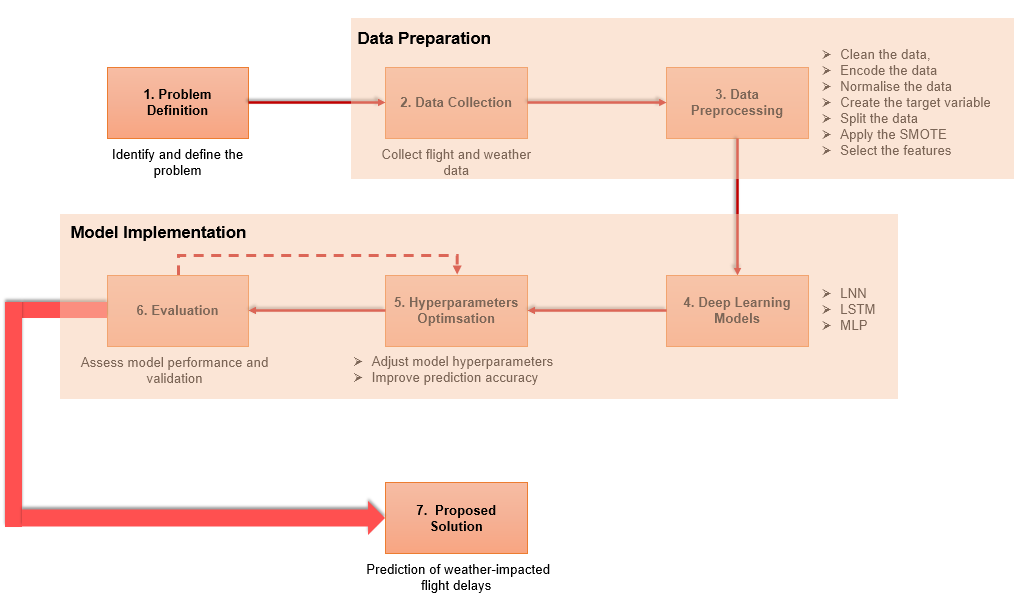
\includegraphics[width=1.03\linewidth]{Image/methodology.png}
    \caption{Diagram of the proposed methodology}
    \label{fig:proposed_methodology}
\end{figure}

\section{Problem Definition}
\label{problem_definition}

\noindent The prediction of flight delays caused by weather conditions is a very complex and critical task in the aviation industry, particularly for airline companies. To address this problem, we adopted a multiclass classification approach, where the idea is to predict three distinct classes, as discussed when creating the target variable in section \ref{target_variable}.

\noindent In addition, it is important to separate delays caused by weather conditions from those due to other factors. Indeed, this can improve the chances of obtaining more accurate predictions. Moreover, this distinction enables specific solutions to be adapted to each type of delay. However, this problem raises many challenges. One is the issue of data imbalance, as flight delays are often much less frequent than on-time flights. Next, preprocessing and feature selection are important to ensure that the data utilised are both of high quality and relevant. Finally, the evaluation of DL models needs rigorous criteria to guarantee that the models are both accurate and robust.

\noindent By defining the problem in this way, this thesis focuses on developing accurate and robust models for predicting flight delays. We took into account the data complexities inherent in the nature of delays and the features.

\section{Data Collection}
\label{data_collection}

\noindent To carry out this thesis on the prediction of flight delays due to weather conditions, we collected data from two main sources: BTS and Weather Underground. The collection period covers 2010 to 2023, excluding 2019 and 2020. Indeed, these two years were excluded from the analysis due to the exceptional disruptions caused by the COVID-19 pandemic. We utilised these two sources because of their reliability and relevance, as demonstrated by a previous study \cite{kim}. In addition, we limited our study to data from a single airport, as delay conditions can differ depending on geographical location. Below are the complete details of the data collection process.

\noindent We obtained flight data for the JFK airport from the BTS website \cite{bts_datacollection}. Indeed, the US BTS is a source renowned for the reliability and accuracy of its statistics on commercial flights. This data was extracted and stored in a Pandas dataframe for further analysis. Table \ref{tab:flight_data_features} lists all the features extracted.

% XXX add type (Done)
% XXX crescent (Done)
\setlength\LTleft{-1.8cm}
\begin{longtable}{l p{5cm} c >{\centering\arraybackslash}p{4cm} }
\caption{List of Flight data features} \label{tab:flight_data_features} \\

\hline
\textbf{Features} & \textbf{Descriptions} & \textbf{Attribute Type} & \textbf{Examples} \\ \hline
\endfirsthead

\hline
\textbf{Features} & \textbf{Descriptions} & \textbf{Attribute Type} & \textbf{Examples} \\ \hline
\endhead

\hline \multicolumn{4}{r}{{Continued on next page}} \\ \hline
\endfoot

\hline
\endlastfoot

FL\_DATE & The flight date & DateTime & 1/1/2010 12:00:00 AM \\ 
OP\_UNIQUE\_CARRIER & The unique code of the carrier & Categorical (nominal) & AA \\ 
TAIL\_NUM & The tail number & Categorical (nominal) & N319AA \\ \
OP\_CARRIER\_FL\_NUM & The flight number & Numerical (discrete) & 185 \\ 
ORIGIN & The airport of origin & Categorical (nominal) & JFK \\ \
DEST & The airport of destination & Categorical (nominal) & LAX \\ 
CRS\_DEP\_TIME & The scheduled departure time & Numerical (continuous) & 2000 \\ 
DEP\_TIME & The actual departure time & Numerical (continuous) & 1958 \\ \
DEP\_DELAY & The difference in minutes between the scheduled departure time and the actual departure time & Numerical (nominal) & -2.0 \\ \
DEP\_DEL15 & An indicator of whether the flight is delayed on departure & Binary (categorical) & 0.0 \\ 
TAXI\_OUT & The time elapsed between the departure from the boarding gate at the airport of origin and the take-off & Numerical (continuous) & 5.0 \\ 
WHEELS\_OFF & The time at which the aircraft's wheels lift off the ground & Numerical (continuous) & 2003 \\ \
WHEELS\_ON & The time at which the aircraft wheels touch down on the ground & Numerical (continuous) & 2252 \\ \
TAXI\_IN & The time elapsed between the wheels landing and arrival at the boarding gate at the airport of destination & Numerical (continuous) & 8.0 \\ 
CRS\_ARR\_TIME & The scheduled arrival time & Numerical (continuous) & 2240 \\ 
ARR\_TIME & The actual arrival time & Numerical (continuous) & 2300 \\ 
ARR\_DELAY & The difference in minutes between the scheduled arrival time and the actual arrival time & Numerical (continuous) & 20.0 \\ 
ARR\_DEL15 & An indicator of whether the flight is delayed on arrival & Binary (categorical) & 1.0 \\ 
CANCELLED & An indicator of whether the flight has been cancelled & Binary (categorical) & 0.0 \\ 
CANCELLATION\_CODE & An indicator to indicate the reason for cancellation & Categorical (nominal) & B \\ 
DIVERTED & An indicator of whether the flight has been diverted & Binary (categorical) & 0.0 \\ 
CRS\_ELAPSED\_TIME & The expected duration of the flight in minutes & Numerical (continuous) & 160.0 \\ 
ACTUAL\_ELAPSED\_TIME & The actual duration of the flight in minutes & Numerical (continuous) & 182.0 \\ 
AIR\_TIME & The duration of the actual flight, from take-off (WHEELS\_OFF) to landing (WHEELS\_ON) & Numerical (continuous) & 169.0 \\ 
DISTANCE & The distance between the two airports in miles & Numerical (continuous) & 2475.0 \\ 
CARRIER\_DELAY & The carrier delay in minutes & Binary (categorical) & 5.0 \\ 
WEATHER\_DELAY & The weather delay in minutes & Binary (categorical) & 3.0 \\ 
NAS\_DELAY & The National Air System (NAS) delay in minutes & Binary (categorical) & 6.0 \\ 
SECURITY\_DELAY & The security delay in minutes & Binary (categorical) & 2.0 \\ 
LATE\_ARRIVAL\_DELAY & The Late Aircraft delay in minutes & Binary (categorical) & 4.0 \\ 
\end{longtable}

\noindent We collected the weather data from the Weather Underground website \cite{weather_underground}. Indeed, Weather Underground is an online service known for delivering historical weather conditions. To obtain this data, we utilised a web scraping technique for automating the retrieval process. We noted that the weather data is displayed on this website in a table generated dynamically by JavaScript. As a result, we used the Selenium \cite{Selenium} package in Python to automate website navigation and data extraction. The Python script using Selenium was programmed to open the Weather Underground Webpage for the JFK Airport. Once the page is loaded, the script extracts the most important weather information. We also converted the data during extraction into the appropriate units. For example, temperatures in Fahrenheit were converted to Celsius, wind speeds in miles per hour were converted to kilometres per hour, and so on. Moreover, we stored the weather data in a Pandas dataframe. This data is very essential as they deliver a major insight into the possible influence of weather on flight delays. Note that we collected weather data at different time intervals before flight departure, namely: 0 hour, 2 hours, 4 hours, 8 hours, 16 hours, 24 hours and 48 hours, as mentioned in the literature review section \ref{related_work} on related work. Table \ref{tab:weather_data_features} summarises all the features extracted.

\setlength\LTleft{-1cm}
\begin{longtable}{ c p{5cm} c c }
\caption{List of Weather data features} \label{tab:weather_data_features} \\

\hline
\textbf{Features} & \textbf{Descriptions} & \textbf{Attribute Type} & \textbf{Examples} \\ \hline
\endfirsthead

\hline
\textbf{Features} & \textbf{Descriptions} & \textbf{Attribute Type} & \textbf{Examples} \\ \hline
\endhead

\hline \multicolumn{4}{ r }{{Continued on next page}} \\ \hline
\endfoot

\hline
\endlastfoot
DateTime & The flight date & DateTime & 2010-01-01 00:51:00 \\ 
Temperature (°C) & The temperature in Celsius & Numerical (continuous) & 1 \\ 
Dew Point (°C) & Dew point temperature in Celsius & Numerical (continuous) & -1 \\ 
Humidity (\%) & The humidity & Numerical (continuous) & 92 \\ 
Wind & The wind direction & Categorical (nominal) & SW \\ 
Wind Speed (km/h) & The wind speed in km/h & Numerical (continuous) & 14 \\ 
Wind Gust (km/h) & The wind gust in km/h & Numerical (continuous) & 6 \\
Pressure (hPa) & The pressure in hPa & Numerical (continuous) & 1015.58 \\ 
Precip. (mm) & The precipitation in mm & Numerical (continuous) & 0 \\ 
Condition & The weather condition & Categorical (nominal) & Cloudy \\ 

\end{longtable}

\noindent With these two datasets, we obtain a solid database rich in information. Consequently, it will be helpful for us to successfully develop reliable flight delay prediction models.

\section{Data Preprocessing}

\noindent Data preprocessing is an extremely important step, as it guarantees that the data are properly prepared for both model training and evaluation. Indeed, a well-prepared dataset can considerably improve the global performance of the models by producing more precise predictions. The following section covers the different phases of preprocessing, including the management of missing values, the encoding of categorical data, the normalisation of variables and the creation of the target variable. It also covers the division of data into training, validation and test datasets, the use of one sampling technique and the selection of the most important features.

\subsection{Handling missing values}

\noindent Managing missing values in datasets is a crucial step in data preprocessing. Indeed, missing values can lead to bias and errors in prediction models if they are not handled correctly. From the literature review, we see that authors have either replaced or removed missing values in order to keep data integrity. Below is the method adopted to deal with missing values in this thesis:

\begin{enumerate}
    \item We determined the columns and rows containing missing values. In this way, we found that the flight and weather data contained missing values, with the majority of these being present in the flight data.
    \item We removed some columns responsible for many missing values in the flight data. Indeed, the decision to delete these columns was justified by the fact that they were not really necessary for predicting flight delays. As a result, the columns `DIVERTED', `CANCELLED' and `CANCELLATION\_CODE', all taken from the flight data, have been removed.
    \item  We also replaced certain missing values with values that we believed to be consistent. For example, we observed that when the flight was on-time, the columns associated with delays, such as weather delay or security delay, included missing values. As a result, we replaced these missing values with zeros, purely as a matter of logic. Similarly, in other situations where missing values could be replaced by coherent values, we applied this approach.
    \item  Finally, we also deleted some rows containing missing values, as they represented only a very small proportion of the total dataset.
\end{enumerate}

\noindent This proposed method of dealing with missing values allowed us to keep as much data as possible without introducing bias.

\subsection{Data encoding}

\noindent An important step in data preprocessing is the encoding of categorical variables. This step is necessary for the correct use of DL models. Indeed, these models require numerical inputs during both training and prediction phases. In this way, the categorical variables need to be transformed into a format that the models can interpret \cite{Encoding}. From the literature review, we found that authors often utilised encoding techniques such as one-hot encoding. Below is the method adopted to encode categorical variables:

\begin{enumerate}
    \item  We identified all the categorical variables contained in the dataset.
    \item We adopted the following technique for encoding each categorical variable: the label encoding method \cite{LabelEncoding}. This approach involves attributing a unique numerical value for each categorical value. This technique is illustrated in Figure \ref{fig:label_encoding}.

    \begin{figure}[H]
        \centering
        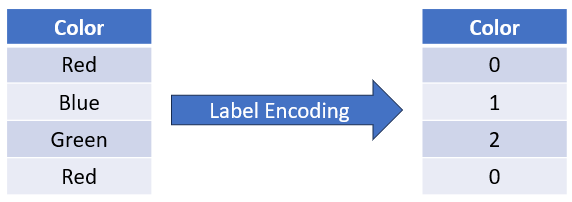
\includegraphics[width=0.75\linewidth]{Image/label_encoding.png}
        \caption{Label Encoding method used on a categorical variable}
        \label{fig:label_encoding}
    \end{figure}
    
    \item We checked that each categorical variable had been correctly encoded.
\end{enumerate}

\noindent It should be noted that we prefer to use the label encoding technique rather than the one-hot encoding method. Indeed, label encoding does not need the creation of new columns. As a result, it helps to keep the dimension of the data and reduce the complexity of the calculations considerably \cite{LabelEncoding}. However, one of the principal limitations of label encoding is the arbitrary order imposed on the data \cite{LabelEncoding}. Therefore, it can lead the model to suppose false relationships.

\subsection{Data normalisation}

\noindent A crucial step in data preprocessing is the normalisation of numerical variables. This step involves scaling the numerical variables to ensure they all have the same range of values between 0 and 1 \cite{Normalisation}. Normalisation is essential because it enables DL models to perform optimally \cite{Normalisation}. Indeed, these models perform best when the input data are on comparable scales. Consequently, given the recurrent presence of data with very different value ranges, we decided to adopt a normalisation technique \cite{Normalisation}. From the literature review, we found that authors often use normalisation techniques such as Min-Max Scaling. Below is the method used to normalise the numerical variables:

\begin{enumerate}
    \item We identified all the numerical variables contained in the dataset.
    \item We applied the Min-Max \cite{MinMax} Scaling technique for each numerical variable. This method is based on the following equation \cite{MinMax}:
    \begin{align}
        x_{\text{scaled}} &= \frac{x - x_{\text{min}}}{x_{\text{max}} - x_{\text{min}}} \label{eq:scaled}
    \end{align}
where x the value of the variable, \(x_{min}\) the minimum value of the variable, \(x_{max}\) the maximum value of the variable and \(x_{scaled}\) the scaled value of the variable.\\

In this way, each variable value is transformed using this normalisation formula \ref{eq:scaled} into the range [0, 1].
    \item We checked that each numerical variable was correctly normalised.
\end{enumerate}

\noindent This proposed data normalisation method guaranteed that each variable had a balanced contribution to model training. As a result, it prevented some variables from dominating the learning process of DL models. Besides, this method helped to keep the optimisation process stable, which enabled faster convergence during gradient-based learning. Consequently, the risks associated with the vanishing or exploding gradients were reduced.

\subsection{Target variable creation}
\label{target_variable}

\noindent Another crucial step in data preprocessing is the creation of the target variable. Indeed, the creation of the target variable is very important for clearly outlining the objective of the model prediction \cite{TargetVariable}. We identified that it is more pertinent to just focus on arrival delays, given the objective of predicting flight delays due to weather conditions. In this way, we can directly capture the possible influence of weather conditions on the ability of aircraft to land on-time. We created a target variable that categorises flights into three classes:
\begin{itemize}
    \item On-time flights (0): Flights that arrive on-time or with a small delay of less than 15 minutes, as established by BTS. 
    \item Flights delayed due to non-weather conditions (1): Delays caused by factors other than extreme weather conditions, such as technical or operational problems. 
    \item Flights delayed due to weather conditions (2): Delays uniquely caused by extreme weather conditions.
\end{itemize}

This classification guarantees that the models are trained consistently, leading to accurate predictions aligned with the expected objectives.

\subsection{Data split}

\noindent Another important step in data preprocessing is data splitting. This involves separating the data into different sets to train, validate and test the models. Moreover, this method ensures that prediction models are optimised and deliver accurate performance. It also helps us develop models that can generalise efficiently to unseen data. From the literature review, we found that authors systematically use this process of splitting data into several sets. The method adopted to split the data is described below: 

\begin{itemize}
    \item We divided the data according to the following proportions: 56\% for training, 24\% for validation, and 20\% for testing.
\end{itemize}

\noindent This proposed method of splitting the data helps to considerably reduce the risk of overfitting. It also allows the different hyperparameters of the model to be fine-tuned using the validation dataset.

\subsection{Data Resampling Technique - SMOTE}

\noindent In this thesis, it is indispensable to use sampling techniques to address class imbalances in the flight data. During data collection, as discussed in section \ref{data_collection}, we found that the flight datasets are quite imbalanced, with a majority of on-time flights compared to delayed flights. From the literature review, we noted that this imbalance often led to biases in prediction models, making them less efficient at predicting delayed flights. As a result, to handle this problem, the authors considered some resampling techniques such as SMOTE and RUS. On one hand, SMOTE helps to generate synthetic samples for the minority class, namely delayed flights, to balance the dataset. On the other hand, RUS reduces the number of samples in the majority class, namely on-time flights. We will mainly focus on SMOTE. The reason for this preference is that generating synthetic data using SMOTE preserves valuable information from the original dataset. This information could be lost with sub-sampling techniques using RUS. Thus, by generating extra data points for the minority class, SMOTE can improve the ability of the model to predict delayed flights without excluding potentially useful data from the majority class. The SMOTE pseudocode is shown in Algorithm \ref{Algorithm - SMOTE} \citep{SMOTE_Algorithm,SMOTE_Algorithm1}.


\begin{algorithm}[H]
\caption{SMOTE Algorithm}
\label{Algorithm - SMOTE}
\begin{algorithmic}[1]
\Require Number of minority instances ($T$), SMOTE percentage ($N$), number of nearest neighbors ($k$)
\Ensure Synthetic data $S$
\If {$N < 100$}
  \State $T = \left\lfloor \frac{N}{100} \times T \right\rfloor$
  \State $N = 100$
\EndIf
\For{$i = 1, 2, \ldots, T$}
  \State Find the $k$ nearest (minority class) neighbors of $x_i$
  \State $\hat{N} = \lfloor \frac{N}{100} \rfloor$
  \While{$\hat{N} \neq 0$}
    \State Select one of the $k$ nearest neighbors, call this $\bar{x}$
    \State Select a random number $\alpha \in [0,1]$
    \State $\hat{x} = x_i + \alpha (\bar{x} - x_i)$
    \State Append $\hat{x}$ to $S$
    \algstore{algo1}
\end{algorithmic}
\end{algorithm}

\begin{algorithm}[H]
\begin{algorithmic}[1]
\algrestore{algo1}
    \State $\hat{N} = \hat{N} - 1$
  \EndWhile
\EndFor
\State \Return $S$
\end{algorithmic}
\end{algorithm}

\noindent For implementing the SMOTE algorithm on Python, we employed the imblearn library. This library can be utilised in order to apply the SMOTE algorithm to the data by using some predefined methods. The first step is to create a SMOTE instance and specify the oversampling ratio. As we already know, the default value for the ratio is 100\%. This suggests that at the end of the algorithm, the number of samples from the minority classes will be equal to the number of samples from the majority class. Moreover, after instantiating the SMOTE object, we can apply it directly by providing the features and associated targets. In return, we will receive the resampled features and resampled targets. Besides, it is useful to note that we only applied SMOTE to the training data and not to the validation and test data for many reasons. Firstly, most DL models need a large volume of balanced data in order to prevent the introduction of any class bias during training. Secondly, to validate and test the models, it is necessary to work with real data only. Indeed, this provides accurate and reliable evaluations, without the possible influence of generated data.

\subsection{Feature selection}
\label{Feature selection}
\noindent An important step in data preprocessing is the selection of important features from the dataset. This step is crucial for identifying the variables that most highly affect flight delays. Besides, with the merging of the flight and weather datasets, we have 37 features at our disposal, which can require considerable computing resources. Therefore, it is highly necessary to utilise feature selection methods to reduce the dimensionality of the dataset. From the literature review, we found that authors often use Pearson's correlation coefficients between each feature and the target variable to select the most relevant features. The method we adopted to select important features is described below:

\begin{enumerate}
    \item We removed the columns relating to flight arrivals. This decision was taken to focus exclusively on the factors available at the time of flight departure.
    \item We applied the mutual information score \citep{Mutualinformation,Mutualinformation1} approach, which determines the most informative features in relation to the target variable. At the end of the algorithm, we obtained the information gain for each variable. We decided to keep only those variables with a score greater than 0.15.
    \item We computed the Pearson coefficients by using a heatmap on the variables selected in the previous step. This approach enables us to identify the correlations between different variables. We adopted this method to identify some pairs of variables that were highly correlated with each other, with a coefficient greater than 0.8. After identifying them, we chose to retain only those with the best mutual information score. This approach is really necessary to avoid any redundancy of information during model training.
\end{enumerate}

\noindent The proposed method preserves only the most informative and non-redundant features. In addition, it not only optimises model performance but also considerably minimises computational costs.

\section{Deep Learning Models}

\noindent In this thesis, we intend to explore the application of different DL approaches to predict flight delays due to weather conditions. Indeed, we are concentrating on the development and evaluation of three distinct models to achieve the expectations of this thesis: the LNN, the LSTM and the MLP. The use of these three models for prediction is an interesting approach enabling us to carry out a comprehensive and considered analysis of the many factors that can influence these types of delays. Finally, we will also be able to compare the performance of these DL models with the objective of identifying the most effective approach for predicting flight delays in terms of accuracy.

\subsection{Liquid Neural Networks}

\noindent In this section, we will describe in detail the LNN model developed by using the Pytorch library. This model was built to predict whether a flight is on-time, delayed due to non-weather conditions or delayed due to weather conditions.

\subsubsection{Model architecture}

\noindent Compared with classical NNs, the overall architecture of LNN model is a slightly more complex and elaborate approach because of its dynamic aspect. The LNN model is composed of three principal components: the input layer, the liquid layer and the output layer, as illustrated in Figure \ref{fig:LNN_model}.

\begin{figure}[H]
    \centering
    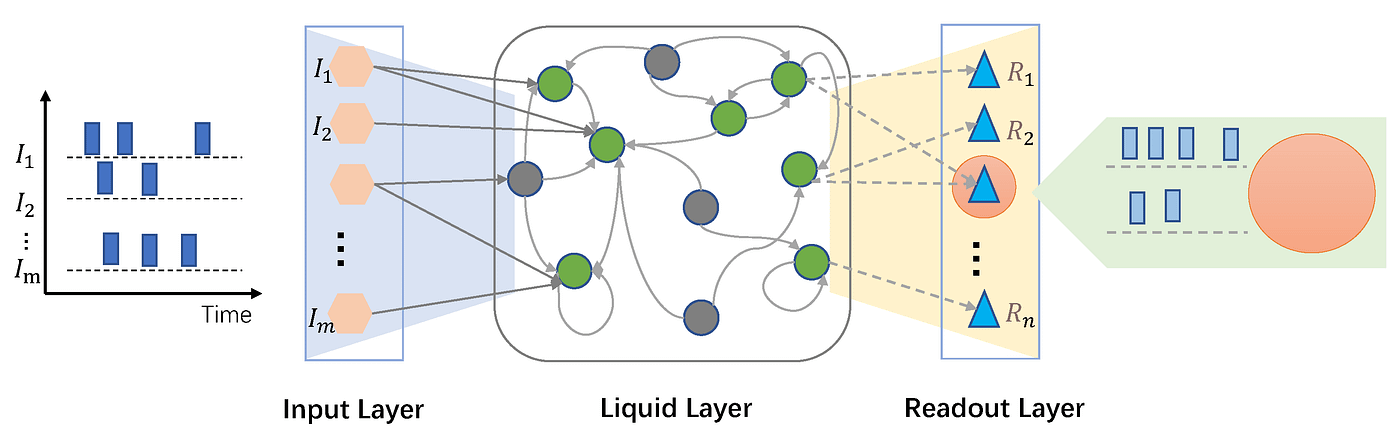
\includegraphics[width=\linewidth]{Image/LNN.png}
    \caption{\centering Diagram of an example LNN model}
    \label{fig:LNN_model}
\end{figure}

\begin{itemize}
    \item \textbf{Input layer:} This layer is required to deal with the reception of the input data \cite{NN_structure}. These data are represented in the form of vectors containing features associated with flights and weather conditions. These features have been carefully and correctly identified during the feature selection process. Moreover, the size of this layer is equivalent to the number of features present within the input data. This initial layer is also utilised to prepare the data to be sent to the liquid layer.
    \item \textbf{Liquid layer:} This layer is the principal component of the LNN model. It is intended to capture any complex temporal relationships that are present within the data \cite{NN_structure}. We defined an ODE function to model such dynamics over time \citep{ODE1,ODE2}. It consists of a network with linear layers and a Tanh activation function in order to introduce non-linearity into the model. Moreover, a solver, namely ‘dopri5’, is adopted to integrate this ODE function over a specified timespan \cite{solver}. Such integration is important for modelling the continuous-time dynamics of the data \citep{ODE1,ODE2}. As most LNNs typically have a single liquid layer, we have followed this trend by using only one such layer\cite{Liquidlayer}. The size of this layer will be a hyperparameter to be adjusted when optimising this model.
    \item \textbf{Output layer:} This layer is responsible for receiving as input the final hidden states of the liquid layer \cite{NN_structure}. By using this received data, this linear-type layer produces a distribution of probabilities over the three target classes \cite{NN_structure}, namely on-time flight, non-weather delay and weather delay. The class with the highest probability is identified as the predicted class.
\end{itemize}

\subsection{Long Short-Term Memory}

\noindent In this section, we will explain the LSTM model developed using the PyTorch library. This model has been built in order to predict if a flight is on-time, delayed for weather conditions or delayed for non-weather conditions.

\subsubsection{Model architecture}

\noindent There are three main components in the architecture of the LSTM model: the input layer, the LSTM layers and the output layer, as shown in Figure \ref{fig:LSTM_model}.

\begin{figure}[H]
    \centering
    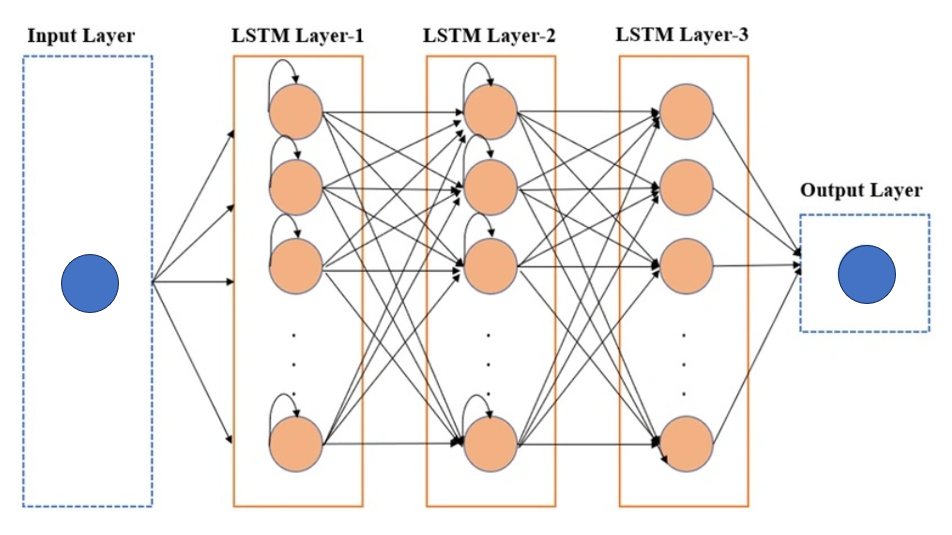
\includegraphics[width=0.9\linewidth]{Image/LSTM.png}
    \caption{\centering Diagram of an example LSTM model}
    \label{fig:LSTM_model}
\end{figure}

\begin{itemize}
    \item \textbf{Input layer:} The input layer is in charge of receiving the input data cite \cite{NN_structure}. These data inputs consist of vectors which represent the features of flight and weather conditions, previously selected during the preprocessing and the feature selection phase. The dimension of these feature vectors is equal to the number of input features. Besides, this layer does not involve any complex transformation. Indeed, it only serves as a starting point for the data sequences introduced into the model.
    \item \textbf{LSTM layers:} These layers can be considered as the principal component of the model. We utilised several stacked LSTM layers during the development of this DL model. As a result, this allows the capture of any complex temporal relationships present in the input data \cite{NN_structure}. In addition, the LSTM layers receive as input the outputs of the previous layer \cite{NN_structure} and generate hidden states initialised at zero for each data sequence. Moreover, the output of the last LSTM layer at the last time step is passed as the input to the output layer. Both the number and the size of these layers are some hyperparameters that will be adjusted when optimising the performance of this model.
    \item \textbf{Output layer:} The output layer is a linear layer which generates a probability distribution over the three classes of the target variable, namely on-time flight, non-weather delay and weather delay \cite{NN_structure}. To generate these class probabilities, this layer uses the hidden states of the last LSTM layer at the last time step and predicts the most likely class based on these probabilities.
\end{itemize}

\subsection{MultiLayer Perceptron}

\noindent In this section, we will present in detail the MLP model that we developed by utilising the PyTorch library. This model is intended for predicting if a flight is on-time, delayed due to weather conditions or delayed due to non-weather conditions.

\subsubsection{Model architecture}

\noindent As we know, the MLP architecture is quite conventional compared with the two previous models. Indeed, the MLP model has three main components in its architecture that can be found in most of NN models: the input layer, the hidden layers and the output layer, as represented in Figure \ref{fig:MLP_model}.

\begin{figure}[H]
    \centering
    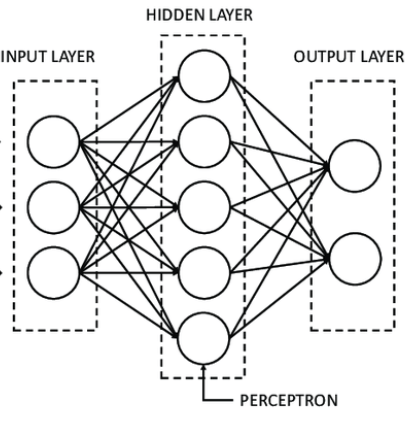
\includegraphics[width=0.6\linewidth]{Image/MLP.png}
    \caption{\centering Diagram of an example MLP model}
    \label{fig:MLP_model}
\end{figure}

\begin{itemize}
    \item \textbf{Input layer:} This layer is responsible for accepting the input data \cite{NN_structure}. These data are in the form of vectors that represent the flight and weather related features determined during feature selection. Moreover, the size of this layer is fixed by the total number of features included in these vectors. This layer does not actually modify the data but passes it on to the hidden layers for further processing. 
    \item \textbf{Hidden layers:} These hidden layers are a series of fully connected layers. These hidden layers follow a particular structure: they consist of a linear layer, a Leaky ReLU activation function and a dropout layer. The Leaky ReLU function is utilised to introduce non-linearity into the model \cite{NN_structure}. In this way, the model is able to capture any complex relationships in the data \cite{NN_structure}. Moreover, the dropout layer is used to reduce the risk of overfitting. Besides, each hidden layer takes as input the outputs of the previous layer \cite{NN_structure}. The number of hidden layers and their sizes are both some hyperparameters that will be adjusted when optimising the performance of the model. 
    \item \textbf{Output layer:} This layer is a classical output layer very similar to those of the other NNs. It is linear and is used to produce a set of probabilities on the three target classes defined when creating the target variable \cite{NN_structure}, explained in section 3.2.3: on-time flight, delays due to non-weather conditions and delays due to weather conditions.
\end{itemize}

\subsection{Loss Function}
\label{Loss_function}

\noindent For the LNN, LSTM and MLP models, we decided to employ the CrossEntropyLoss function. Indeed, this function is very adapted to multiclass classification tasks \cite{crossentropyloss}. This function is set by the following equation \cite{crossentropyloss_equation}:
\begin{align}
\text{CrossEntropyLoss}(y, p) &= -\sum_{c} y_{c} \log(p_{c})
\label{CrossEntropyLoss}
\end{align}

\noindent \text{where \( y_{i} \) is the actual label and \( {p}_{i} \) is the probability predicted by the model for the class \( i \)}

\noindent This loss function from PyTorch is a combination of the application of the softmax function and  the loss computation. In other words, this  function first converts the logits produced by the output layer into class probabilities \cite{crossentropyloss}. Subsequently, it calculates the loss between these probabilities obtained and the actual class labels by using the equation \ref{CrossEntropyLoss}.

\subsection{Optimizer}

\noindent We decided to employ the Adaptive Moment Estimation (Adam) optimizer for training the LNN, LSTM, and MLP models. We opted for this optimizer because it is indispensable for adjusting the weights of DL models \cite{Adam_optimizer1}. Indeed, Adam is well-suited for NNs like LNNs, LSTMs, and MLPs as it combines the benefits of gradient descent methods with momentum and adaptive learning rate adjustment techniques \cite{Adam_optimizer}. One of the principal advantages of this optimizer is its capacity to provide a very fast convergence towards the optimal solution \cite{Adam_optimizer1}. Indeed, this is necessary for the optimisation of model performance in a reasonable time \cite{Adam_optimizer1}. In addition, Adam is acknowledged for its robustness, which is important when dealing with some complex problems, such as flight delay prediction. The Adam optimizer mainly uses the learning rate as a key parameter. This parameter is set during the optimisation process of the hyperparameters of the DL models.

\subsection{Activation function}

\noindent As part of DL model training, activation functions are used to propagate gradients. In this way, they ensure that the models can learn effectively. Moreover, they influence how information is transformed and propagated throughout the network \cite{leaky_relu1}.

\noindent We selected to utilise the Leaky ReLU activation function in the structure of the MLP model. This activation function enables the neural networks to capture all non-linear relationships present in the input data and to process complex phenomena in the data \cite{leaky_relu1}. This function is defined by \cite{leaky_relu_equation}:
\begin{align}
f(x) = 
\begin{cases} 
x & \text{si } x \geq 0 \\
\alpha x & \text{si } x < 0 
\end{cases}
\label{Leaky_ReLU}
\end{align}

\noindent where \(\alpha\) is a positive coefficient which, by default, is defined around 0.01.

\noindent As the equation \ref{Leaky_ReLU} shows, this function introduces a slope for negative input values \cite{leaky_relu}. This activation function has many significant advantages. Indeed, it correctly handles the problem where neurons stop learning if input values are negative or if gradients are set to zero with the introduction of the slope in the equation \cite{leaky_relu}. It also improves overall network learning. Finally, it is simple to implement and helps greatly to improve the robustness of the model.

\noindent Moreover, we also chose to adopt the tanh activation function in the architecture of the LNN model. As with the Leaky ReLU function, the tanh function introduces non-linearity into the NN. This allows the model to learn more complex non-linear relationships between the input and the output data \cite{Tanh3}. This function is defined by \citep{Tanh1,Tanh3}: 
\begin{align}
f(x) = \frac{e^x - e^{-x}}{e^x + e^{-x}}
\label{tanh}
\end{align}

\noindent where x represents the input value and e represents the exponential, a mathematical term.

\noindent As shown in equation 3.4, it transforms the input values to obtain the output values in the range -1 to 1 \citep{Tanh1,Tanh3}. Moreover, the function is symmetrical around the origin, meaning that it generates negative results for negative input values and positive results for positive input values \cite{Tanh3}. This function also enables the models to obtain good performance. The only major limitation of this tanh function is that it can be confronted with the vanishing gradient problem \citep{Tanh1,Tanh3}.

\section{Hyperparameters Optimisation}
\label{hyperparameters_optimisation}

\noindent We chose to perform an optimisation of the hyperparameters, which is an absolutely fundamental step in the development and training of DL models. Indeed, this selection of hyperparameter values is a complex task that can have a major impact on the performance of the LNN, MLP and LSTM models. The aim of this optimisation is to identify the optimum combination of hyperparameters from among those tested in order to obtain models that are as accurate as possible. The table below \ref{tab:hyperparameters} illustrates the hyperparameters tested for each model.

\setlength\LTleft{1cm}
\begin{longtable}{p{4cm} p{9cm}}
\caption{List of Models and Their Hyperparameters} \label{tab:hyperparameters} 
\\\hline
\textbf{Models} & \textbf{Hyperparameters} \\ \hline
\endfirsthead

\hline
\textbf{Models} & \textbf{Hyperparameters} \\ \hline
&\\
\endhead

\hline \multicolumn{2}{r}{{Continued on next page}} \\ \hline
&\\
\endfoot

\hline
\endlastfoot
&\\
LNN & Learning rate, Number of Epochs, Batch size, Number of hidden nodes\\
&\\
LSTM & Learning rate, Number of Epochs, Number of layers, Number of hidden nodes\\ 
&\\
MLP & Learning rate, Number of Epochs, Number of layers, Number of hidden nodes\\ 
&\\
\end{longtable}

\noindent Below is a detailed description of each hyperparameter utilised in this thesis: 

\begin{itemize}
    \item \textbf{Learning rate:} The learning rate is an important hyperparameter when training DL models. It determines the amplitude of the network weights updates during backpropagation \cite{learning_rate}. In this way, choosing the right learning rate value is difficult. Indeed, a learning rate too high can lead to the divergence of the model \cite{learning_rate1}. In contrast, a learning rate too low can considerably slow down the phase of convergence. As a result, the model may get locked into local minima \cite{learning_rate1}.
    \item \textbf{Number of epochs:}  The number of epochs represents the number of complete passes the training data makes through the algorithm. \citep{Epochs_batch,Epochs_batch1} One epoch means that each sample in the training dataset has the opportunity to update the model weights \citep{Epochs_batch,Epochs_batch1}. Therefore, the number of epochs is one of the most important hyperparameters. It has a direct influence on the speed and the quality of training. In this way, it is necessary to optimise it while limiting some excessive adjustments. Indeed, a number of epochs that is too low may cause the model to be undertrained \cite{Epochs_batch1}. This will surely lead to underfitting, and therefore inevitably resulting in poor predictions in terms of performance. On the contrary, a number of epochs too high may lead the model to train without any potential benefit. This will cause the model to overfit \cite{Epochs_batch1}. In addition, it will struggle to obtain overall good performance during the predictions.
    \item \textbf{Batch size:} The batch size is the number of samples utilised before any update is made to the weights of the model during the training \citep{Epochs_batch,Epochs_batch1}. Similar to the number of epochs, the batch size is one of the key hyperparameters. It influences the speed and stability of the learning process. A batch size too small enables more updates to be made to the model weights. In this way, convergence may become more precise \cite{Epochs_batch2}. This can also introduce some noise and instabilities during updates. A batch size too large produces a more stable estimation of the gradient. It also uses more resources in memory and can seriously increase the speed of training \cite{Epochs_batch2}.
    \item \textbf{Number of hidden nodes:} The number of hidden nodes corresponds to the size of the hidden layers of a NN. This hyperparameter is delicate as it may affect the speed and the complexity during the training process. On the one hand, a smaller size can seriously restrict the learning capacities of the model. On the other hand, a particularly large size may help the model capture more complex relationships present in the data \cite{Hyperparameters1}. Nevertheless, it can also raise the risk of overfitting. It may even slow down the training process as well as needing more computing power and more memory \cite{Hyperparameters1}. 
    \item \textbf{Number of layers:} The number of layers represents the layer count between the input and output of the NN. This hyperparameter directly affects the depth and the complexity of the network. In this way, it is necessary to select the right number of layers for optimising the model. Indeed, as a NN contains more layers, the more complex relationships can be learned \cite{Hyperparameters}. It can also help to improve the performance on difficult tasks. Unfortunately, it may in some cases increase the risk of overfitting \cite{Hyperparameters1}. It can even result in gradient problems such as vanishing or exploding \cite{Gradient}.
\end{itemize}

\noindent Concerning the LSTM and MLP models, we decided to apply the grid search algorithm approach to optimise the hyperparameters. Indeed, this method has been particularly adopted in previous research on flight delay prediction. It allows different combinations of hyperparameters to be explored to identify the one that produces the best performance. This approach was necessary because it enabled us to get the optimal configurations for these two models. 

\noindent Conversely, for the LNN model, we had to optimise the hyperparameters manually for many reasons. Indeed, it was not possible to apply grid search for the LNN because of the extremely long execution time required for a single combination. In addition, considerable computing resources were needed to apply this optimisation method. In the end, we tested each combination of hyperparameters one by one to find the optimal one for the LNN model.

\section{Evaluation}
\label{evaluation}

\noindent The evaluation of different models is important in the context of predicting weather-impacted flight delays. In a multiclass classification problem, it is necessary to choose the appropriate performance metrics to ensure that the models developed correctly satisfy the requirements of the problem. For this thesis, the chosen metrics are: the accuracy, precision, recall and F1-score. These metrics were selected for their relevance in the evaluation of classification problems where imbalances between classes can affect the overall performance of the models. Indeed, these performance metrics are quite necessary to fully evaluate a DL model as part of a 3 class classification, notably when performance may vary depending on the class. With these metrics, we will be able to identify classes that are well handled by the model, as well as highlighting problematic classes. They will also help us to understand the nature of the errors encountered for each class.

\noindent The accuracy \cite{Klu} refers to the proportion of correct predictions out of the total number of predictions achieved. Moreover, the precision \cite{Klu} is measured as the proportion of positive predictions that are really correct out of the total number of positive predictions carried out. In addition, the recall \cite{Klu} value represents the ratio of truly correct positive predictions out of the total number of truly positive instances. Finally, the F1-score \cite{Klu} corresponds to the harmonic mean of the precision and the recall, thus delivering a reasonable balance between both of these measures.

\noindent These performance metrics can be computed by using the following equations \cite{Harikri}:
\begin{align}
\text{Accuracy} &= \frac{TN + TP}{TN + FP + TP + FN} \\ 
\text{Precision} &= \frac{TP}{TP + FP}\\
\text{Recall} &= \frac{TP}{TP + FN} \\ 
\text{F1-score} &= 2 \times \frac{\text{Precision} \times \text{Recall}}{\text{Precision} + \text{Recall}}
\end{align}

\noindent where TP is the number of true positives, TN the number of true negatives, FP the number of false positives and FN the number of false negatives.

\noindent We also employed the confusion matrix to evaluate our DL models. Indeed, this matrix is an important tool, especially when dealing with multiclass classification problems. Besides, this matrix is designed to compare the actual and predicted values for each class \cite{Confusion_matrix2}. Through this comparison, the confusion matrix enables us to better visualise and understand the predictions carried out by the models \cite{Confusion_matrix1}.

\noindent As discussed in section \ref{problem_definition}, this problem is a three-class classification. In this way, the confusion matrix employed to evaluate our models takes the form of a 3x3 matrix. Each element of the matrix represents the number of predictions made for each possible combination of actual class and predicted class. An example of the confusion matrix for three classes is shown below:

\begin{figure}[H]
    \centering
    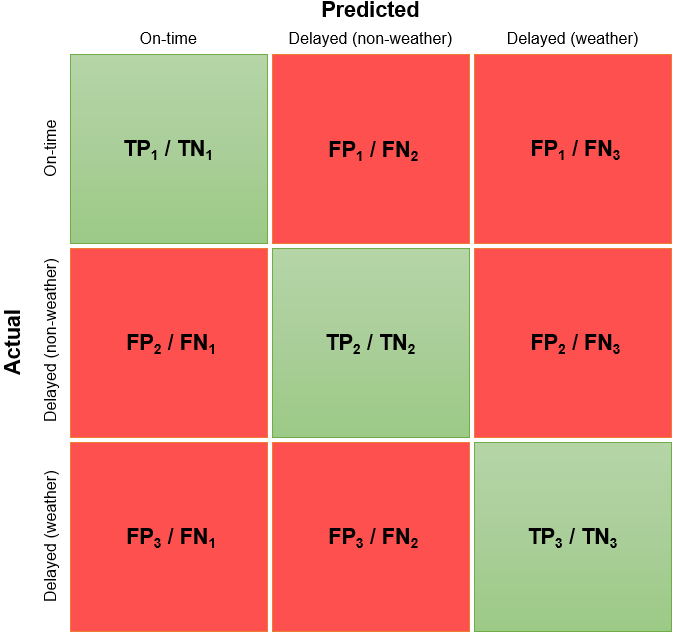
\includegraphics[width=0.75\linewidth]{Image/confusion_matrix_example.png}
    \caption{Structure of a confusion matrix for a three-class classification task}
    \label{fig:confusio,_matrix_example}
\end{figure}

\noindent Using this matrix, we were able to visualise more easily the distribution of correct and incorrect predictions for each class. As a result, we gained a more global view of the performance of the model \cite{Confusion_matrix1}. Indeed, we identified directly the classes for which the model had some difficulties by analysing the matrix \cite{Confusion_matrix2}. Once we identified them, we attempted to adjust the optimisation approaches to improve the accuracy for these classes. Moreover, the confusion matrix provides a better understanding of the imbalances between classes. This is important for the correct interpretation of the previously mentioned performance metrics \citep{Confusion_matrix1,Confusion_matrix2}.

\noindent Moreover, we also tested the overfitting of the models to evaluate them. This test consists of comparing the loss function on the training data with the loss function on the validation data obtained during training \cite{Overfitting}. As mentioned in the section \ref{Loss_function}, we employed the CrossEntropyLoss function. This comparison is necessary to have a precise view of the performance of the models on the training and validation datasets. Indeed, if we notice that the model fits the training data too well, there is a good chance that this might considerably reduce the ability of the model to generalise correctly on unseen data, namely the validation data. Therefore, by monitoring the values of the loss function for both datasets, we will be able to identify and try to attenuate overfitting problems.

\chapter{Results \& Discussions}

%XXX tableau mon meilleur résultat avec les autres tableaux
%XXX comparer ML/DL
%XXX weather_score
%XXX fix the label chapter

\noindent To run all the experiments conducted in this thesis, we used High-Performance Computing (HPC) via the Crescent 2 platform at Cranfield University. This advanced system enabled us to utilise an Nvidia T4 16GB GPU with 8 CPUs. The choice of this GPU was driven by its performance and energy efficiency, making model training faster and more efficient. These two advantages were decisive for carrying out the experiments and obtaining results as soon as possible.

\section{Exploratory Data Analysis}

\noindent In this section, we will analyse in depth the data used for the prediction of flight delays due to weather conditions. For this purpose, we carried out an EDA, which is an important phase in this thesis.Note that the EDA was performed after handling missing values and creating the target variable to work on high-quality and reliable data. This approach allows us to understand key features of the dataset and to identify the relevant patterns \cite{EDA}. It also enables us to detect anomalies in the data \cite{EDA}. In addition, this analysis gives precious insights into the distribution of variables and the relationships between the features \cite{EDA}. It also indicates factors affecting delays. This EDA will serve as a solid basis for the implementation of DL models.

\noindent Firstly, as part of the EDA, we plotted several graphs based on the flight data to help us understand better the dataset and identify any potential trends.

\begin{figure}[H]
    \centering
    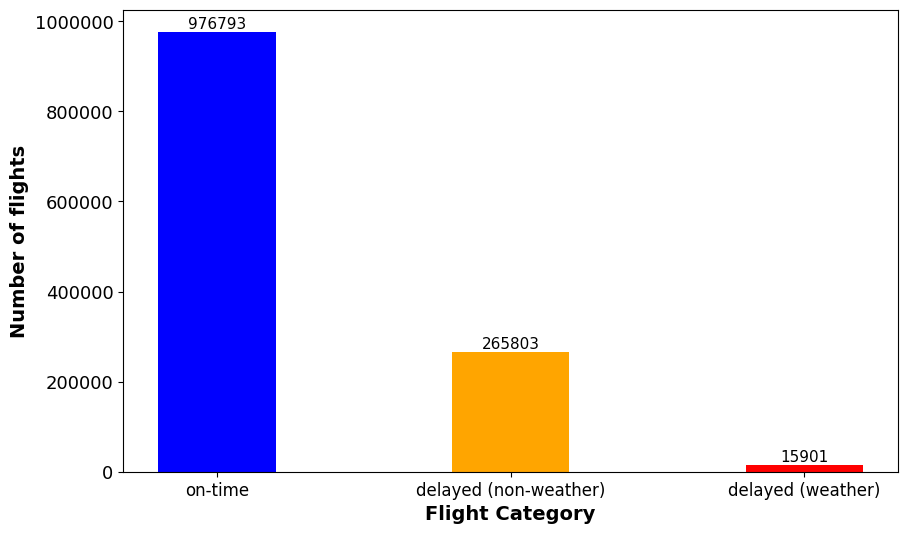
\includegraphics[width=0.85\linewidth]{Image/EDA_1.png}
    \caption{\centering Distribution of flights}
    \label{fig:EDA_1}
\end{figure}

\noindent Figure \ref{fig:EDA_1} shows the distribution of flights. It can be seen that the majority of flights are on time, indicating that most flights arrive without serious delay. This category is by far the most frequent of the three categories. We observe that a considerable number of flights are delayed due to non-weather-related reasons. This category represents a notable proportion of flights, but is much less frequent than on-time flights. Finally, the least frequent category concerns flights delayed due to weather-related reasons. Thus, we note a major imbalance in the flight data in relation to these three categories. This observation coincides with those of other research studies concerning the imbalance in the data used to predict flight delays.

\begin{figure}[H]
    \centering
    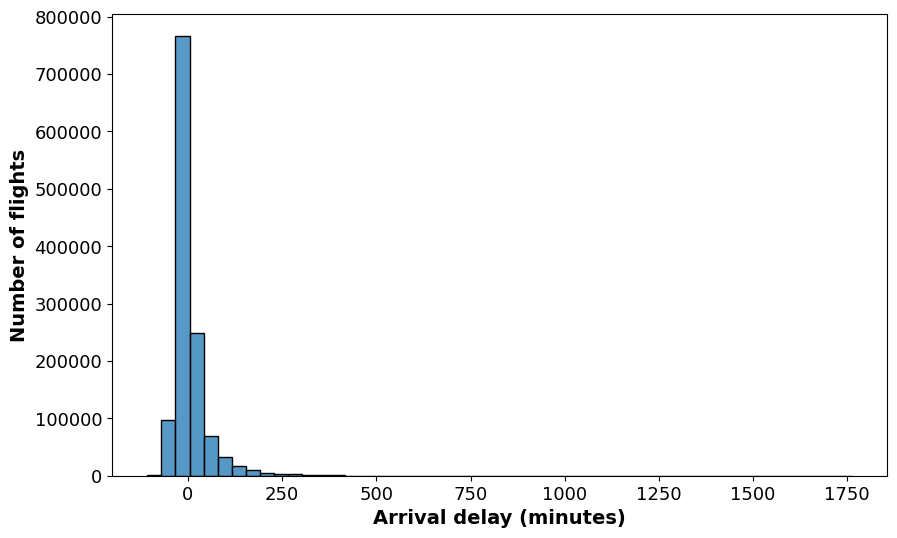
\includegraphics[width=0.85\linewidth]{Image/EDA_2.png}
    \caption{\centering Distribution of arrival flight delays}
    \label{fig:EDA_2}
\end{figure}

\noindent Figure \ref{fig:EDA_2} presents the distribution of arrival delays. As expected, most flights have a small or no delay. This is indicated by the high peak on the left of the graph, near zero minutes delay. We also note that the frequency of flights decreases rapidly as the length of delay increases. However, there is a notable proportion of flights with serious delays. Some of these flights with considerable delays are due to weather conditions. 

\begin{figure}[H]
    \centering
    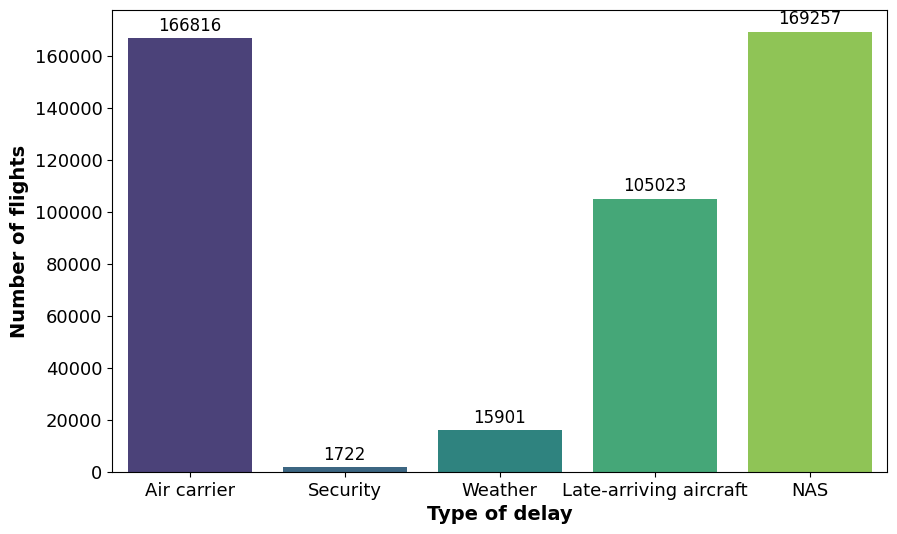
\includegraphics[width=0.85\linewidth]{Image/EDA_3.png}
    \caption{\centering Distribution of causes of delay}
    \label{fig:EDA_3}
\end{figure}

\noindent Figure \ref{fig:EDA_3} shows the distribution of flight delay causes. We can see that weather delays are less frequent than some other causes, such as air carrier and NAS delays. Although lower in frequency, weather delays may be particularly unpredictable. This low proportion necessitates the integration of more precise weather data in order to improve the prediction of weather-impacted flight delays. For this reason, we have used weather data collected from the Weather Underground website to identify patterns of weather delays.

\noindent Secondly, during this EDA, we generated many graphs based on weather data. These visualisations provided valuable insights into weather conditions and their possible impact on flight delays.

\begin{figure}[H]
    \centering
    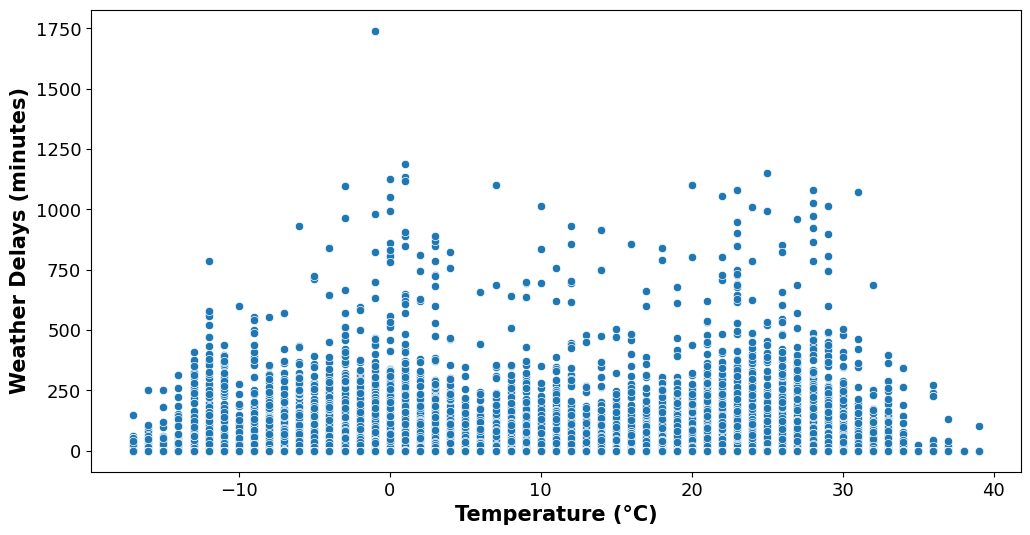
\includegraphics[width=0.87\linewidth]{Image/EDA_4.png}
    \caption{\centering Distribution of weather delays as a function of temperature}
    \label{fig:EDA_4}
\end{figure}

\begin{figure}[H]
    \centering
    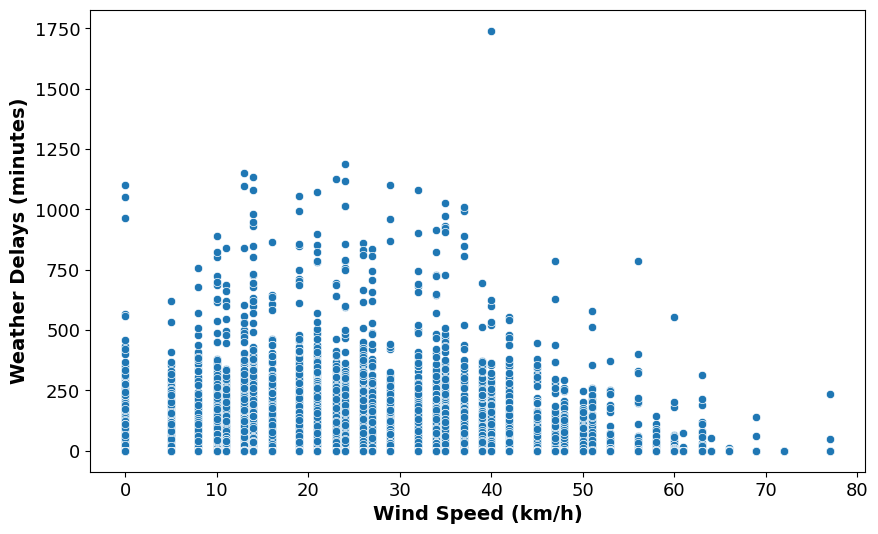
\includegraphics[width=0.87\linewidth]{Image/EDA_5.png}
    \caption{\centering Distribution of weather delays as a function of wind speed}
    \label{fig:EDA_5}
\end{figure}

\noindent Figure \ref{fig:EDA_4} illustrates the dispersion of weather delays  as a function of temperature. There is no obvious linear trend. This indicates that temperature is not highly correlated with weather delays. Furthermore, at very low or very high temperatures, the density of points decreases, indicating a lower frequency of flights in such conditions. However, weather delays in these extreme conditions do not show a considerable increase. All these observations lead us to conclude that weather delays do not depend solely on temperature.

\noindent Figure \ref{fig:EDA_5} shows the dispersion of weather delays  as a function of wind speed. We observe that most of the weather delays are mainly concentrated between 0 and 40 km/h wind speed. Besides, the points representing major weather delays are dispersed across different wind speeds. This indicates that extreme weather delays can happen regardless of wind speed. Although there is no obvious linear trend, there is a slight decrease in the density of long weather delays at very high wind speeds. From all these observations, we can say that even if wind speed contributes to weather delays, it is not the only decisive factor.

\noindent Moreover, during the EDA, we performed an extensive analysis of the weather data to examine in detail its influence on flight delays. In this way, we calculated a weather score for each flight. This score is based on several weather factors, namely temperature, dew point, humidity, wind speed, wind gusts, pressure, precipitation and general weather conditions. This idea was inspired by a previous research carried out by Schultz et al. \cite{Schultz2021} .They calculated the weather score from weather data collected via METAR by using the ATMAP algorithm. We took up the concept of the ATMAP algorithm by classifying the different weather features according to their severity. The classifications for the severity of weather variables were determined through research and arbitrarily. These classifications are then combined to compute an overall score, weighted by the importance of each variable. This score makes it possible to quantify the influence of weather conditions on flight delays in a consistent way. This score is a ratio in the range of 0 to 1. The closer the score is to 1, the more severe the weather conditions.

\begin{figure}[H]
    \centering
    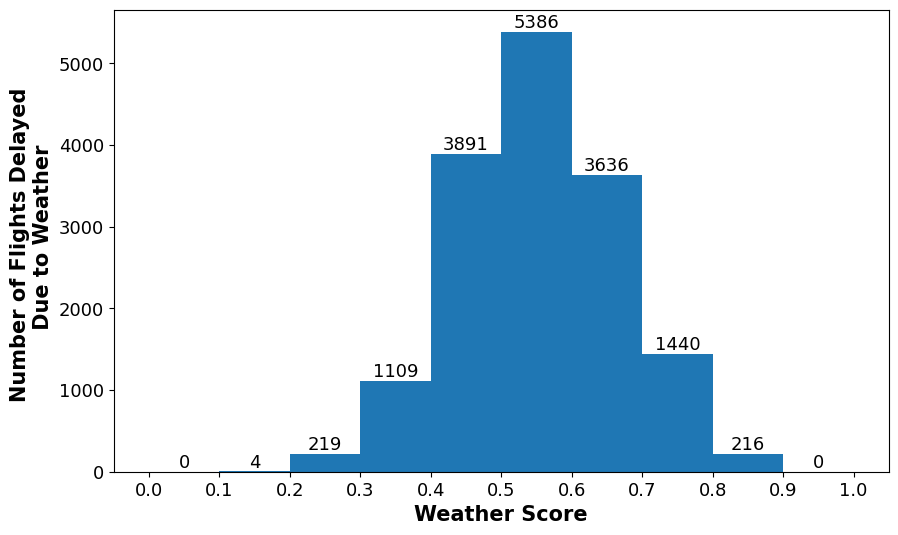
\includegraphics[width=0.9\linewidth]{Image/EDA_6.png}
    \caption{\centering Distribution of flights delayed due to weather conditions by weather score}
    \label{fig:EDA_6}
\end{figure}

\noindent Figure \ref{fig:EDA_6} shows the distribution of flights delayed due to weather conditions by weather score. We observe that most flights delayed due to weather have a weather score between 0.4 and 0.6. This concentration indicates that the moderate weather conditions have a huge impact on weather-related flight delays. On the other hand, we notice that both very low and very high weather scores represent a smaller number of flights delayed due to weather conditions. As a result, we note that extreme weather conditions are not the only cause of flight delays. Moreover, we can say that moderate conditions, when combined, can also cause severe disruption. This observation emphasises the importance of including a full range of weather features in flight delay prediction models. From all these observations, we can affirm that the weather score approach is important and can help to accurately predict weather-impacted flight delays.

\section{Performance and Model Analysis}

\noindent In this section, we will discuss in detail the performance of three DL models, namely the LNN, the LSTM and the MLP. The principal scope of this analysis is to examine the performance of each model in predicting weather-impacted flight delays. For that purpose, we will look at the performance of each model by adopting evaluation methods stated in section \ref{evaluation}. These methods include numerous metrics, namely precision, recall, F1-score, global accuracy and confusion matrix. We will also analyse the loss function curves for each model to understand their behaviour during training and validation.

\noindent The features used to train and evaluate the three models are described in Table \ref{tab:features}. This table shows an extensive list of the features selected, including weather and flight information.

\setlength\LTleft{2cm}
\begin{longtable}{c c p{6cm} }
\caption{List of Features Utilised for Training and Evaluation} \label{tab:features}  \\

\hline
\textbf{S/No} & \textbf{Features} & \textbf{Descriptions}\\ \hline
\endfirsthead

\hline
\textbf{S/No} & \textbf{Features} & \textbf{Descriptions} \\ \hline
\endhead

\hline \multicolumn{3}{r}{{Continued on next page}} \\ \hline
\endfoot

\hline
\endlastfoot
1 & FL\_DATE & The flight date\\ 
2 & CRS\_DEP\_TIME & The scheduled departure time\\ 
3 & DEP\_DELAY & The difference in minutes between the scheduled departure time and the actual departure time\\ 
4 & DEP\_DEL15 & An indicator of whether the flight is delayed on departure\\ 
5 & TAXI\_OUT & The time elapsed between the departure from the boarding gate at the airport of origin and the take-off\\ 
6 & WHEELS\_OFF & The time at which the aircraft's wheels lift off the ground\\ 
7 & CRS\_ARR\_TIME & The scheduled arrival time\\ 
8 & CRS\_ELAPSED\_TIME & The expected duration of the flight in minutes\\ 
9 & Temperature (°C) & The temperature in Celsius\\  
10 & Humidity (\%) & The humidity\\ 
11 & Wind & The wind direction\\ 
12 & Wind Speed (km/h) & The wind speed in km/h\\ 
13 & Pressure (hPa) & The pressure in hPa\\  
14 & Condition & The weather condition\\ 
\end{longtable}

\noindent The 14 features listed in Table \ref{tab:features} were carefully selected for their potential influence on prediction accuracy, in line with the approach explained in section \ref{Feature selection}. Choosing these features is central to guaranteeing that the models can capture some of the underlying dynamics of weather-related flight delays. This approach was based on the analyses presented in Figure \ref{fig:mutual_information} and Table \ref{tab:correlation}.

\begin{figure}[H]
    \centering
    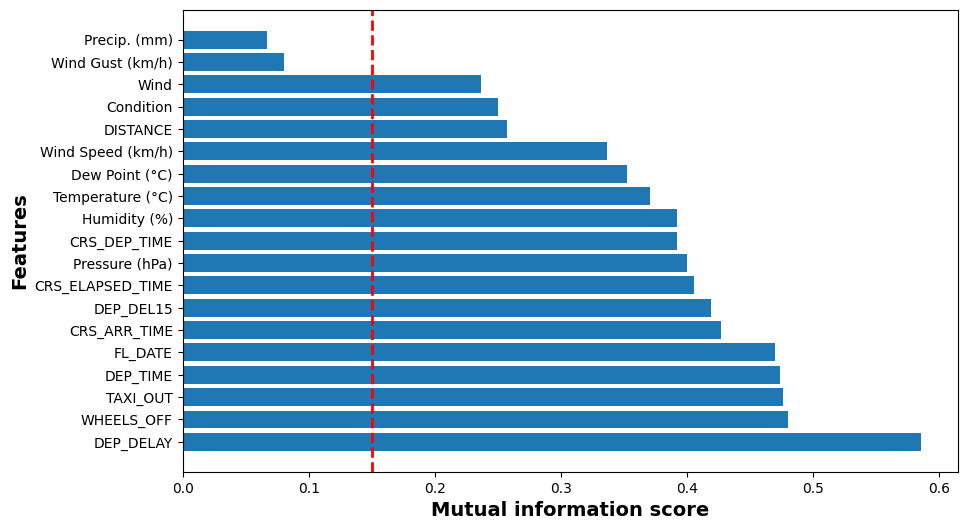
\includegraphics[width=1\linewidth]{Image/mutual_information.png}
    \caption{Mutual information score for features}
    \label{fig:mutual_information}
\end{figure}

\setlength\LTleft{2cm}
\begin{longtable}{c c c}
\caption{Pairs of Features with High Correlation Coefficients} \label{tab:correlation}  \\

\hline
\textbf{Feature 1} & \textbf{Feature 2} & \textbf{Correlation Coefficient}\\ \hline
\endfirsthead

\hline
\textbf{Feature 1} & \textbf{Feature 2} & \textbf{Correlation Coefficient} \\ \hline
\endhead

\hline \multicolumn{3}{r}{{Continued on next page}} \\ \hline
\endfoot

\hline
\endlastfoot
WHEELS\_OFF & DEP\_TIME & 0.832192\\
CRS\_ELAPSED\_TIME & DISTANCE & 0.993380\\
Temperature (°C) & Dew Point (°C) & 0.905055\\
\end{longtable}

\noindent As explained in section \ref{Feature selection}, Figure \ref{fig:mutual_information} allowed us to keep all the features with a score above the threshold of 0.15, marked by the red line. We considered that any features with a score below this threshold had less influence on the prediction model. Subsequently, Table \ref{tab:correlation} enabled us to remove the strong redundancies between pairs of variables with correlation coefficients greater than 0.8. Therefore, in this case, based on Figure \ref{Feature selection} and Table \ref{tab:correlation}, we removed the `DISTANCE', `Dew Point (°C)' and `DEP\_TIME' columns.

\subsection{Liquid Neural Network}

\noindent In this subsection, we will evaluate the performance of the LNN model. As described in section \ref{hyperparameters_optimisation}, we tested many hyperparameter configurations manually due to the consequent execution time. These configurations varied in terms of number of hidden nodes, batch size, learning rate and dropout rate. For each configuration, we performed a series of rigorous tests to evaluate model performance. The results achieved were analysed and compared to measure the impact of each hyperparameter on prediction accuracy. More specifically, we looked at how the number of hidden nodes and the batch size affects model performance. In addition, we studied the effect of using regularisation technique on the model using dropout. We also observed the impact of the learning rate on model convergence. The results of these analyses are discussed below and deliver a detailed evaluation of the performance of each hyperparameter configuration tested. This comparative analysis makes it possible to select the most efficient configurations.

\noindent Given that the LNN model is relatively new, there is no published reference for its hyperparameters. In this way, we had to make some logical and considered decisions when choosing these values. For the learning rate, values of 0.001 and 0.0001 were selected because they are commonly used in ML and DL models \cite{Bengio2012}. For the number of epochs, we tested with 20 and 50 to evaluate the model with a small number and a larger number of iterations. This helps to avoid the risk of overfitting. We did not exceed 50 epochs because the LNN model requires a lot of computational resources. As far as the batch size is concerned, given that the execution time of the model is high, we used fairly large values compared with the usual values \cite{Bengio2012}, testing three options: a small one with 512, a medium one with 1024 and a large one with 2048. For the number of hidden nodes, we followed the same logic. We tested with a small number 50, a medium number 100 and a large number 350. This enables us to find the best compromise between complexity and performance. Finally, to improve the robustness of the model, we used dropout. For configurations employing it, we only used the default value of 0.5.

\noindent \textbf{Configuration 1:}
\begin{multicols}{2}
    \begin{itemize}
        \item Number of hidden nodes = 350
        \item Number of epochs = 20
    \end{itemize}
    \begin{itemize}
         \item Batch size = 1024
         \item Learning rate = 0.0001
    \end{itemize}
\end{multicols}

\setlength\LTleft{1cm}
\begin{longtable}{ c ccc ccc ccc c}
\caption{Performance metrics of the LNN model for configuration 1} \\
\toprule
\textbf{Time} & \multicolumn{3}{c}{\textbf{Class 0}} & \multicolumn{3}{c}{\textbf{Class 1}} & \multicolumn{3}{c}{\textbf{Class 2}} & \textbf{Global} \\
               & Prec. & Rec. & F1  & Prec. & Rec. & F1   & Prec. & Rec. & F1  & Acc. \\
\midrule
\endfirsthead

\caption[]{(continued)} \\
\toprule
\textbf{Time} & \multicolumn{3}{c}{\textbf{Class 0}} & \multicolumn{3}{c}{\textbf{Class 1}} & \multicolumn{3}{c}{\textbf{Class 2}} & \textbf{Global} \\
               & Prec. & Rec. & F1  & Prec. & Rec. & F1   & Prec. & Rec. & F1  & Acc. \\
\midrule
\endhead

\bottomrule
\endfoot

\bottomrule
\endlastfoot

0h             & 0.96  & 0.91 & 0.93 & 0.69  & 0.66 & 0.68  & 0.16  & 0.72 & 0.26 & 85.71\% \\
2h             & 0.96  & 0.91 & 0.93 & 0.68  & 0.60 & 0.64  & 0.13  & 0.77 & 0.23 & 84.56\% \\
4h             & 0.95  & 0.94 & 0.94 & 0.73  & 0.57 & 0.64  & 0.13  & 0.76 & 0.23 & 85.76\% \\
8h             & 0.96  & 0.91 & 0.93 & 0.68  & 0.64 & 0.66  & 0.15  & 0.70 & 0.24 & 85.19\% \\
16h            & 0.96  & 0.92 & 0.94 & 0.68  & 0.64 & 0.66  & 0.15  & 0.67 & 0.24 & 85.48\% \\
24h            & 0.96  & 0.86 & 0.91 & 0.58  & 0.62 & 0.60  & 0.11  & 0.72 & 0.19 & 81.07\% \\
48h            & 0.96  & 0.90 & 0.93 & 0.66  & 0.61 & 0.63  & 0.11  & 0.71 & 0.19 & 83.45\% \\
\end{longtable}

\noindent \textbf{Configuration 2:}
\begin{multicols}{2}
    \begin{itemize}
        \item Number of hidden nodes = 100
        \item Number of epochs = 20
    \end{itemize}
    \begin{itemize}
         \item Batch size = 1024
         \item Learning rate = 0.0001
    \end{itemize}
\end{multicols}

\setlength\LTleft{1cm}
\begin{longtable}{ c ccc ccc ccc c}
\caption{Performance metrics of the LNN model for configuration 2} \\
\toprule
\textbf{Time} & \multicolumn{3}{c}{\textbf{Class 0}} & \multicolumn{3}{c}{\textbf{Class 1}} & \multicolumn{3}{c}{\textbf{Class 2}} & \textbf{Global} \\
               & Prec. & Rec. & F1  & Prec. & Rec. & F1   & Prec. & Rec. & F1  & Acc. \\
\midrule
\endfirsthead

\caption[]{(continued)} \\
\toprule
\textbf{Time} & \multicolumn{3}{c}{\textbf{Class 0}} & \multicolumn{3}{c}{\textbf{Class 1}} & \multicolumn{3}{c}{\textbf{Class 2}} & \textbf{Global} \\
               & Prec. & Rec. & F1  & Prec. & Rec. & F1   & Prec. & Rec. & F1  & Acc. \\
\midrule
\endhead

\bottomrule
\endfoot

\bottomrule
\endlastfoot

0h             & 0.95  & 0.92 & 0.94 & 0.69  & 0.64 & 0.67  & 0.15  & 0.70 & 0.25 & 85.70\% \\
2h             & 0.96  & 0.89 & 0.93 & 0.63  & 0.61 & 0.62  & 0.13  & 0.74 & 0.22 & 83.23\% \\
4h             & 0.95  & 0.93 & 0.94 & 0.70  & 0.64 & 0.67  & 0.15  & 0.67 & 0.25 & 86.16\% \\
8h             & 0.95  & 0.94 & 0.95 & 0.74  & 0.56 & 0.63  & 0.14  & 0.72 & 0.23 & 85.91\% \\
16h            & 0.96  & 0.89 & 0.92 & 0.61  & 0.62 & 0.62  & 0.12  & 0.69 & 0.21 & 82.94\% \\
24h            & 0.96  & 0.89 & 0.93 & 0.62  & 0.61 & 0.62  & 0.12  & 0.70 & 0.21 & 83.24\% \\
48h            & 0.96  & 0.89 & 0.92 & 0.62  & 0.60 & 0.61  & 0.11  & 0.71 & 0.19 & 82.51\% \\
\end{longtable}

\noindent \textbf{Configuration 3:}
\begin{multicols}{2}
    \begin{itemize}
        \item Number of hidden nodes = 350
        \item Number of epochs = 20
    \end{itemize}
    \begin{itemize}
         \item Batch size = 512
         \item Learning rate = 0.0001
    \end{itemize}
\end{multicols}

\setlength\LTleft{1cm}
\begin{longtable}{ c ccc ccc ccc c}
\caption{Performance metrics of the LNN model for configuration 3} \\
\toprule
\textbf{Time} & \multicolumn{3}{c}{\textbf{Class 0}} & \multicolumn{3}{c}{\textbf{Class 1}} & \multicolumn{3}{c}{\textbf{Class 2}} & \textbf{Global} \\
               & Prec. & Rec. & F1  & Prec. & Rec. & F1   & Prec. & Rec. & F1  & Acc. \\
\midrule
\endfirsthead

\caption[]{(continued)} \\
\toprule
\textbf{Time} & \multicolumn{3}{c}{\textbf{Class 0}} & \multicolumn{3}{c}{\textbf{Class 1}} & \multicolumn{3}{c}{\textbf{Class 2}} & \textbf{Global} \\
               & Prec. & Rec. & F1  & Prec. & Rec. & F1   & Prec. & Rec. & F1  & Acc. \\
\midrule
\endhead

\bottomrule
\endfoot

\bottomrule
\endlastfoot

0h             & 0.95  & 0.93 & 0.94 & 0.75  & 0.64 & 0.69  & 0.16  & 0.70 & 0.26 & 86.95\% \\
2h             & 0.96  & 0.90 & 0.93 & 0.67  & 0.61 & 0.64  & 0.13  & 0.76 & 0.22 & 83.85\% \\
4h             & 0.96  & 0.91 & 0.93 & 0.69  & 0.63 & 0.66  & 0.13  & 0.71 & 0.23 & 85.20\% \\
8h             & 0.96  & 0.91 & 0.93 & 0.70  & 0.67 & 0.69  & 0.15  & 0.65 & 0.24 & 85.87\% \\
16h            & 0.96  & 0.90 & 0.93 & 0.67  & 0.67 & 0.67  & 0.15  & 0.67 & 0.24 & 85.16\% \\
24h            & 0.96  & 0.91 & 0.93 & 0.68  & 0.65 & 0.66  & 0.13  & 0.68 & 0.22 & 84.97\% \\
48h            & 0.96  & 0.90 & 0.93 & 0.67  & 0.67 & 0.67  & 0.12  & 0.65 & 0.21 & 84.51\% \\
\end{longtable}

\noindent \textbf{Configuration 4:}
\begin{multicols}{2}
    \begin{itemize}
        \item Number of hidden nodes = 350
        \item Number of epochs = 20
    \end{itemize}
    \begin{itemize}
         \item Batch size = 2048
         \item Learning rate = 0.0001
    \end{itemize}
\end{multicols}

\setlength\LTleft{1cm}
\begin{longtable}{ c ccc ccc ccc c}
\caption{Performance metrics of the LNN model for configuration 4} \\
\toprule
\textbf{Time} & \multicolumn{3}{c}{\textbf{Class 0}} & \multicolumn{3}{c}{\textbf{Class 1}} & \multicolumn{3}{c}{\textbf{Class 2}} & \textbf{Global} \\
               & Prec. & Rec. & F1  & Prec. & Rec. & F1   & Prec. & Rec. & F1  & Acc. \\
\midrule
\endfirsthead

\caption[]{(continued)} \\
\toprule
\textbf{Time} & \multicolumn{3}{c}{\textbf{Class 0}} & \multicolumn{3}{c}{\textbf{Class 1}} & \multicolumn{3}{c}{\textbf{Class 2}} & \textbf{Global} \\
               & Prec. & Rec. & F1  & Prec. & Rec. & F1   & Prec. & Rec. & F1  & Acc. \\
\midrule
\endhead

\bottomrule
\endfoot

\bottomrule
\endlastfoot

0h             & 0.95  & 0.94 & 0.94 & 0.74  & 0.61 & 0.67  & 0.15  & 0.73 & 0.25 & 86.38\% \\
2h             & 0.96  & 0.91 & 0.93 & 0.67  & 0.59 & 0.63  & 0.13  & 0.77 & 0.22 & 84.13\% \\
4h             & 0.95  & 0.93 & 0.94 & 0.71  & 0.58 & 0.63  & 0.13  & 0.74 & 0.23 & 85.30\% \\
8h             & 0.96  & 0.89 & 0.92 & 0.64  & 0.65 & 0.64  & 0.13  & 0.71 & 0.22 & 83.63\% \\
16h            & 0.95  & 0.94 & 0.95 & 0.74  & 0.61 & 0.67  & 0.16  & 0.65 & 0.25 & 86.99\% \\
24h            & 0.95  & 0.93 & 0.94 & 0.71  & 0.61 & 0.66  & 0.14  & 0.66 & 0.23 & 86.07\% \\
48h            & 0.96  & 0.90 & 0.93 & 0.64  & 0.60 & 0.62  & 0.12  & 0.71 & 0.20 & 83.28\% \\
\end{longtable}

\noindent \textbf{Configuration 5:}
\begin{multicols}{2}
    \begin{itemize}
        \item Number of hidden nodes = 100
        \item Number of epochs = 20
    \end{itemize}
    \begin{itemize}
         \item Batch size = 2048
         \item Learning rate = 0.0001
    \end{itemize}
\end{multicols}

\setlength\LTleft{1cm}
\begin{longtable}{ c ccc ccc ccc c}
\caption{Performance metrics of the LNN model for configuration 5} \\
\toprule
\textbf{Time} & \multicolumn{3}{c}{\textbf{Class 0}} & \multicolumn{3}{c}{\textbf{Class 1}} & \multicolumn{3}{c}{\textbf{Class 2}} & \textbf{Global} \\
               & Prec. & Rec. & F1  & Prec. & Rec. & F1   & Prec. & Rec. & F1  & Acc. \\
\midrule
\endfirsthead

\caption[]{(continued)} \\
\toprule
\textbf{Time} & \multicolumn{3}{c}{\textbf{Class 0}} & \multicolumn{3}{c}{\textbf{Class 1}} & \multicolumn{3}{c}{\textbf{Class 2}} & \textbf{Global} \\
               & Prec. & Rec. & F1  & Prec. & Rec. & F1   & Prec. & Rec. & F1  & Acc. \\
\midrule
\endhead

\bottomrule
\endfoot

\bottomrule
\endlastfoot

0h             & 0.96  & 0.87 & 0.91 & 0.59  & 0.63 & 0.61  & 0.12  & 0.72 & 0.21 & 81.60\% \\
2h             & 0.95  & 0.93 & 0.94 & 0.70  & 0.58 & 0.63  & 0.14  & 0.72 & 0.23 & 85.28\% \\
4h             & 0.96  & 0.90 & 0.93 & 0.63  & 0.61 & 0.62  & 0.13  & 0.69 & 0.21 & 83.71\% \\
8h             & 0.95  & 0.94 & 0.94 & 0.73  & 0.58 & 0.64  & 0.14  & 0.69 & 0.23 & 86.04\% \\
16h            & 0.96  & 0.89 & 0.93 & 0.61  & 0.60 & 0.60  & 0.12  & 0.69 & 0.21 & 83.03\% \\
24h            & 0.95  & 0.92 & 0.94 & 0.66  & 0.58 & 0.62  & 0.12  & 0.69 & 0.21 & 84.34\% \\
48h            & 0.96  & 0.90 & 0.93 & 0.62  & 0.60 & 0.61  & 0.12  & 0.69 & 0.20 & 83.11\% \\
\end{longtable}

\noindent \textbf{Configuration 6:}
\begin{multicols}{2}
    \begin{itemize}
        \item Number of hidden nodes = 100
        \item Number of epochs = 20
    \end{itemize}
    \begin{itemize}
         \item Batch size = 512
         \item Learning rate = 0.0001
    \end{itemize}
\end{multicols}

\setlength\LTleft{1cm}
\begin{longtable}{ c ccc ccc ccc c}
\caption{Performance metrics of the LNN model for configuration 6} \\
\toprule
\textbf{Time} & \multicolumn{3}{c}{\textbf{Class 0}} & \multicolumn{3}{c}{\textbf{Class 1}} & \multicolumn{3}{c}{\textbf{Class 2}} & \textbf{Global} \\
               & Prec. & Rec. & F1  & Prec. & Rec. & F1   & Prec. & Rec. & F1  & Acc. \\
\midrule
\endfirsthead

\caption[]{(continued)} \\
\toprule
\textbf{Time} & \multicolumn{3}{c}{\textbf{Class 0}} & \multicolumn{3}{c}{\textbf{Class 1}} & \multicolumn{3}{c}{\textbf{Class 2}} & \textbf{Global} \\
               & Prec. & Rec. & F1  & Prec. & Rec. & F1   & Prec. & Rec. & F1  & Acc. \\
\midrule
\endhead

\bottomrule
\endfoot

\bottomrule
\endlastfoot

0h   & 0.96  & 0.90 & 0.93 & 0.66  & 0.62 & 0.64  & 0.13  & 0.76 & 0.22 & 83.88\% \\
2h   & 0.95  & 0.92 & 0.93 & 0.67  & 0.59 & 0.63  & 0.13  & 0.75 & 0.23 & 84.44\% \\
4h   & 0.95  & 0.94 & 0.94 & 0.73  & 0.57 & 0.64  & 0.13  & 0.73 & 0.23 & 85.69\% \\
8h   & 0.95  & 0.94 & 0.94 & 0.72  & 0.56 & 0.63  & 0.13  & 0.72 & 0.23 & 85.55\% \\
16h  & 0.95  & 0.92 & 0.94 & 0.70  & 0.62 & 0.66  & 0.13  & 0.67 & 0.22 & 85.50\% \\
24h  & 0.95  & 0.94 & 0.95 & 0.74  & 0.57 & 0.64  & 0.14  & 0.68 & 0.23 & 86.22\% \\
48h  & 0.96  & 0.91 & 0.93 & 0.65  & 0.57 & 0.61  & 0.11  & 0.72 & 0.19 & 83.50\% \\
\end{longtable}
\clearpage
\noindent \textbf{Configuration 7:}
\begin{multicols}{2}
    \begin{itemize}
        \item Number of hidden nodes = 50
        \item Number of epochs = 20
    \end{itemize}
    \begin{itemize}
         \item Batch size = 512
         \item Learning rate = 0.0001
    \end{itemize}
\end{multicols}

\setlength\LTleft{1cm}
\begin{longtable}{ c ccc ccc ccc c}
\caption{Performance metrics of the LNN model for configuration 7} \\
\toprule
\textbf{Time} & \multicolumn{3}{c}{\textbf{Class 0}} & \multicolumn{3}{c}{\textbf{Class 1}} & \multicolumn{3}{c}{\textbf{Class 2}} & \textbf{Global} \\
               & Prec. & Rec. & F1  & Prec. & Rec. & F1   & Prec. & Rec. & F1  & Acc. \\
\midrule
\endfirsthead

\caption[]{(continued)} \\
\toprule
\textbf{Time} & \multicolumn{3}{c}{\textbf{Class 0}} & \multicolumn{3}{c}{\textbf{Class 1}} & \multicolumn{3}{c}{\textbf{Class 2}} & \textbf{Global} \\
               & Prec. & Rec. & F1  & Prec. & Rec. & F1   & Prec. & Rec. & F1  & Acc. \\
\midrule
\endhead

\bottomrule
\endfoot

\bottomrule
\endlastfoot

0h   & 0.95  & 0.92 & 0.94 & 0.68  & 0.60 & 0.64  & 0.14  & 0.73 & 0.23 & 84.88\% \\
2h   & 0.96  & 0.88 & 0.92 & 0.61  & 0.64 & 0.62  & 0.14  & 0.72 & 0.23 & 82.79\% \\
4h   & 0.95  & 0.94 & 0.94 & 0.72  & 0.59 & 0.65  & 0.14  & 0.69 & 0.23 & 85.97\% \\
8h   & 0.95  & 0.93 & 0.94 & 0.70  & 0.62 & 0.66  & 0.15  & 0.67 & 0.25 & 85.96\% \\
16h  & 0.96  & 0.89 & 0.92 & 0.60  & 0.61 & 0.60  & 0.13  & 0.70 & 0.21 & 82.61\% \\
24h  & 0.96  & 0.88 & 0.92 & 0.59  & 0.61 & 0.60  & 0.12  & 0.70 & 0.20 & 81.89\% \\
48h  & 0.95  & 0.92 & 0.94 & 0.67  & 0.58 & 0.62  & 0.12  & 0.69 & 0.21 & 84.54\% \\
\end{longtable}

\noindent \textbf{Configuration 8:}
\begin{multicols}{2}
    \begin{itemize}
        \item Number of hidden nodes = 50
        \item Number of epochs = 20
    \end{itemize}
    \begin{itemize}
         \item Batch size = 1024
         \item Learning rate = 0.0001
    \end{itemize}
\end{multicols}

\setlength\LTleft{1cm}
\begin{longtable}{ c ccc ccc ccc c}
\caption{Performance metrics of the LNN model for configuration 8} \\
\toprule
\textbf{Time} & \multicolumn{3}{c}{\textbf{Class 0}} & \multicolumn{3}{c}{\textbf{Class 1}} & \multicolumn{3}{c}{\textbf{Class 2}} & \textbf{Global} \\
               & Prec. & Rec. & F1  & Prec. & Rec. & F1   & Prec. & Rec. & F1  & Acc. \\
\midrule
\endfirsthead

\caption[]{(continued)} \\
\toprule
\textbf{Time} & \multicolumn{3}{c}{\textbf{Class 0}} & \multicolumn{3}{c}{\textbf{Class 1}} & \multicolumn{3}{c}{\textbf{Class 2}} & \textbf{Global} \\
               & Prec. & Rec. & F1  & Prec. & Rec. & F1   & Prec. & Rec. & F1  & Acc. \\
\midrule
\endhead

\bottomrule
\endfoot

\bottomrule
\endlastfoot

0h   & 0.95  & 0.91 & 0.93 & 0.66  & 0.61 & 0.63  & 0.14  & 0.72 & 0.24 & 84.50\% \\
2h   & 0.96  & 0.91 & 0.93 & 0.67  & 0.61 & 0.64  & 0.13  & 0.69 & 0.23 & 84.77\% \\
4h   & 0.96  & 0.90 & 0.93 & 0.63  & 0.61 & 0.62  & 0.14  & 0.71 & 0.23 & 83.66\% \\
8h   & 0.95  & 0.93 & 0.94 & 0.68  & 0.55 & 0.61  & 0.12  & 0.69 & 0.21 & 84.72\% \\
16h  & 0.96  & 0.90 & 0.93 & 0.61  & 0.58 & 0.60  & 0.12  & 0.69 & 0.21 & 83.07\% \\
24h  & 0.96  & 0.90 & 0.93 & 0.62  & 0.59 & 0.60  & 0.12  & 0.67 & 0.21 & 83.27\% \\
48h  & 0.96  & 0.90 & 0.93 & 0.62  & 0.59 & 0.60  & 0.12  & 0.67 & 0.21 & 83.27\% \\
\end{longtable}

\noindent \textbf{Configuration 9:}
\begin{multicols}{2}
    \begin{itemize}
        \item Number of hidden nodes = 50
        \item Number of epochs = 20
    \end{itemize}
    \begin{itemize}
         \item Batch size = 2048
         \item Learning rate = 0.0001
    \end{itemize}
\end{multicols}

\setlength\LTleft{1cm}
\begin{longtable}{ c ccc ccc ccc c}
\caption{Performance metrics of the LNN model for configuration 9} \\
\toprule
\textbf{Time} & \multicolumn{3}{c}{\textbf{Class 0}} & \multicolumn{3}{c}{\textbf{Class 1}} & \multicolumn{3}{c}{\textbf{Class 2}} & \textbf{Global} \\
               & Prec. & Rec. & F1  & Prec. & Rec. & F1   & Prec. & Rec. & F1  & Acc. \\
\midrule
\endfirsthead

\caption[]{(continued)} \\
\toprule
\textbf{Time} & \multicolumn{3}{c}{\textbf{Class 0}} & \multicolumn{3}{c}{\textbf{Class 1}} & \multicolumn{3}{c}{\textbf{Class 2}} & \textbf{Global} \\
               & Prec. & Rec. & F1  & Prec. & Rec. & F1   & Prec. & Rec. & F1  & Acc. \\
\midrule
\endhead

\bottomrule
\endfoot

\bottomrule
\endlastfoot

0h   & 0.95  & 0.93 & 0.94 & 0.70  & 0.58 & 0.63  & 0.13  & 0.68 & 0.22 & 85.28\% \\
2h   & 0.96  & 0.90 & 0.93 & 0.64  & 0.62 & 0.63  & 0.14  & 0.71 & 0.23 & 84.02\% \\
4h   & 0.96  & 0.91 & 0.93 & 0.63  & 0.60 & 0.61  & 0.13  & 0.67 & 0.22 & 83.99\% \\
8h   & 0.96  & 0.90 & 0.93 & 0.62  & 0.59 & 0.61  & 0.13  & 0.67 & 0.22 & 83.44\% \\
16h  & 0.96  & 0.91 & 0.93 & 0.63  & 0.57 & 0.60  & 0.12  & 0.67 & 0.21 & 83.63\% \\
24h  & 0.95  & 0.92 & 0.93 & 0.65  & 0.57 & 0.61  & 0.12  & 0.67 & 0.21 & 84.02\% \\
48h  & 0.95  & 0.92 & 0.94 & 0.66  & 0.56 & 0.60  & 0.12  & 0.67 & 0.20 & 84.31\% \\
\end{longtable}


\noindent \textbf{Configuration 10:}
\begin{multicols}{2}
    \begin{itemize}
        \item Number of hidden nodes = 350
        \item Number of epochs = 50
    \end{itemize}
    \begin{itemize}
         \item Batch size = 2048
         \item Learning rate = 0.0001
    \end{itemize}
\end{multicols}

\setlength\LTleft{1cm}
\begin{longtable}{ c ccc ccc ccc c}
\caption{Performance metrics of the LNN model for configuration 10} \\
\toprule
\textbf{Time} & \multicolumn{3}{c}{\textbf{Class 0}} & \multicolumn{3}{c}{\textbf{Class 1}} & \multicolumn{3}{c}{\textbf{Class 2}} & \textbf{Global} \\
               & Prec. & Rec. & F1  & Prec. & Rec. & F1   & Prec. & Rec. & F1  & Acc. \\
\midrule
\endfirsthead

\caption[]{(continued)} \\
\toprule
\textbf{Time} & \multicolumn{3}{c}{\textbf{Class 0}} & \multicolumn{3}{c}{\textbf{Class 1}} & \multicolumn{3}{c}{\textbf{Class 2}} & \textbf{Global} \\
               & Prec. & Rec. & F1  & Prec. & Rec. & F1   & Prec. & Rec. & F1  & Acc. \\
\midrule
\endhead

\bottomrule
\endfoot

\bottomrule
\endlastfoot

0h   & 0.96  & 0.89 & 0.93 & 0.66  & 0.69 & 0.67  & 0.16  & 0.70 & 0.26 & 84.81\% \\
2h   & 0.95  & 0.93 & 0.94 & 0.72  & 0.62 & 0.67  & 0.15  & 0.73 & 0.25 & 86.21\% \\
4h   & 0.95  & 0.91 & 0.93 & 0.69  & 0.66 & 0.67  & 0.15  & 0.68 & 0.24 & 85.64\% \\
8h   & 0.95  & 0.93 & 0.94 & 0.72  & 0.61 & 0.66  & 0.14  & 0.72 & 0.23 & 85.71\% \\
16h  & 0.97  & 0.86 & 0.91 & 0.58  & 0.62 & 0.60  & 0.11  & 0.75 & 0.20 & 81.07\% \\
24h  & 0.95  & 0.93 & 0.94 & 0.70  & 0.57 & 0.63  & 0.12  & 0.72 & 0.21 & 84.84\% \\
48h  & 0.95  & 0.93 & 0.94 & 0.72  & 0.62 & 0.67  & 0.14  & 0.66 & 0.23 & 86.36\% \\
\end{longtable}

\noindent \textbf{Configuration 11:}
\begin{multicols}{2}
    \begin{itemize}
        \item Number of hidden nodes = 350
        \item Number of epochs = 50
    \end{itemize}
    \begin{itemize}
         \item Batch size = 1024
         \item Learning rate = 0.0001
    \end{itemize}
\end{multicols}

\setlength\LTleft{1cm}
\begin{longtable}{ c ccc ccc ccc c}
\caption{Performance metrics of the LNN model for configuration 11} \\
\toprule
\textbf{Time} & \multicolumn{3}{c}{\textbf{Class 0}} & \multicolumn{3}{c}{\textbf{Class 1}} & \multicolumn{3}{c}{\textbf{Class 2}} & \textbf{Global} \\
               & Prec. & Rec. & F1  & Prec. & Rec. & F1   & Prec. & Rec. & F1  & Acc. \\
\midrule
\endfirsthead

\caption[]{(continued)} \\
\toprule
\textbf{Time} & \multicolumn{3}{c}{\textbf{Class 0}} & \multicolumn{3}{c}{\textbf{Class 1}} & \multicolumn{3}{c}{\textbf{Class 2}} & \textbf{Global} \\
               & Prec. & Rec. & F1  & Prec. & Rec. & F1   & Prec. & Rec. & F1  & Acc. \\
\midrule
\endhead

\bottomrule
\endfoot

\bottomrule
\endlastfoot

0h   & 0.96  & 0.90 & 0.93 & 0.66  & 0.71 & 0.68  & 0.17  & 0.68 & 0.27 & 85.41\% \\
2h   & 0.95  & 0.93 & 0.94 & 0.73  & 0.68 & 0.70  & 0.17  & 0.66 & 0.27 & 87.16\% \\
4h   & 0.96  & 0.91 & 0.93 & 0.69  & 0.67 & 0.68  & 0.15  & 0.66 & 0.24 & 85.61\% \\
8h   & 0.95  & 0.94 & 0.94 & 0.76  & 0.66 & 0.71  & 0.18  & 0.64 & 0.28 & 87.84\% \\
16h  & 0.96  & 0.88 & 0.92 & 0.62  & 0.68 & 0.65  & 0.14  & 0.68 & 0.23 & 83.56\% \\
24h  & 0.96  & 0.91 & 0.93 & 0.69  & 0.65 & 0.67  & 0.13  & 0.68 & 0.22 & 85.20\% \\
48h  & 0.95  & 0.93 & 0.94 & 0.72  & 0.66 & 0.69  & 0.14  & 0.60 & 0.23 & 86.64\% \\
\end{longtable}

\noindent \textbf{Configuration 12:}
\begin{multicols}{2}
    \begin{itemize}
        \item Number of hidden nodes = 100
        \item Number of epochs = 20
        \item Batch size = 2048
    \end{itemize}
    \begin{itemize}
         \item Learning rate = 0.0001
         \item Dropout rate  = 0.5
         \item[\hspace{0pt}]
    \end{itemize}
\end{multicols}

\setlength\LTleft{1cm}
\begin{longtable}{ c ccc ccc ccc c}
\caption{Performance metrics of the LNN model for configuration 12} \\
\toprule
\textbf{Time} & \multicolumn{3}{c}{\textbf{Class 0}} & \multicolumn{3}{c}{\textbf{Class 1}} & \multicolumn{3}{c}{\textbf{Class 2}} & \textbf{Global} \\
               & Prec. & Rec. & F1  & Prec. & Rec. & F1   & Prec. & Rec. & F1  & Acc. \\
\midrule
\endfirsthead

\caption[]{(continued)} \\
\toprule
\textbf{Time} & \multicolumn{3}{c}{\textbf{Class 0}} & \multicolumn{3}{c}{\textbf{Class 1}} & \multicolumn{3}{c}{\textbf{Class 2}} & \textbf{Global} \\
               & Prec. & Rec. & F1  & Prec. & Rec. & F1   & Prec. & Rec. & F1  & Acc. \\
\midrule
\endhead

\bottomrule
\endfoot

\bottomrule
\endlastfoot

0h   & 0.96  & 0.91 & 0.93 & 0.67  & 0.61 & 0.64  & 0.14  & 0.74 & 0.23 & 84.66\% \\
2h   & 0.96  & 0.90 & 0.93 & 0.63  & 0.59 & 0.61  & 0.13  & 0.75 & 0.23 & 83.40\% \\
4h   & 0.96  & 0.91 & 0.94 & 0.66  & 0.59 & 0.63  & 0.13  & 0.72 & 0.22 & 84.49\% \\
8h   & 0.95  & 0.92 & 0.94 & 0.68  & 0.59 & 0.63  & 0.14  & 0.71 & 0.23 & 85.13\% \\
16h  & 0.96  & 0.91 & 0.93 & 0.64  & 0.60 & 0.62  & 0.13  & 0.70 & 0.22 & 84.02\% \\
24h  & 0.95  & 0.92 & 0.94 & 0.67  & 0.59 & 0.63  & 0.13  & 0.69 & 0.22 & 84.82\% \\
48h  & 0.96  & 0.91 & 0.93 & 0.67  & 0.60 & 0.63  & 0.12  & 0.69 & 0.21 & 84.49\% \\
\end{longtable}

\noindent \textbf{Configuration 13:}
\begin{multicols}{2}
    \begin{itemize}
        \item Number of hidden nodes = 100
        \item Number of epochs = 20
        \item Batch size = 1024
    \end{itemize}
    \begin{itemize}
         \item Learning rate = 0.0001
         \item Dropout rate  = 0.5
         \item[\hspace{0pt}]
    \end{itemize}
\end{multicols}

\setlength\LTleft{1cm}
\begin{longtable}{ c ccc ccc ccc c}
\caption{Performance metrics of the LNN model for configuration 13} \\
\toprule
\textbf{Time} & \multicolumn{3}{c}{\textbf{Class 0}} & \multicolumn{3}{c}{\textbf{Class 1}} & \multicolumn{3}{c}{\textbf{Class 2}} & \textbf{Global} \\
               & Prec. & Rec. & F1  & Prec. & Rec. & F1   & Prec. & Rec. & F1  & Acc. \\
\midrule
\endfirsthead

\caption[]{(continued)} \\
\toprule
\textbf{Time} & \multicolumn{3}{c}{\textbf{Class 0}} & \multicolumn{3}{c}{\textbf{Class 1}} & \multicolumn{3}{c}{\textbf{Class 2}} & \textbf{Global} \\
               & Prec. & Rec. & F1  & Prec. & Rec. & F1   & Prec. & Rec. & F1  & Acc. \\
\midrule
\endhead

\bottomrule
\endfoot

\bottomrule
\endlastfoot

0h   & 0.95  & 0.92 & 0.94 & 0.69  & 0.61 & 0.65  & 0.14  & 0.73 & 0.24 & 85.30\% \\
2h   & 0.96  & 0.91 & 0.93 & 0.66  & 0.59 & 0.62  & 0.13  & 0.75 & 0.23 & 84.13\% \\
4h   & 0.96  & 0.91 & 0.93 & 0.66  & 0.62 & 0.64  & 0.13  & 0.70 & 0.23 & 84.64\% \\
8h   & 0.96  & 0.92 & 0.94 & 0.67  & 0.59 & 0.63  & 0.14  & 0.72 & 0.23 & 84.74\% \\
16h  & 0.96  & 0.91 & 0.93 & 0.66  & 0.61 & 0.63  & 0.13  & 0.70 & 0.22 & 84.57\% \\
24h  & 0.95  & 0.92 & 0.94 & 0.67  & 0.59 & 0.63  & 0.13  & 0.70 & 0.21 & 84.53\% \\
48h  & 0.96  & 0.90 & 0.93 & 0.65  & 0.61 & 0.63  & 0.12  & 0.70 & 0.21 & 84.02\% \\
\end{longtable}
\clearpage
\noindent \textbf{Configuration 14:}
\begin{multicols}{2}
    \begin{itemize}
        \item Number of hidden nodes = 350
        \item Number of epochs = 20
        \item Batch size = 1024
    \end{itemize}
    \begin{itemize}
         \item Learning rate = 0.0001
         \item Dropout rate  = 0.5
         \item[\hspace{0pt}]
    \end{itemize}
\end{multicols}

\setlength\LTleft{1cm}
\begin{longtable}{ c ccc ccc ccc c}
\caption{Performance metrics of the LNN model for configuration 14} \\
\toprule
\textbf{Time} & \multicolumn{3}{c}{\textbf{Class 0}} & \multicolumn{3}{c}{\textbf{Class 1}} & \multicolumn{3}{c}{\textbf{Class 2}} & \textbf{Global} \\
               & Prec. & Rec. & F1  & Prec. & Rec. & F1   & Prec. & Rec. & F1  & Acc. \\
\midrule
\endfirsthead

\caption[]{(continued)} \\
\toprule
\textbf{Time} & \multicolumn{3}{c}{\textbf{Class 0}} & \multicolumn{3}{c}{\textbf{Class 1}} & \multicolumn{3}{c}{\textbf{Class 2}} & \textbf{Global} \\
               & Prec. & Rec. & F1  & Prec. & Rec. & F1   & Prec. & Rec. & F1  & Acc. \\
\midrule
\endhead

\bottomrule
\endfoot

\bottomrule
\endlastfoot

0h   & 0.96  & 0.91 & 0.93 & 0.69  & 0.66 & 0.67  & 0.15  & 0.73 & 0.26 & 85.52\% \\
2h   & 0.95  & 0.92 & 0.94 & 0.72  & 0.63 & 0.67  & 0.15  & 0.73 & 0.25 & 86.08\% \\
4h   & 0.95  & 0.93 & 0.94 & 0.72  & 0.64 & 0.68  & 0.15  & 0.70 & 0.25 & 86.45\% \\
8h   & 0.96  & 0.92 & 0.94 & 0.69  & 0.66 & 0.67  & 0.16  & 0.70 & 0.25 & 85.81\% \\
16h  & 0.96  & 0.91 & 0.94 & 0.69  & 0.66 & 0.67  & 0.15  & 0.68 & 0.25 & 85.81\% \\
24h  & 0.96  & 0.92 & 0.94 & 0.70  & 0.65 & 0.67  & 0.14  & 0.69 & 0.24 & 85.71\% \\
48h  & 0.95  & 0.93 & 0.94 & 0.73  & 0.63 & 0.68  & 0.13  & 0.68 & 0.22 & 86.17\% \\
\end{longtable}

\noindent \textbf{Configuration 15:}
\begin{multicols}{2}
    \begin{itemize}
        \item Number of hidden nodes = 350
        \item Number of epochs = 20
        \item Batch size = 2048
    \end{itemize}
    \begin{itemize}
         \item Learning rate = 0.0001
         \item Dropout rate  = 0.5
         \item[\hspace{0pt}]
    \end{itemize}
\end{multicols}

\setlength\LTleft{1cm}
\begin{longtable}{ c ccc ccc ccc c}
\caption{Performance metrics of the LNN model for configuration 15} \\
\toprule
\textbf{Time} & \multicolumn{3}{c}{\textbf{Class 0}} & \multicolumn{3}{c}{\textbf{Class 1}} & \multicolumn{3}{c}{\textbf{Class 2}} & \textbf{Global} \\
               & Prec. & Rec. & F1  & Prec. & Rec. & F1   & Prec. & Rec. & F1  & Acc. \\
\midrule
\endfirsthead

\caption[]{(continued)} \\
\toprule
\textbf{Time} & \multicolumn{3}{c}{\textbf{Class 0}} & \multicolumn{3}{c}{\textbf{Class 1}} & \multicolumn{3}{c}{\textbf{Class 2}} & \textbf{Global} \\
               & Prec. & Rec. & F1  & Prec. & Rec. & F1   & Prec. & Rec. & F1  & Acc. \\
\midrule
\endhead

\bottomrule
\endfoot

\bottomrule
\endlastfoot

0h   & 0.96  & 0.90 & 0.93 & 0.67  & 0.64 & 0.65  & 0.14  & 0.75 & 0.24 & 84.44\% \\
2h   & 0.95  & 0.92 & 0.94 & 0.70  & 0.62 & 0.66  & 0.15  & 0.74 & 0.24 & 85.48\% \\
4h   & 0.96  & 0.91 & 0.93 & 0.67  & 0.64 & 0.66  & 0.15  & 0.70 & 0.24 & 85.04\% \\
8h   & 0.95  & 0.92 & 0.94 & 0.71  & 0.63 & 0.67  & 0.15  & 0.71 & 0.25 & 85.89\% \\
16h  & 0.96  & 0.91 & 0.93 & 0.68  & 0.64 & 0.66  & 0.14  & 0.68 & 0.24 & 85.36\% \\
24h  & 0.95  & 0.92 & 0.94 & 0.69  & 0.64 & 0.66  & 0.14  & 0.68 & 0.24 & 85.56\% \\
48h  & 0.96  & 0.91 & 0.93 & 0.67  & 0.63 & 0.65  & 0.13  & 0.68 & 0.22 & 84.66\% \\
\end{longtable}

\noindent \textbf{Configuration 16:}
\begin{multicols}{2}
    \begin{itemize}
        \item Number of hidden nodes = 100
        \item Number of epochs = 20
        \item Batch size = 2048
    \end{itemize}
    \begin{itemize}
         \item Learning rate = 0.001
         \item Dropout rate  = 0.5
         \item[\hspace{0pt}]
    \end{itemize}
\end{multicols}

\setlength\LTleft{1cm}
\begin{longtable}{ c ccc ccc ccc c}
\caption{Performance metrics of the LNN model for configuration 16} \\
\toprule
\textbf{Time} & \multicolumn{3}{c}{\textbf{Class 0}} & \multicolumn{3}{c}{\textbf{Class 1}} & \multicolumn{3}{c}{\textbf{Class 2}} & \textbf{Global} \\
               & Prec. & Rec. & F1  & Prec. & Rec. & F1   & Prec. & Rec. & F1  & Acc. \\
\midrule
\endfirsthead

\caption[]{(continued)} \\
\toprule
\textbf{Time} & \multicolumn{3}{c}{\textbf{Class 0}} & \multicolumn{3}{c}{\textbf{Class 1}} & \multicolumn{3}{c}{\textbf{Class 2}} & \textbf{Global} \\
               & Prec. & Rec. & F1  & Prec. & Rec. & F1   & Prec. & Rec. & F1  & Acc. \\
\midrule
\endhead

\bottomrule
\endfoot

\bottomrule
\endlastfoot

0h   & 0.96  & 0.92 & 0.94 & 0.70  & 0.67 & 0.69  & 0.17  & 0.70 & 0.27 & 86.24\% \\
2h   & 0.96  & 0.90 & 0.93 & 0.65  & 0.59 & 0.62  & 0.13  & 0.78 & 0.22 & 83.71\% \\
4h   & 0.96  & 0.88 & 0.92 & 0.62  & 0.65 & 0.64  & 0.13  & 0.71 & 0.21 & 82.91\% \\
8h   & 0.96  & 0.92 & 0.94 & 0.67  & 0.56 & 0.61  & 0.13  & 0.77 & 0.22 & 84.15\% \\
16h  & 0.96  & 0.90 & 0.93 & 0.65  & 0.62 & 0.63  & 0.12  & 0.72 & 0.20 & 83.49\% \\
24h  & 0.95  & 0.93 & 0.94 & 0.72  & 0.60 & 0.65  & 0.14  & 0.69 & 0.23 & 85.93\% \\
48h  & 0.96  & 0.92 & 0.94 & 0.68  & 0.61 & 0.64  & 0.13  & 0.70 & 0.22 & 84.91\% \\
\end{longtable}

\noindent \textbf{Configuration 17:}
\begin{multicols}{2}
    \begin{itemize}
        \item Number of hidden nodes = 100
        \item Number of epochs = 20
        \item Batch size = 1024
    \end{itemize}
    \begin{itemize}
         \item Learning rate = 0.001
         \item Dropout rate  = 0.5
         \item[\hspace{0pt}]
    \end{itemize}
\end{multicols}

\setlength\LTleft{1cm}
\begin{longtable}{ c ccc ccc ccc c}
\caption{Performance metrics of the LNN model for configuration 17} \\
\toprule
\textbf{Time} & \multicolumn{3}{c}{\textbf{Class 0}} & \multicolumn{3}{c}{\textbf{Class 1}} & \multicolumn{3}{c}{\textbf{Class 2}} & \textbf{Global} \\
               & Prec. & Rec. & F1  & Prec. & Rec. & F1   & Prec. & Rec. & F1  & Acc. \\
\midrule
\endfirsthead

\caption[]{(continued)} \\
\toprule
\textbf{Time} & \multicolumn{3}{c}{\textbf{Class 0}} & \multicolumn{3}{c}{\textbf{Class 1}} & \multicolumn{3}{c}{\textbf{Class 2}} & \textbf{Global} \\
               & Prec. & Rec. & F1  & Prec. & Rec. & F1   & Prec. & Rec. & F1  & Acc. \\
\midrule
\endhead

\bottomrule
\endfoot

\bottomrule
\endlastfoot

0h   & 0.95  & 0.94 & 0.94 & 0.74  & 0.61 & 0.67  & 0.15  & 0.74 & 0.25 & 86.38\% \\
2h   & 0.96  & 0.89 & 0.92 & 0.62  & 0.61 & 0.62  & 0.13  & 0.77 & 0.22 & 82.89\% \\
4h   & 0.96  & 0.90 & 0.93 & 0.67  & 0.62 & 0.65  & 0.12  & 0.74 & 0.21 & 84.04\% \\
8h   & 0.96  & 0.92 & 0.94 & 0.67  & 0.57 & 0.62  & 0.13  & 0.77 & 0.22 & 84.18\% \\
16h  & 0.95  & 0.92 & 0.94 & 0.70  & 0.62 & 0.66  & 0.14  & 0.69 & 0.23 & 85.53\% \\
24h  & 0.96  & 0.90 & 0.93 & 0.62  & 0.57 & 0.60  & 0.12  & 0.75 & 0.20 & 82.77\% \\
48h  & 0.96  & 0.88 & 0.92 & 0.62  & 0.62 & 0.62  & 0.12  & 0.71 & 0.20 & 82.67\% \\
\end{longtable}

\noindent \textbf{Configuration 18:}
\begin{multicols}{2}
    \begin{itemize}
        \item Number of hidden nodes = 350
        \item Number of epochs = 20
        \item Batch size = 1024
    \end{itemize}
    \begin{itemize}
         \item Learning rate = 0.001
         \item Dropout rate  = 0.5
         \item[\hspace{0pt}]
    \end{itemize}
\end{multicols}

\setlength\LTleft{1cm}
\begin{longtable}{ c ccc ccc ccc c}
\caption{Performance metrics of the LNN model for configuration 18} \\
\toprule
\textbf{Time} & \multicolumn{3}{c}{\textbf{Class 0}} & \multicolumn{3}{c}{\textbf{Class 1}} & \multicolumn{3}{c}{\textbf{Class 2}} & \textbf{Global} \\
               & Prec. & Rec. & F1  & Prec. & Rec. & F1   & Prec. & Rec. & F1  & Acc. \\
\midrule
\endfirsthead

\caption[]{(continued)} \\
\toprule
\textbf{Time} & \multicolumn{3}{c}{\textbf{Class 0}} & \multicolumn{3}{c}{\textbf{Class 1}} & \multicolumn{3}{c}{\textbf{Class 2}} & \textbf{Global} \\
               & Prec. & Rec. & F1  & Prec. & Rec. & F1   & Prec. & Rec. & F1  & Acc. \\
\midrule
\endhead

\bottomrule
\endfoot

\bottomrule
\endlastfoot

0h   & 0.95  & 0.92 & 0.94 & 0.72  & 0.63 & 0.67  & 0.15  & 0.75 & 0.25 & 85.91\% \\
2h   & 0.95  & 0.93 & 0.94 & 0.74  & 0.60 & 0.66  & 0.14  & 0.75 & 0.24 & 86.17\% \\
4h   & 0.96  & 0.92 & 0.94 & 0.69  & 0.64 & 0.66  & 0.15  & 0.71 & 0.24 & 85.61\% \\
8h   & 0.96  & 0.91 & 0.93 & 0.68  & 0.63 & 0.65  & 0.13  & 0.73 & 0.23 & 84.45\% \\
16h  & 0.95  & 0.92 & 0.94 & 0.70  & 0.64 & 0.67  & 0.15  & 0.68 & 0.25 & 86.10\% \\
24h  & 0.96  & 0.91 & 0.93 & 0.67  & 0.61 & 0.64  & 0.13  & 0.72 & 0.22 & 84.46\% \\
48h  & 0.96  & 0.91 & 0.93 & 0.69  & 0.62 & 0.65  & 0.12  & 0.69 & 0.21 & 84.88\% \\
\end{longtable}

\noindent \textbf{Configuration 19:}
\begin{multicols}{2}
    \begin{itemize}
        \item Number of hidden nodes = 350
        \item Number of epochs = 20
        \item Batch size = 2048
    \end{itemize}
    \begin{itemize}
         \item Learning rate = 0.001
         \item Dropout rate  = 0.5
         \item[\hspace{0pt}]
    \end{itemize}
\end{multicols}

\setlength\LTleft{1cm}
\begin{longtable}{ c ccc ccc ccc c}
\caption{Performance metrics of the LNN model for configuration 19} \\
\toprule
\textbf{Time} & \multicolumn{3}{c}{\textbf{Class 0}} & \multicolumn{3}{c}{\textbf{Class 1}} & \multicolumn{3}{c}{\textbf{Class 2}} & \textbf{Global} \\
               & Prec. & Rec. & F1  & Prec. & Rec. & F1   & Prec. & Rec. & F1  & Acc. \\
\midrule
\endfirsthead

\caption[]{(continued)} \\
\toprule
\textbf{Time} & \multicolumn{3}{c}{\textbf{Class 0}} & \multicolumn{3}{c}{\textbf{Class 1}} & \multicolumn{3}{c}{\textbf{Class 2}} & \textbf{Global} \\
               & Prec. & Rec. & F1  & Prec. & Rec. & F1   & Prec. & Rec. & F1  & Acc. \\
\midrule
\endhead

\bottomrule
\endfoot

\bottomrule
\endlastfoot

0h   & 0.96  & 0.91 & 0.93 & 0.68  & 0.60 & 0.64  & 0.13  & 0.79 & 0.22 & 84.15\% \\
2h   & 0.95  & 0.93 & 0.94 & 0.73  & 0.62 & 0.67  & 0.15  & 0.73 & 0.25 & 86.18\% \\
4h   & 0.95  & 0.93 & 0.94 & 0.72  & 0.61 & 0.66  & 0.14  & 0.71 & 0.23 & 85.91\% \\
8h   & 0.96  & 0.89 & 0.93 & 0.66  & 0.63 & 0.65  & 0.12  & 0.74 & 0.21 & 83.62\% \\
16h  & 0.96  & 0.92 & 0.94 & 0.70  & 0.62 & 0.66  & 0.13  & 0.72 & 0.22 & 85.27\% \\
24h  & 0.96  & 0.92 & 0.94 & 0.70  & 0.65 & 0.67  & 0.14  & 0.70 & 0.24 & 85.63\% \\
48h  & 0.96  & 0.91 & 0.94 & 0.68  & 0.61 & 0.64  & 0.12  & 0.71 & 0.21 & 84.70\% \\
\end{longtable}

\noindent \textbf{Configuration 20:}
\begin{multicols}{2}
    \begin{itemize}
        \item Number of hidden nodes = 350
        \item Number of epochs = 50
        \item Batch size = 1024
    \end{itemize}
    \begin{itemize}
         \item Learning rate = 0.0001
         \item Dropout rate  = 0.5
         \item[\hspace{0pt}]
    \end{itemize}
\end{multicols}

\setlength\LTleft{1cm}
\begin{longtable}{ c ccc ccc ccc c}
\caption{Performance metrics of the LNN model for configuration 20}
\label{config20_results}
\\
\toprule
\textbf{Time} & \multicolumn{3}{c}{\textbf{Class 0}} & \multicolumn{3}{c}{\textbf{Class 1}} & \multicolumn{3}{c}{\textbf{Class 2}} & \textbf{Global} \\
               & Prec. & Rec. & F1  & Prec. & Rec. & F1   & Prec. & Rec. & F1  & Acc. \\
\midrule
\endfirsthead

\caption[]{(continued)} \\
\toprule
\textbf{Time} & \multicolumn{3}{c}{\textbf{Class 0}} & \multicolumn{3}{c}{\textbf{Class 1}} & \multicolumn{3}{c}{\textbf{Class 2}} & \textbf{Global} \\
               & Prec. & Rec. & F1  & Prec. & Rec. & F1   & Prec. & Rec. & F1  & Acc. \\
\midrule
\endhead

\bottomrule
\endfoot

\bottomrule
\endlastfoot

0h   & 0.96  & 0.92 & 0.94 & 0.71  & 0.70 & 0.71  & 0.18  & 0.67 & 0.29 & 86.82\% \\
2h   & 0.95  & 0.92 & 0.94 & 0.72  & 0.67 & 0.70  & 0.16  & 0.69 & 0.25 & 86.51\% \\
4h   & 0.96  & 0.91 & 0.94 & 0.70  & 0.70 & 0.70  & 0.17  & 0.65 & 0.27 & 86.57\% \\
8h   & 0.96  & 0.92 & 0.94 & 0.70  & 0.67 & 0.68  & 0.16  & 0.69 & 0.26 & 86.16\% \\
16h  & 0.96  & 0.91 & 0.93 & 0.68  & 0.67 & 0.68  & 0.16  & 0.68 & 0.25 & 85.86\% \\
24h  & 0.96  & 0.91 & 0.93 & 0.70  & 0.67 & 0.68  & 0.15  & 0.68 & 0.24 & 85.90\% \\
48h  & 0.96  & 0.92 & 0.94 & 0.71  & 0.67 & 0.69  & 0.14  & 0.65 & 0.23 & 86.08\% \\
\end{longtable}

\noindent The number of hidden nodes is an important hyperparameter that directly affects the prediction capacity of the LNN model. We see that in the tested configurations, values of 50, 100 and 350 hidden nodes were analysed. Configurations with 350 hidden nodes show better overall performance. Regarding class 0, all the configurations display satisfactory performance for this class, although configurations with 350 nodes have slightly superior results compared to other configurations. We note that Configuration 1 with 350 hidden nodes achieves a precision of 0.96 and a recall of 0.91 using weather data collected 2 hours before flight departure. These results are superior to those of Configuration 2 with 100 hidden nodes, which has a precision of 0.96 and a recall of 0.89 for the same timing of weather data collection. Similarly, the performance of Configuration 1 is better than that of Configuration 7 with 50 nodes, which obtains a precision of 0.96 and a recall of 0.88 for the same time interval. Regarding classes 1 and 2, configurations with 350 hidden nodes generally tend to perform slightly better. Given the difficulty of predicting these two classes as well as the influence of other hyperparameters, other configurations may, in some cases, produce slightly better results than those obtained with 350 hidden nodes. We note that Configuration 1 reaches an F1-score of 0.64 for class 1 and 0.23 for class 2, compared to an F1-score of 0.62 for class 1 and 0.22 for class 2 using weather data at a 2-hour interval before flight departure. Thus, in general, we can observe a certain trend in achieving better performance with the use of 350 hidden nodes. This can be explained by the better capacity of the LNN model to capture complex features with a greater number of hidden nodes \cite{Hyperparameters1}. This is crucial for minority classes where the data can be more diverse and less frequent. However, having too many nodes can also lead to overfitting \cite{Hyperparameters1}.

\noindent In addition, batch size is another important hyperparameter affecting the prediction of the LNN model. We tested configurations with batch sizes of 512, 1024 and 2048. We note that configurations with too large a batch size produce less efficient results compared to those with a moderate batch size. While the results for class 0 are excellent regardless of the batch size, there are notable differences in performance for the other two classes with regard to this hyperparameter. For example, Configuration 11 with a batch size of 1024 achieves a precision of 0.96 and a recall of 0.90 for class 0 using weather data collected 0 hours before flight departure. In comparison, Configuration 10 with a batch size of 2048 obtains a precision of 0.96 but a recall of 0.89 for the same period. For classes 1 and 2, Configuration 11 has an F1 score of 0.68 and 0.27 respectively, compared to 0.67 for class 1 and 0.26 for class 2 for Configuration 10. Moreover, we observe that configurations with too small a batch size produce results quite similar to those with a moderate batch size. The only difference is that configurations with too small a batch size show greater instability in terms of performance relative to the timing of weather data collection. Thus, it can be noted that moderate batch sizes are the most suitable choice for the LNN model. This may be due to the fact that larger batch sizes can reduce the frequency of weight updates. As a result, the learning process for classes 1 and 2 may be slowed down. Also, batch sizes that are too small may introduce more variance in the updates \cite{Epochs_batch2}. In this way, it can also have a negative effect on learning.

\noindent Besides, we find that the learning rate is important for the stability of the convergence of the LNN model. We note that configurations with a learning rate of 0.0001 exhibit more stable performance. For instance, configuration 14 with a learning rate of 0.0001 achieves a global accuracy of 86.45\% for weather data collected 0 hours before flight departure. Configuration 18, with a learning rate of 0.001, attains a global accuracy of 85.61\% for the same timing of weather data collection. In some situations, configurations using a learning rate of 0.001 may perform better than those with a learning rate of 0.0001 because of the possible strong influence of other hyperparameters. Moreover, we observe that Configuration 14 with a learning rate of 0.0001 achieves a global accuracy of between 85.52\% and 86.45\%. In comparison, Configuration 16 with a learning rate of 0.001 shows a global accuracy ranging from 82.91\% to 86.24\%. These results demonstrate the stability obtained with configurations having a learning rate of 0.0001. Thus, we can say that a learning rate that is too high can lead to some oscillations and unstable convergence. Using a learning rate of 0.0001 for the model is the most optimised rate for this hyperparameter in order to have good performance. This rate allows the LNN model to converge in a stable manner while avoiding the problem of quick overfitting.

\noindent Moreover, the number of epochs plays an important role in the prediction performance of the LNN model. We note that configurations with 50 epochs produce better performance in terms of F1-score for the two classes 1 and 2. For instance, Configuration 11 with 50 epochs delivers an F1-score of 0.70 for class 1 and 0.27 for class 2 for weather data collected 2 hours before flight departure. Configuration 1 with 20 epochs has an F1-score of 0.64 for class 1 and 0.23 for class 2 employing the same interval of weather data collection. In addition, configurations with 50 epochs allow for better global accuracy compared to those with 20 epochs. Indeed, Configuration 11 shows a maximum global accuracy of 87.84\% while Configuration 1 achieves a maximum global accuracy of 85.71\%. More epochs enable the LNN model to better learn the feature patterns of classes 1 and 2. However, it is important to still consider the possible risk of overfitting if the LNN model is too complex. In this way, regularisation techniques such as dropout become crucial to maintaining the generalisation of this model.

\noindent Furthermore, it is noted that the use of dropout techniques leads to quite interesting performances. Indeed, configurations with a dropout rate of 0.5 show effective regularisation and better performance on classes 1 and 2. We observe that Configuration 20 with a dropout rate of 0.5 achieves an F1-score of 0.71 for class 1 and 0.29 for class 2 for weather data collected 0 hours before flight departure. In comparison, Configuration 11, without dropout, obtains an F1-score of 0.68 for class 1 and 0.27 for class 2. Additionally, configurations with dropout result in more stable performance. All these observations indicate that dropout helps prevent overfitting and improves the generalisation of the model. By applying dropout, a certain degree of robustness is introduced to the model. Thus, the LNN model is forced to learn more general representations that are less specific to individual samples. This is especially beneficial for classes 1 and 2, where overfitting can be a more major problem.

\noindent Finally, we note that the timing of weather data collection has a huge impact on the performance of the model. We see that configurations demonstrate some fluctuations depending on the timing of weather data collection: 
\begin{itemize}
    \item \textbf{0 hours before departure:} We notice that performance is generally good with very high precision for class 0, but frequently lower F1-scores for class 2. For instance, Configuration 1 shows a precision of 0.96 and a recall of 0.91 for class 0. However, for the same configuration, we observe an F1-score of 0.68 for class 1 and 0.26 for class 2. One possible indication is that weather conditions very close to the departure time capture the most accurate data, thus reducing overall uncertainty.
    \item \textbf{2 to 8 hours before departure:} We find that the results in terms of performance fluctuate slightly, with a small reduction for the two classes 1 and 2. For instance, we can see that configuration 1 at 2 hours has a precision of 0.96 and a recall of 0.91 for class 0. Moreover, we observe a drop in the F1-score for class 1 to 0.64 and for class 2 to 0.23. We can explain this perhaps by a reduction in the accuracy of weather forecasts as the time horizon extends.
    \item \textbf{16 to 48 hours before departure:} We can see that there is a tendency for performance to decline. For instance, Configuration 1 with weather data of 48 hours shows a precision of 0.96 and a recall of 0.90 for the class 0, but lower F1-scores for classes 1 and 2 with 0.63 and 0.19 respectively. All this seems to indicate that long-range weather forecasts are less reliable, thereby introducing more noise into the input data of the model.
\end{itemize}

\noindent Based on this descriptive and critical analysis of the results of the LNN model for 20 different hyperparameter configurations, we identified the best value for each hyperparameter: 

\begin{multicols}{2}
    \begin{itemize}
        \item Number of hidden nodes = 350
        \item Number of epochs = 50
        \item Batch size = 1024
    \end{itemize}
    \begin{itemize}
         \item Learning rate = 0.0001
         \item Dropout rate  = 0.5
         \item[\hspace{0pt}]
    \end{itemize}
\end{multicols}
\noindent These hyperparameter values correspond to Configuration 20. Moreover, as illustrated in Table \ref{config20_results}, we note that performance remains stable for this configuration, regardless of the timing of weather data collection. Finally, we decided to select Configuration 20 using weather data collected 0 hours before flight departure as the final LNN model, as it shows the best performance. Below, we will focus on the final model chosen for the LNN by analysing the loss function for training and validation as well as the confusion matrix.

\begin{figure}[H]
    \centering
    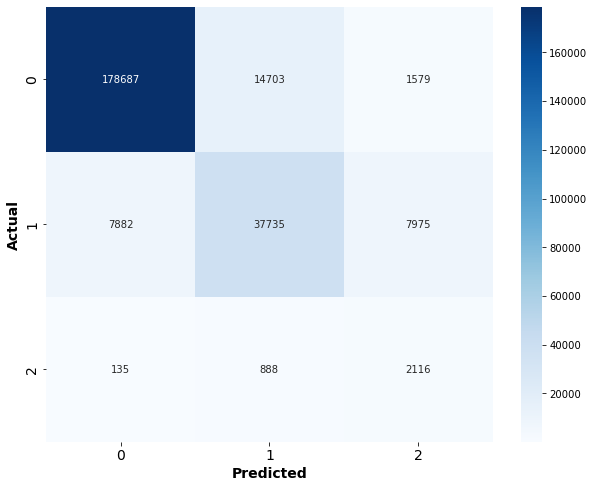
\includegraphics[width=0.73\linewidth]{Image/Confusionmatrix_LNN.png}
    \caption{\centering Confusion matrix for the final LNN model}
    \label{fig:Confusionmatrix_LNN}
\end{figure}

\begin{figure}[H]
    \centering
    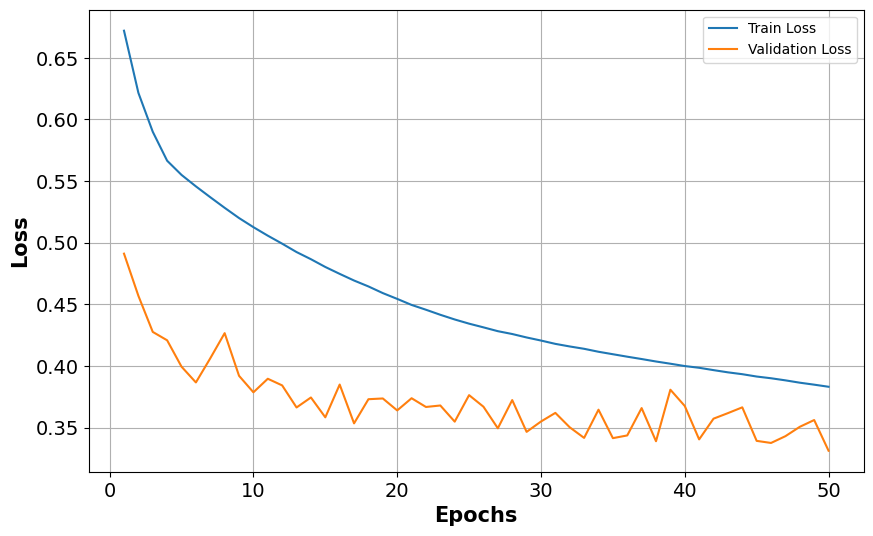
\includegraphics[width=\linewidth]{Image/LNN_loss.png}
    \caption{\centering Training and Validation Loss Over Epochs  for the final LNN model}
    \label{fig:LNN_Loss}
\end{figure}

\noindent Figure \ref{fig:Confusionmatrix_LNN} shows the confusion matrix obtained with the optimal configuration of the LNN model. We can notice that class 0, the majority class within the validation data, is predicted with high accuracy. Indeed, the LNN model achieved a significant number of true positive predictions with 178687 instances, compared to false predictions for the other classes: 14703 for class 1 and 1579 for class 2.  For class 1, we note a huge number of correct predictions with 37735 instances. We can also observe a notable number of false predictions: 7882 predictions as class 0 and 7975 as class 2. This means that, despite the use of SMOTE, the model still has some difficulty in correctly classifying this class from the other two. We can explain this probably by the persistent imbalance in the test data. With regard to class 2, we note that it shows a smaller number of true positive predictions with 2116 instances. This seems logical as class 2 is considered to be the smallest class compared to the others. In addition, class 2 shows a quite high number of false predictions compared to the number of true positive predictions: 135 predictions as class 0 and predictions 888 as class 1. Such results indicate that the LNN model has difficulty in predicting class 2 with a high degree of accuracy. As with class 1, this observation can be attributed to the class imbalance in the test data and the inherent complexity of class 2.

\noindent Figure \ref{fig:LNN_Loss} represents the evolution of the training and validation loss over the number of epochs for the optimal configuration of the LNN model determined previously. We note that the training loss curve demonstrates a continuous decrease. Such observation is an indication that the LNN model is still improving and adjusting its weights optimally across the epochs. This decreasing trend is a sign that the model is learning effectively from the training data. In addition, there is no sign of overfitting on the graph. As for the validation loss curve in orange, it also shows a general tendency to decrease. There are some slight fluctuations in this curve. This may show that the model is experiencing variations within validation data, which can temporarily affect performance. Overall, the decreasing trend in validation loss shows that the LNN model is capable of generalising on unseen data. Besides, the convergence of both curves towards very low and quite similar values proves the capacity of the LNN model to be robust on unseen data.

\subsection{Long Short-Term Memory}

\noindent In this subsection, we will concentrate mainly on evaluating the performance of the LSTM model for predicting weather-impacted flight delays. As described in section \ref{hyperparameters_optimisation}, we utilised a grid search approach. This method enables us to test the following hyperparameters: learning rate, number of epochs, number of layers and number of hidden nodes.  From this exhaustive research, we identified the optimal combinations of these hyperparameters to maximise the accuracy of flight delay predictions. Below is a descriptive and critical analysis of the results obtained with different LSTM configurations. The results also delivered major insights into the ability of the LSTM model to predict weather-related flight delays.

\setlength\LTleft{4cm}
\begin{longtable}{c c}
\caption{Tested hyperparameters in LSTM model} \label{tab:LSTM_hyperparameters} 
\\\hline
\textbf{Hyperparameters} & \textbf{Value} \\ \hline
\endfirsthead

\hline
\textbf{Hyperparameters} & \textbf{Value}  \\ \hline
&\\
\endhead

\hline \multicolumn{2}{r}{{Continued on next page}} \\ \hline
&\\
\endfoot

\hline
\endlastfoot
Learning rate & 0.001, 0.0001\\
Number of Epochs &  20, 50\\ 
Number of layers & 2, 5, 10\\ 
Number of hidden nodes & 50, 100, 150\\
\end{longtable}

\noindent Table \ref{tab:LSTM_hyperparameters} presents the hyperparameters tested in the LSTM model. The values of each hyperparameter are listed to show the different configurations explored when optimising the LSTM model. We chose the values of each hyperparameter during the grid search for several specific reasons. For the learning rate, similar to the LNN model, we used values of 0.001 and 0.0001. The reason for this is that in a previous study using the LSTM model, these two values were selected to train and evaluate the model. Concerning the number of epochs and the number of hidden nodes, we used the same values as those used for the LNN model for these two hyperparameters. We made this choice for fairly similar reasons. We did not go beyond 50 epochs because in this case grid search could require large computational resources. For the number of layers, we wanted to test the LSTM model with a small number of 2, a medium number of 5 and a larger number of 10 layers. We did not adopt the same values used in the previous research by S. Kim and E. Park, which employed 1, 2 and 3 layers. This choice was driven by the desire to explore a wider and more complete range of values. Besides, we used a fixed batch size of 1024 and a fixed dropout rate of 0.5 for all the configurations. The choice of fixing the values for these two hyperparameters was indispensable, because otherwise grid search would require a lot of resources and considerable execution time.

\noindent For each weather data collection interval, we will show below the results of the five best hyperparameter configurations for the LSTM model. These configurations were selected based on their performance. By presenting these results, we can compare and analyse the performance of this DL model depending on the time before flight departure of the weather data collection. In this way, we can deliver a general view of the ability of this model to predict with many weather timing scenarios.

\setlength\LTleft{+0.5cm}
\begin{longtable}{>{\centering\arraybackslash}p{2cm} p{12cm}}
\caption{\centering 5 Best hyperparameter configurations for the LSTM model with weather data collected at 0h before flight departure} \label{tab:LSTM_hyperparameters_config_0h} 
\\\hline
\textbf{S/No} & \textbf{Configurations} \\ \hline
\endfirsthead

\hline
\textbf{S/No} & \textbf{Configurations}  \\ \hline
&\\
\endhead

\hline \multicolumn{2}{r}{{Continued on next page}} \\ \hline
\endfoot

\hline
\endlastfoot
\\
1 & batch size=1024, number of epochs=50, number of layers=5, learning 

rate=0.001, dropout rate=0.5, number of hidden nodes=150\\
&\\
2 & batch size=1024, number of epochs=50, number of layers=10, learning 

rate=0.001, dropout rate=0.5, number of hidden nodes=150\\
&\\
3 & batch size=1024, number of epochs=50, number of layers=10, learning 

rate=0.001, dropout rate=0.5, number of hidden nodes=50\\
&\\
4 & batch size=1024, number of epochs=20, number of layers=5, learning 

rate=0.001, dropout rate=0.5, number of hidden nodes=100\\ 
&\\
5 & batch size=1024, number of epochs=50, number of layers=2, learning 

rate=0.0001, dropout rate=0.5, number of hidden nodes=150\\ 
&\\
\end{longtable}

\setlength\LTleft{1cm}
\begin{longtable}{ c ccc ccc ccc c}
\caption{\centering Performance metrics of the LSTM model for the top 5 configurations with weather data collected at 0h before flight departure} \\
\toprule
\textbf{Config.} & \multicolumn{3}{c}{\textbf{Class 0}} & \multicolumn{3}{c}{\textbf{Class 1}} & \multicolumn{3}{c}{\textbf{Class 2}} & \textbf{Global} \\
               & Prec. & Rec. & F1  & Prec. & Rec. & F1   & Prec. & Rec. & F1  & Acc. \\
\midrule
\endfirsthead

\caption[]{(continued)} \\
\toprule
\textbf{Config.} & \multicolumn{3}{c}{\textbf{Class 0}} & \multicolumn{3}{c}{\textbf{Class 1}} & \multicolumn{3}{c}{\textbf{Class 2}} & \textbf{Global} \\
               & Prec. & Rec. & F1  & Prec. & Rec. & F1   & Prec. & Rec. & F1  & Acc. \\
\midrule
\endhead

\bottomrule
\endfoot

\bottomrule
\endlastfoot

1 & 0.96 & 0.92 & 0.94 & 0.71 & 0.66 & 0.68 & 0.16 & 0.74 & 0.26 & 86.14\% \\
2 & 0.95 & 0.93 & 0.94 & 0.73 & 0.62 & 0.67 & 0.16 & 0.74 & 0.26 & 86.48\% \\
3 & 0.94 & 0.94 & 0.94 & 0.73 & 0.60 & 0.66 & 0.16 & 0.71 & 0.26 & 86.47\% \\
4 & 0.95 & 0.94 & 0.94 & 0.73 & 0.60 & 0.66 & 0.15 & 0.75 & 0.25 & 86.24\% \\
5 & 0.95 & 0.93 & 0.94 & 0.71 & 0.62 & 0.66 & 0.15 & 0.72 & 0.25 & 85.81\% \\
\end{longtable}

\setlength\LTleft{+0.5cm}
\begin{longtable}{>{\centering\arraybackslash}p{2cm} p{12cm}}
\caption{\centering 5 Best hyperparameter configurations for the LSTM model with weather data collected at 2h before flight departure} \label{tab:LSTM_hyperparameters_config_2h} 
\\\hline
\textbf{S/No} & \textbf{Configurations} \\ \hline
\endfirsthead

\hline
\textbf{S/No} & \textbf{Configurations}  \\ \hline
&\\
\endhead

\hline \multicolumn{2}{r}{{Continued on next page}} \\ \hline
\endfoot

\hline
\endlastfoot
\\
1 & batch size=1024, number of epochs=50, number of layers=5, learning 

rate=0.001, dropout rate=0.5, number of hidden nodes=50\\
&\\
2 & batch size=1024, number of epochs=50, number of layers=10, learning 

rate=0.001, dropout rate=0.5, number of hidden nodes=150\\ 
&\\
3 & batch size=1024, number of epochs=50, number of layers=5, learning 

rate=0.001, dropout rate=0.5, number of hidden nodes=150\\
&\\
4 & batch size=1024, number of epochs=20, number of layers=10, learning 

rate=0.001, dropout rate=0.5, number of hidden nodes=100\\
&\\
5 & batch size=1024, number of epochs=20, number of layers=2, learning 

rate=0.001, dropout rate=0.5, number of hidden nodes=150\\ 
&\\
\end{longtable}

\setlength\LTleft{1cm}
\begin{longtable}{ c ccc ccc ccc c}
\caption{\centering Performance metrics of the LSTM model for the top 5 configurations with weather data collected at 2h before flight departure} \\
\toprule
\textbf{Config.} & \multicolumn{3}{c}{\textbf{Class 0}} & \multicolumn{3}{c}{\textbf{Class 1}} & \multicolumn{3}{c}{\textbf{Class 2}} & \textbf{Global} \\
               & Prec. & Rec. & F1  & Prec. & Rec. & F1   & Prec. & Rec. & F1  & Acc. \\
\midrule
\endfirsthead

\caption[]{(continued)} \\
\toprule
\textbf{Config.} & \multicolumn{3}{c}{\textbf{Class 0}} & \multicolumn{3}{c}{\textbf{Class 1}} & \multicolumn{3}{c}{\textbf{Class 2}} & \textbf{Global} \\
               & Prec. & Rec. & F1  & Prec. & Rec. & F1   & Prec. & Rec. & F1  & Acc. \\
\midrule
\endhead

\bottomrule
\endfoot

\bottomrule
\endlastfoot

1 & 0.94 & 0.95 & 0.95 & 0.77 & 0.58 & 0.66 & 0.16 & 0.74 & 0.26 & 87.13\% \\
2 & 0.95 & 0.93 & 0.94 & 0.72 & 0.61 & 0.66 & 0.16 & 0.73 & 0.26 & 86.33\% \\
3 & 0.95 & 0.93 & 0.94 & 0.71 & 0.61 & 0.66 & 0.15 & 0.76 & 0.25 & 85.73\% \\
4 & 0.95 & 0.93 & 0.94 & 0.71 & 0.60 & 0.65 & 0.16 & 0.71 & 0.26 & 86.09\% \\
5 & 0.95 & 0.92 & 0.94 & 0.70 & 0.62 & 0.66 & 0.15 & 0.75 & 0.25 & 85.67\% \\
\end{longtable}

\setlength\LTleft{+0.5cm}
\begin{longtable}{>{\centering\arraybackslash}p{2cm} p{12cm}}
\caption{\centering 5 Best hyperparameter configurations for the LSTM model with weather data collected at 4h before flight departure} \label{tab:LSTM_hyperparameters_config_4h} 
\\\hline
\textbf{S/No} & \textbf{Configurations} \\ \hline
\endfirsthead

\hline
\textbf{S/No} & \textbf{Configurations}  \\ \hline
&\\
\endhead

\hline \multicolumn{2}{r}{{Continued on next page}} \\ \hline
\endfoot

\hline
\endlastfoot
&\\
1 & batch size=1024, number of epochs=20, number of layers=5, learning 

rate=0.001, dropout rate=0.5, number of hidden nodes=100\\
&\\
2 & batch size=1024, number of epochs=50, number of layers=2, learning 

rate=0.001, dropout rate=0.5, number of hidden nodes=50\\ 
&\\
3 & batch size=1024, number of epochs=20, number of layers=10, learning 

rate=0.001, dropout rate=0.5, number of hidden nodes=150\\
&\\
4 & batch size=1024, number of epochs=20, number of layers=5, learning 

rate=0.001, dropout rate=0.5, number of hidden nodes=50\\ 
&\\
5 & batch size=1024, number of epochs=20, number of layers=10, learning 

rate=0.0001, dropout rate=0.5, number of hidden nodes=100\\
&\\
\end{longtable}

\setlength\LTleft{1cm}
\begin{longtable}{ c ccc ccc ccc c}
\caption{\centering Performance metrics of the LSTM model for the top 5 configurations with weather data collected at 4h before flight departure} \\
\toprule
\textbf{Config.} & \multicolumn{3}{c}{\textbf{Class 0}} & \multicolumn{3}{c}{\textbf{Class 1}} & \multicolumn{3}{c}{\textbf{Class 2}} & \textbf{Global} \\
               & Prec. & Rec. & F1  & Prec. & Rec. & F1   & Prec. & Rec. & F1  & Acc. \\
\midrule
\endfirsthead

\caption[]{(continued)} \\
\toprule
\textbf{Config.} & \multicolumn{3}{c}{\textbf{Class 0}} & \multicolumn{3}{c}{\textbf{Class 1}} & \multicolumn{3}{c}{\textbf{Class 2}} & \textbf{Global} \\
               & Prec. & Rec. & F1  & Prec. & Rec. & F1   & Prec. & Rec. & F1  & Acc. \\
\midrule
\endhead

\bottomrule
\endfoot

\bottomrule
\endlastfoot

1 & 0.95 & 0.94 & 0.94 & 0.72 & 0.61 & 0.66 & 0.15 & 0.71 & 0.25 & 86.47\% \\
2 & 0.95 & 0.93 & 0.94 & 0.72 & 0.65 & 0.68 & 0.15 & 0.68 & 0.25 & 86.45\% \\
3 & 0.95 & 0.94 & 0.94 & 0.72 & 0.60 & 0.66 & 0.15 & 0.70 & 0.24 & 86.29\% \\
4 & 0.96 & 0.92 & 0.94 & 0.69 & 0.63 & 0.66 & 0.15 & 0.69 & 0.25 & 85.99\% \\
5 & 0.95 & 0.93 & 0.94 & 0.68 & 0.62 & 0.65 & 0.15 & 0.65 & 0.24 & 85.77\% \\
\end{longtable}

\setlength\LTleft{+0.5cm}
\begin{longtable}{>{\centering\arraybackslash}p{2cm} p{12cm}}
\caption{\centering 5 Best hyperparameter configurations for the LSTM model with weather data collected at 8h before flight departure} \label{tab:LSTM_hyperparameters_config_8h} 
\\\hline
\textbf{S/No} & \textbf{Configurations} \\ \hline
\endfirsthead

\hline
\textbf{S/No} & \textbf{Configurations}  \\ \hline
&\\
\endhead

\hline \multicolumn{2}{r}{{Continued on next page}} \\ \hline
\endfoot

\hline
\endlastfoot
\\
1 & batch size=1024, number of epochs=50, number of layers=2, learning 

rate=0.001, dropout rate=0.5, number of hidden nodes=50\\
&\\
2 & batch size=1024, number of epochs=50, number of layers=5, learning 

rate=0.0001, dropout rate=0.5, number of hidden nodes=150\\ 
&\\
3 & batch size=1024, number of epochs=50, number of layers=5, learning 

rate=0.001, dropout rate=0.5, number of hidden nodes=150\\ 
&\\
4 & batch size=1024, number of epochs=50, number of layers=2, learning 

rate=0.001, dropout rate=0.5, number of hidden nodes=150\\
&\\
5 & batch size=1024, number of epochs=20, number of layers=5, learning 

rate=0.001, dropout rate=0.5, number of hidden nodes=100\\
&\\
\end{longtable}

\setlength\LTleft{1cm}
\begin{longtable}{ c ccc ccc ccc c}
\caption{\centering Performance metrics of the LSTM model for the top 5 configurations with weather data collected at 8h before flight departure} \\
\toprule
\textbf{Config.} & \multicolumn{3}{c}{\textbf{Class 0}} & \multicolumn{3}{c}{\textbf{Class 1}} & \multicolumn{3}{c}{\textbf{Class 2}} & \textbf{Global} \\
               & Prec. & Rec. & F1  & Prec. & Rec. & F1   & Prec. & Rec. & F1  & Acc. \\
\midrule
\endfirsthead

\caption[]{(continued)} \\
\toprule
\textbf{Config.} & \multicolumn{3}{c}{\textbf{Class 0}} & \multicolumn{3}{c}{\textbf{Class 1}} & \multicolumn{3}{c}{\textbf{Class 2}} & \textbf{Global} \\
               & Prec. & Rec. & F1  & Prec. & Rec. & F1   & Prec. & Rec. & F1  & Acc. \\
\midrule
\endhead

\bottomrule
\endfoot

\bottomrule
\endlastfoot

1 & 0.95 & 0.93 & 0.94 & 0.71 & 0.65 & 0.68 & 0.16 & 0.67 & 0.26 & 86.45\% \\
2 & 0.95 & 0.94 & 0.94 & 0.74 & 0.60 & 0.66 & 0.15 & 0.68 & 0.25 & 86.60\% \\
3 & 0.95 & 0.93 & 0.94 & 0.73 & 0.62 & 0.67 & 0.14 & 0.73 & 0.24 & 86.07\% \\
4 & 0.95 & 0.93 & 0.94 & 0.73 & 0.61 & 0.66 & 0.15 & 0.72 & 0.24 & 86.21\% \\
5 & 0.96 & 0.93 & 0.94 & 0.71 & 0.60 & 0.65 & 0.14 & 0.72 & 0.24 & 85.77\% \\
\end{longtable}

\setlength\LTleft{+0.5cm}
\begin{longtable}{>{\centering\arraybackslash}p{2cm} p{12cm}}
\caption{\centering 5 Best hyperparameter configurations for the LSTM model with weather data collected at 16h before flight departure} \label{tab:LSTM_hyperparameters_config_16h} 
\\\hline
\textbf{S/No} & \textbf{Configurations} \\ \hline
\endfirsthead

\hline
\textbf{S/No} & \textbf{Configurations}  \\ \hline
&\\
\endhead

\hline \multicolumn{2}{r}{{Continued on next page}} \\ \hline
\endfoot

\hline
\endlastfoot
\\
1 & batch size=1024, number of epochs=20, number of layers=2, learning 

rate=0.001, dropout rate=0.5, number of hidden nodes=150\\
&\\
2 & batch size=1024, number of epochs=20, number of layers=2, learning 

rate=0.001, dropout rate=0.5, number of hidden nodes=100\\ 
&\\
3 & batch size=1024, number of epochs=50, number of layers=10, learning 

rate=0.0001, dropout rate=0.5, number of hidden nodes=100\\ 
&\\
4 & batch size=1024, number of epochs=50, number of layers=2, learning 

rate=0.001, dropout rate=0.5, number of hidden nodes=150\\
&\\
5 & batch size=1024, number of epochs=50, number of layers=5, learning 

rate=0.001, dropout rate=0.5, number of hidden nodes=100\\
&\\
\end{longtable}

\setlength\LTleft{1cm}
\begin{longtable}{ c ccc ccc ccc c}
\caption{\centering Performance metrics of the LSTM model for the top 5 configurations with weather data collected at 16h before flight departure} \\
\toprule
\textbf{Config.} & \multicolumn{3}{c}{\textbf{Class 0}} & \multicolumn{3}{c}{\textbf{Class 1}} & \multicolumn{3}{c}{\textbf{Class 2}} & \textbf{Global} \\
               & Prec. & Rec. & F1  & Prec. & Rec. & F1   & Prec. & Rec. & F1  & Acc. \\
\midrule
\endfirsthead

\caption[]{(continued)} \\
\toprule
\textbf{Config.} & \multicolumn{3}{c}{\textbf{Class 0}} & \multicolumn{3}{c}{\textbf{Class 1}} & \multicolumn{3}{c}{\textbf{Class 2}} & \textbf{Global} \\
               & Prec. & Rec. & F1  & Prec. & Rec. & F1   & Prec. & Rec. & F1  & Acc. \\
\midrule
\endhead

\bottomrule
\endfoot

\bottomrule
\endlastfoot

1 & 0.95 & 0.94 & 0.95 & 0.75 & 0.60 & 0.67 & 0.14 & 0.69 & 0.24 & 86.77\% \\
2 & 0.95 & 0.93 & 0.94 & 0.71 & 0.62 & 0.66 & 0.14 & 0.69 & 0.24 & 86.00\% \\
3 & 0.95 & 0.93 & 0.94 & 0.68 & 0.60 & 0.63 & 0.15 & 0.67 & 0.24 & 85.48\% \\
4 & 0.95 & 0.92 & 0.94 & 0.72 & 0.63 & 0.68 & 0.14 & 0.69 & 0.23 & 86.12\% \\
5 & 0.96 & 0.91 & 0.94 & 0.67 & 0.62 & 0.65 & 0.14 & 0.71 & 0.23 & 85.14\% \\
\end{longtable}

\setlength\LTleft{+0.5cm}
\begin{longtable}{>{\centering\arraybackslash}p{2cm} p{12cm}}
\caption{\centering 5 Best hyperparameter configurations for the LSTM model with weather data collected at 24h before flight departure} \label{tab:LSTM_hyperparameters_config_24h} 
\\\hline
\textbf{S/No} & \textbf{Configurations} \\ \hline
\endfirsthead

\hline
\textbf{S/No} & \textbf{Configurations} \\ \hline
&\\
\endhead

\hline \multicolumn{2}{r}{{Continued on next page}} \\ \hline
\endfoot

\hline
\endlastfoot
\\
1 & batch size=1024, number of epochs=50, number of layers=2, learning 

rate=0.001, dropout rate=0.5, number of hidden nodes=100\\ 
&\\
2 & batch size=1024, number of epochs=50, number of layers=5, learning 

rate=0.001, dropout rate=0.5, number of hidden nodes=100\\
&\\
3 & batch size=1024, number of epochs=20, number of layers=10, learning 

rate=0.001, dropout rate=0.5, number of hidden nodes=100\\
&\\
4 & batch size=1024, number of epochs=50, number of layers=2, learning 

rate=0.0001, dropout rate=0.5, number of hidden nodes=150\\
&\\
5 & batch size=1024, number of epochs=50, number of layers=10, learning 

rate=0.0001, dropout rate=0.5, number of hidden nodes=150\\ 
&\\
\end{longtable}

\setlength\LTleft{1cm}
\begin{longtable}{ c ccc ccc ccc c}
\caption{\centering Performance metrics of the LSTM model for the top 5 configurations with weather data collected at 24h before flight departure} \\
\toprule
\textbf{Config.} & \multicolumn{3}{c}{\textbf{Class 0}} & \multicolumn{3}{c}{\textbf{Class 1}} & \multicolumn{3}{c}{\textbf{Class 2}} & \textbf{Global} \\
               & Prec. & Rec. & F1  & Prec. & Rec. & F1   & Prec. & Rec. & F1  & Acc. \\
\midrule
\endfirsthead

\caption[]{(continued)} \\
\toprule
\textbf{Config.} & \multicolumn{3}{c}{\textbf{Class 0}} & \multicolumn{3}{c}{\textbf{Class 1}} & \multicolumn{3}{c}{\textbf{Class 2}} & \textbf{Global} \\
               & Prec. & Rec. & F1  & Prec. & Rec. & F1   & Prec. & Rec. & F1  & Acc. \\
\midrule
\endhead

\bottomrule
\endfoot

\bottomrule
\endlastfoot

1 & 0.95 & 0.93 & 0.94 & 0.72 & 0.65 & 0.68 & 0.15 & 0.65 & 0.24 & 86.65\% \\
2 & 0.95 & 0.93 & 0.94 & 0.71 & 0.58 & 0.64 & 0.13 & 0.71 & 0.23 & 85.61\% \\
3 & 0.95 & 0.94 & 0.94 & 0.71 & 0.58 & 0.64 & 0.14 & 0.66 & 0.24 & 86.07\% \\
4 & 0.95 & 0.93 & 0.94 & 0.71 & 0.60 & 0.65 & 0.13 & 0.68 & 0.22 & 85.69\% \\
5 & 0.95 & 0.93 & 0.94 & 0.68 & 0.59 & 0.63 & 0.14 & 0.68 & 0.23 & 85.31\% \\
\end{longtable}

\setlength\LTleft{+0.5cm}
\begin{longtable}{>{\centering\arraybackslash}p{2cm} p{12cm}}
\caption{\centering 5 Best hyperparameter configurations for the LSTM model with weather data collected at 48h before flight departure} \label{tab:LSTM_hyperparameters_config_48h} 
\\\hline
\textbf{S/No} & \textbf{Configurations} \\ \hline
\endfirsthead

\hline
\textbf{S/No} & \textbf{Configurations}   \\ \hline
&\\
\endhead

\hline \multicolumn{2}{r}{{Continued on next page}} \\ \hline
\endfoot

\hline
\endlastfoot
\\
1 & batch size=1024, number of epochs=50, number of layers=10, learning 

rate=0.001, dropout rate=0.5, number of hidden nodes=150\\
&\\
2 & batch size=1024, number of epochs=50, number of layers=2, learning 

rate=0.001, dropout rate=0.5, number of hidden nodes=150\\
&\\
3 & batch size=1024, number of epochs=50, number of layers=2, learning 

rate=0.001, dropout rate=0.5, number of hidden nodes=50\\ 
&\\
4 & batch size=1024, number of epochs=20, number of layers=5, learning 

rate=0.001, dropout rate=0.5, number of hidden nodes=150\\ 
&\\
5 & batch size=1024, number of epochs=20, number of layers=5, learning 

rate=0.001, dropout rate=0.5, number of hidden nodes=50\\
&\\
\end{longtable}

\setlength\LTleft{1cm}
\begin{longtable}{ c ccc ccc ccc c}
\caption{\centering Performance metrics of the LSTM model for the top 5 configurations with weather data collected at 48h before flight departure} \\
\toprule
\textbf{Config.} & \multicolumn{3}{c}{\textbf{Class 0}} & \multicolumn{3}{c}{\textbf{Class 1}} & \multicolumn{3}{c}{\textbf{Class 2}} & \textbf{Global} \\
               & Prec. & Rec. & F1  & Prec. & Rec. & F1   & Prec. & Rec. & F1  & Acc. \\
\midrule
\endfirsthead

\caption[]{(continued)} \\
\toprule
\textbf{Config.} & \multicolumn{3}{c}{\textbf{Class 0}} & \multicolumn{3}{c}{\textbf{Class 1}} & \multicolumn{3}{c}{\textbf{Class 2}} & \textbf{Global} \\
               & Prec. & Rec. & F1  & Prec. & Rec. & F1   & Prec. & Rec. & F1  & Acc. \\
\midrule
\endhead

\bottomrule
\endfoot

\bottomrule
\endlastfoot

1 & 0.95 & 0.93 & 0.94 & 0.71 & 0.62 & 0.66 & 0.15 & 0.67 & 0.24 & 86.31\%
\\
2 & 0.96 & 0.92 & 0.94 & 0.70 & 0.66 & 0.68 & 0.14 & 0.66 & 0.23 & 86.02\%
\\
3 & 0.95 & 0.93 & 0.94 & 0.70 & 0.63 & 0.67 & 0.14 & 0.65 & 0.23 & 86.07\%
\\
4 & 0.96 & 0.92 & 0.94 & 0.69 & 0.63 & 0.66 & 0.14 & 0.68 & 0.23 & 85.49\%
\\
5 & 0.95 & 0.94 & 0.94 & 0.73 & 0.58 & 0.64 & 0.13 & 0.69 & 0.22 & 86.06\%
\\

\end{longtable}

\noindent These results show the influence of the learning rate on the performance of this LSTM model. We note that configurations with a learning rate of 0.001 generally perform slightly better than those using 0.0001. Indeed, we observe that almost all configurations in each top 5 adopt a learning rate of 0.001. For example, with weather data collected 0 hours before flight departure, configurations 1 and 2 with a learning rate of 0.001 have global accuracies of 86.14\% and 86.48\% respectively. Configuration 5 with a learning rate of 0.0001 obtains an overall accuracy of 85.81\%. In addition, we find that this trend also appears for other weather data collection timings. Indeed, with weather data collected 24 hours before flight departure, the results demonstrate that configurations having a learning rate of 0.001 achieve a maximum accuracy of 86.65\% compared to 85.69\% for those using a learning rate of 0.0001. We can explain such finding on the basis that a higher learning rate allows the model to converge more quickly towards optimal solutions. However, we need to be careful because this can also increase the risk of exceeding the optimal solutions if the learning rate is too high.

\noindent In addition, the number of epochs has some influence on the prediction performance of the LSTM model. Indeed, we note that configurations with 50 epochs generally perform better. This observation is emphasised by the proportion of configurations with this number of epochs among all the configurations present in the top 5, which is over 60\%. For example, with weather data collected 2 hours before flight departure, configurations 1 and 2 with 50 epochs achieve global accuracies of 87.13\% and 86.33\% respectively. Configuration 5 with 20 epochs obtains an overall accuracy of 85.67\%. Moreover, Configuration 1 shows an F1-score of 0.66 for class 1 and 0.26 for class 2, compared to 0.66 for class 1 and 0.25 for class 2 for Configuration 5. Similar to the learning rate, this trend is present regardless of the timing of weather data collection. For instance, with weather data collected 8 hours before departure, the configuration with 50 epochs obtains a maximum global accuracy of 86.60\% compared to 85.77\% for the configuration with 20 epochs. This confirms that more epochs allow the model to better capture patterns present in the data, thus reducing prediction errors.

\noindent Moreover, we note that the influence of the number of layers on the performance of the model is variable. Indeed, there is no specific number of layers that stands out to generally optimise the performance of the LSTM model. When using weather data collected 0 hours before departure, we observe that configurations with 5 and 10 layers slightly outperform those with only 2 layers. We find that this trend is not consistent for all weather data collection timings. For example, with weather data collected 16 hours before departure, Configuration 1 with 2 layers obtains a global accuracy of 86.77\%, compared to 85.48\% and 85.15\% for Configuration 3 with 10 layers and 5 layers, respectively. Similarly, for weather data collected 24 hours before departure, Configuration 1 with 2 layers shows an F1-score of 0.68 for class 1 and 0.24 for class 2, slightly better than Configuration 2 with 5 layers, which has an F1-score of 0.64 for class 1 and 0.23 for class 2. All these results imply that increasing the number of layers does not systematically improve the performance of this model. This clearly means that increasing the complexity of the LSTM model is not always advantageous for its performance and can even reduce it. In this way, it seems that the effectiveness of the number of layers depends on other factors, especially other hyperparameters and perhaps the timing of weather data collection.

\noindent Besides, we see that the number of hidden nodes in each LSTM layer impacts the ability of the LSTM model to predict accurately. We note that using a higher number of hidden nodes, such as 150, frequently leads to good model performance. Indeed, configurations with this number of hidden nodes are the most represented in the various top 5 configurations compared to those with a lower number of hidden nodes, namely 50 and 100. For instance, when using weather data collected 0 hours before departure, configurations with 150 hidden nodes achieve a maximum global accuracy of 86.48\% compared with 86.24\% for the configuration with 100 hidden nodes. This trend is not uniform across the different weather data collection timings. Indeed, with weather data collected 2 hours before departure, Configuration 1 with 50 nodes displays an F1-score of 0.95 for class 0, 0.66 for class 1 and 0.26 for class 2. In comparison, Configuration 5 with 150 nodes shows relatively lower F1-scores for classes 0 and 2, with 0.94 and 0.25 respectively. In addition, with weather data collected 24 hours before departure, we can see that configurations with 100 nodes have a majority presence in this top 5. Besides, we find that for weather data collected 24 or 48 hours before departure, configurations with 150 nodes are highly present in both top 5. This can mean that the use of weather data collected only a few days before flight departure may require a more complex LSTM model with a larger number of nodes. From all these observations, we can say that the effectiveness of the number of nodes depends strongly on the timing of collection of the weather data and other hyperparameters. Despite the fact that higher numbers of nodes can increase the risk of overfitting, configurations with 150 nodes show slightly better performance and consistency for classes 1 and 2 than those with 100 and 50 hidden nodes.

\noindent Finally, we note that the timing of weather data collection considerably influences the performance of the LSTM model. This influence is not necessarily linear, with important nuances to consider depending on the timing. Moreover, we find a general trend where weather data collected closer to flight departure produces better scores for various performance metrics, albeit with some limitations. For example, with weather data collected 2 hours before departure, configurations achieve a maximum global accuracy of 87.13\%. In comparison, for weather data collected 0 hours before departure, the maximum global accuracy achieved by different configurations is slightly lower at 86.48\%. When we look in detail at the metric performance for each class, we note that the results are slightly better for weather data collected 0 hours before departure rather than 2 hours. For 0 hours, the configurations show a maximum F1-score of 0.68 for class 1 and 0.26 for class 2, compared with 0.66 for class 1 and 0.26 for class 2 for 2 hours. Performance remains relatively stable even for weather data collected well before departure. For example, configurations using weather data collected 24 hours before departure reach a maximum accuracy of 86.65\%. This observation implies that the LSTM model is capable of capturing long-term weather trends that are important for weather delay prediction. There is a slight decrease in performance for weather data collected 48 hours before departure, with a maximum accuracy of 86.31\%. Moreover, we find a decrease in prediction performance for class 2 as the time taken to collect weather data before departure increases. Indeed, the minimum F1-score for class 2 falls from 0.25 with weather data from 0 hours before departure to 0.22 with data collected 48 hours before the flight. This slight decrease appears logical, as it is unlikely that weather data collected 48 hours in advance will remain similar to the weather conditions as the flight approaches departure.

\noindent As a result, this critical and descriptive analysis of the results enabled us to identify the best configuration for obtaining optimal results with the LSTM model. Even though Configuration 1 with weather data collected 2 hours before departure shows slightly better global accuracy, we decided to choose Configuration 1 using weather data collected 0 hours before departure for many reasons. First of all, the two global accuracies are relatively close. Secondly, the chosen configuration has better performance metric scores for class 1. As the thesis focuses on flight delay prediction, and more specifically on weather delays, it is important to obtain good and consistent results for both classes 1 and 2. Additionally, the chosen configuration provides a better ability to distinguish between the two delay classes. The hyperparameter values for the final LSTM model are as follows:
\begin{multicols}{2}
    \begin{itemize}
        \item Learning rate = 0.001
        \item Number of epochs = 50
        \item Number of layers = 5
        \item Number of hidden nodes = 150
    \end{itemize}
    \begin{itemize}
         \item Timing of weather data collection: 0h
         \item Dropout rate  = 0.5
         \item Batch size = 1024
         \item[\hspace{0pt}]
    \end{itemize}
\end{multicols}

\noindent To have a more global view of the performance of the final LSTM model chosen, we will mainly concentrate on the analysis of the training and validation loss function, and on the confusion matrix.

\begin{figure}[H]
    \centering
    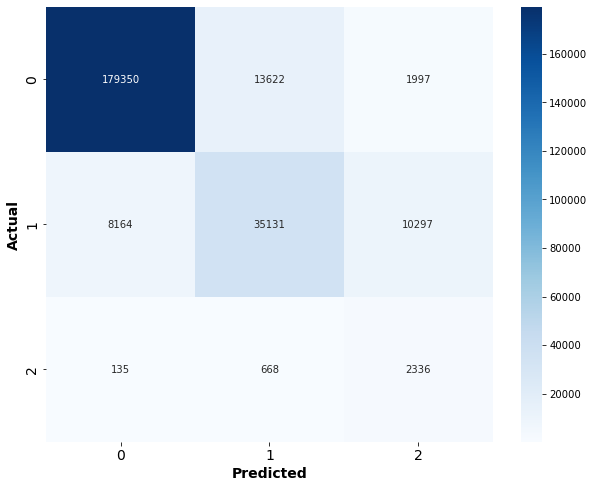
\includegraphics[width=0.73\linewidth]{Image/Confusionmatrix_LSTM.png}
    \caption{\centering Confusion Matrix for the LSTM model}
    \label{fig:Confusionmatrix_LSTM}
\end{figure}

\begin{figure}[H]
    \centering
    \includegraphics[width=0.89\linewidth]{Image/LSTM_loss.png}
    \caption{\centering Training and Validation Loss Over Epochs for the LSTM model}
    \label{fig:LSTM_LOSS}
\end{figure}

\noindent Figure \ref{fig:Confusionmatrix_LSTM} represents the confusion matrix for the final LSTM model. We note that the performance obtained for class 0 is excellent. Indeed, this matrix shows that for on-time flights, the model achieved a total of 179350 correct predictions, compared with only 15619 predictions misclassified as either class 1 or class 2. These results clearly demonstrate the robust performance of the LSTM model in predicting class 0. For the class of flight delays due to non-weather conditions, we observe that the LSTM model performs fairly well with 35131 correct predictions. The confusion matrix reveals that there is some confusion when predicting class 1, with 8164 instances wrongly classified as class 0 and 10297 instances misclassified as class 2. Concerning class 2, we can see that this model correctly predicted 2336 instances out of a total of 3139. Thus, this LSTM model misclassified 135 instances as class 0 and 668 instances as class 1. From all these observations, we deduce that while the LSTM model is clearly able to differentiate between on-time and delayed flights, it has some difficulty in capturing pertinent patterns in non-weather and weather delay data.

\noindent Figure \ref{fig:LSTM_LOSS} illustrates the training and validation loss over the number of epochs. This graph shows that the LSTM model converges well over the epochs. Indeed, we note that the training loss curve in blue decreases continuously until it slows down as the number of epochs increases. This means that this model is learning well during its training. We see that the validation loss curve in orange also follows a certain decreasing trend, although it is much less pronounced than the training loss curve. Thus, we can say there is no real sign of overfitting. Moreover, the validation loss curve does show several fluctuations. Such variations are likely a sign of some instability in the validation data.

\subsection{MultiLayer Perceptron}

\noindent In this subsection, we will discuss the evaluation of the performance of the MLP model. As explained in section \ref{hyperparameters_optimisation}, we adopted the same method as for the LSTM model, namely grid search. By using this approach, we were able to exhaustively test the following hyperparameters: learning rate, batch size, number of epochs, and the number of hidden nodes. Building on the results of all the configurations tested after the grid search, we will propose below a descriptive and critical analysis for the MLP model. This analysis will also include a discussion of the possible impact of the timing of weather data collection on the performance metrics adopted for the MLP model.

\setlength\LTleft{1.7cm}
\begin{longtable}{c c}
\caption{Tested hyperparameters in MLP model} \label{tab:MLP_hyperparameters} 
\\\hline
\textbf{Hyperparameters} & \textbf{Value} \\ \hline
\endfirsthead

\hline
\textbf{Hyperparameters} & \textbf{Value}  \\ \hline
&\\
\endhead

\hline \multicolumn{2}{r}{{Continued on next page}} \\ \hline
&\\
\endfoot

\hline
\endlastfoot
Learning rate & 0.001, 0.0001\\
Number of Epochs &  10, 20, 30, 50\\ 
Batch Size & 512, 1024\\ 
Number of hidden nodes & [128, 64, 32], [256, 128, 64], [512, 256, 128]\\
\end{longtable}

\noindent Table \ref{tab:MLP_hyperparameters} shows the values of the hyperparameters tested in the grid search for the MLP model. Each of the hyperparameter values listed in this table was chosen for a specific reason. For the learning rate, we followed the same approach as for the previous two models. Indeed, we used values of 0.001 and 0.0001 as they are regularly adopted in the optimisation of learning rates for ML/DL models \cite{Bengio2012}. Concerning the number of epochs, unlike the two previous models, we extended the range of the values tested: 10, 20, 30, and 50 epochs. Similar to the LNN and LSTM models, we also did not exceed 50 epochs to keep the execution time reasonable for grid search. Regarding batch size, unlike the LNN model, we used only two values: 512 and 1024. This choice helped to avoid making grid search too computationally intensive. We used 1024 because this value is fairly close to the one adopted in a previous research using the MLP model with a batch size of 1000. In addition, we selected 512 because, although it increases the execution time of the MLP model training, it also allows more precise convergence. For the number of hidden nodes, we took a different approach compared to the LNN and LSTM models. Indeed, we adopted a variable number of nodes for each layer of the model. This choice is driven by the fact that it reduces the complexity of the model by decreasing the number of nodes as we progress towards the output layer. It also reduces computational resource needs. Besides, we used a fixed number of 3 layers and a fixed dropout rate of 0.5 for all the configurations. This choice was made to avoid grid search being too resource-intensive and necessitating considerable execution time.

\noindent Similar to the LSTM model, we will present below the results obtained by the five best hyperparameter configurations for each timing of weather data collection. To define these different top 5, we selected them by taking into account all the performance metrics used.

\setlength\LTleft{+0.5cm}
\begin{longtable}{>{\centering\arraybackslash}p{2cm} p{12cm}}
\caption{\centering 5 Best hyperparameter configurations for the MLP model with weather data collected at 0h before flight departure} \label{tab:MLP_hyperparameters_config_0h} 
\\\hline
\textbf{S/No} & \textbf{Configurations} \\ \hline
\endfirsthead

\hline
\textbf{S/No} & \textbf{Configurations}  \\ \hline
&\\
\endhead

\hline \multicolumn{2}{r}{{Continued on next page}} \\ \hline
\endfoot

\hline
\endlastfoot
\\
1 & batch size=1024, number of epochs=50, number of layers=3, learning 

rate=0.001, dropout rate=0.5, number of hidden nodes=[512,256,218]\\
&\\
2 & batch size=1024, number of epochs=20, number of layers=3, learning 

rate=0.001, dropout rate=0.5, number of hidden nodes=[128, 64, 32]\\ 
&\\
3 & batch size=512, number of epochs=50, number of layers=3, learning 

rate=0.001, dropout rate=0.5, number of hidden nodes=[512, 256, 128]\\
&\\
4 & batch size=512, number of epochs=20, number of layers=3, learning 

rate=0.001, dropout rate=0.5, number of hidden nodes=[512, 256, 128]\\ 
&\\
5 & batch size=512, number of epochs=30, number of layers=3, learning 

rate=0.001, dropout rate=0.5, number of hidden nodes=[512, 256, 128]\\
&\\
\end{longtable}

\setlength\LTleft{1cm}
\begin{longtable}{ c ccc ccc ccc c}
\caption{\centering Performance metrics of the MLP model for the top 5 configurations with weather data collected at 0h before flight departure} \\
\toprule
\textbf{Config.} & \multicolumn{3}{c}{\textbf{Class 0}} & \multicolumn{3}{c}{\textbf{Class 1}} & \multicolumn{3}{c}{\textbf{Class 2}} & \textbf{Global} \\
               & Prec. & Rec. & F1  & Prec. & Rec. & F1   & Prec. & Rec. & F1  & Acc. \\
\midrule
\endfirsthead

\caption[]{(continued)} \\
\toprule
\textbf{Config.} & \multicolumn{3}{c}{\textbf{Class 0}} & \multicolumn{3}{c}{\textbf{Class 1}} & \multicolumn{3}{c}{\textbf{Class 2}} & \textbf{Global} \\
               & Prec. & Rec. & F1  & Prec. & Rec. & F1   & Prec. & Rec. & F1  & Acc. \\
\midrule
\endhead

\bottomrule
\endfoot

\bottomrule
\endlastfoot

1 & 0.96 & 0.92 & 0.94 & 0.71 & 0.67 & 0.69 & 0.17 & 0.74 & 0.27 & 86.31\% \\
2 & 0.95 & 0.94 & 0.95 & 0.75 & 0.61 & 0.67 & 0.16 & 0.74 & 0.26 & 86.96\% \\
3 & 0.96 & 0.91 & 0.94 & 0.71 & 0.68 & 0.69 & 0.16 & 0.74 & 0.26 & 86.18\% \\
4 & 0.96 & 0.92 & 0.94 & 0.72 & 0.67 & 0.69 & 0.16 & 0.74 & 0.26 & 86.11\% \\
5 & 0.96 & 0.92 & 0.94 & 0.72 & 0.66 & 0.69 & 0.15 & 0.76 & 0.25 & 85.94\% \\
\end{longtable}

\setlength\LTleft{+0.5cm}
\begin{longtable}{>{\centering\arraybackslash}p{2cm} p{12cm}}
\caption{\centering 5 Best hyperparameter configurations for the MLP model with weather data collected at 2h before flight departure} \label{tab:MLP_hyperparameters_config_2h} 
\\\hline
\textbf{S/No} & \textbf{Configurations} \\ \hline
\endfirsthead

\hline
\textbf{S/No} & \textbf{Configurations}  \\ \hline
&\\
\endhead

\hline \multicolumn{2}{r}{{Continued on next page}} \\ \hline

\endfoot

\hline
\endlastfoot
\\
1 & batch size=512, number of epochs=50, number of layers=3, learning 

rate=0.0001, dropout rate=0.5, number of hidden nodes=[512, 256, 128]\\ 
&\\
2 & batch size=512, number of epochs=50, number of layers=3, learning 

rate=0.001, dropout rate=0.5, number of hidden nodes=[512, 256, 128]\\
&\\
3 & batch size=512, number of epochs=50, number of layers=3, learning 

rate=0.001, dropout rate=0.5, number of hidden nodes=[256, 128, 64]\\
&\\
4 & batch size=512, number of epochs=50, number of layers=3, learning 

rate=0.001, dropout rate=0.5, number of hidden nodes=[512, 256, 128]\\ 
&\\
5 & batch size=512, number of epochs=30, number of layers=3, learning 

rate=0.001, dropout rate=0.5, number of hidden nodes=[512, 256, 128]\\
&\\
\end{longtable}

\setlength\LTleft{1cm}
\begin{longtable}{ c ccc ccc ccc c}
\caption{\centering Performance metrics of the MLP model for the top 5 configurations with weather data collected at 2h before flight departure} \\
\toprule
\textbf{Config.} & \multicolumn{3}{c}{\textbf{Class 0}} & \multicolumn{3}{c}{\textbf{Class 1}} & \multicolumn{3}{c}{\textbf{Class 2}} & \textbf{Global} \\
               & Prec. & Rec. & F1  & Prec. & Rec. & F1   & Prec. & Rec. & F1  & Acc. \\
\midrule
\endfirsthead

\caption[]{(continued)} \\
\toprule
\textbf{Config.} & \multicolumn{3}{c}{\textbf{Class 0}} & \multicolumn{3}{c}{\textbf{Class 1}} & \multicolumn{3}{c}{\textbf{Class 2}} & \textbf{Global} \\
               & Prec. & Rec. & F1  & Prec. & Rec. & F1   & Prec. & Rec. & F1  & Acc. \\
\midrule
\endhead

\bottomrule
\endfoot

\bottomrule
\endlastfoot

1 & 0.96 & 0.92 & 0.94 & 0.72 & 0.64 & 0.68 & 0.15 & 0.74 & 0.26 & 86.09\% \\
2 & 0.96 & 0.91 & 0.93 & 0.70 & 0.66 & 0.68 & 0.16 & 0.74 & 0.26 & 85.86\% \\
3 & 0.95 & 0.92 & 0.94 & 0.71 & 0.64 & 0.67 & 0.16 & 0.74 & 0.26 & 86.00\% \\
4 & 0.96 & 0.92 & 0.93 & 0.70 & 0.66 & 0.68 & 0.16 & 0.74 & 0.26 & 85.86\% \\
5 & 0.96 & 0.92 & 0.94 & 0.70 & 0.65 & 0.67 & 0.16 & 0.74 & 0.26 & 85.81\% \\
\end{longtable}

\setlength\LTleft{+0.5cm}
\begin{longtable}{>{\centering\arraybackslash}p{2cm} p{12cm}}
\caption{\centering 5 Best hyperparameter configurations for the MLP model with weather data collected at 4h before flight departure} \label{tab:MLP_hyperparameters_config_4h} 
\\\hline
\textbf{S/No} & \textbf{Configurations} \\ \hline
\endfirsthead

\hline
\textbf{S/No} & \textbf{Configurations}   \\ \hline
&\\
\endhead

\hline \multicolumn{2}{r}{{Continued on next page}} \\ \hline
\endfoot

\hline
\endlastfoot
&\\
1 & batch size=512, number of epochs=50, number of layers=3, learning 

rate=0.001, dropout rate=0.5, number of hidden nodes=[512, 256, 128]\\
&\\
2 & batch size=1024, number of epochs=50, number of layers=3, learning 

rate=0.001, dropout rate=0.5, number of hidden nodes=[512, 256, 128]\\
&\\
3 & batch size=512, number of epochs=10, number of layers=3, learning 

rate=0.001, dropout rate=0.5, number of hidden nodes=[512, 256, 128]\\ 
&\\
4 & batch size=1024, number of epochs=30, number of layers=3, learning 

rate=0.001, dropout rate=0.5, number of hidden nodes=[256, 128, 64]\\ 
&\\
5 & batch size=512, number of epochs=30, number of layers=3, learning 

rate=0.0001, dropout rate=0.5, number of hidden nodes=[256, 128, 64]\\
&\\
\end{longtable}

\setlength\LTleft{1cm}
\begin{longtable}{ c ccc ccc ccc c}
\caption{\centering Performance metrics of the MLP model for the top 5 configurations with weather data collected at 4h before flight departure} \\
\toprule
\textbf{Config.} & \multicolumn{3}{c}{\textbf{Class 0}} & \multicolumn{3}{c}{\textbf{Class 1}} & \multicolumn{3}{c}{\textbf{Class 2}} & \textbf{Global} \\
               & Prec. & Rec. & F1  & Prec. & Rec. & F1   & Prec. & Rec. & F1  & Acc. \\
\midrule
\endfirsthead

\caption[]{(continued)} \\
\toprule
\textbf{Config.} & \multicolumn{3}{c}{\textbf{Class 0}} & \multicolumn{3}{c}{\textbf{Class 1}} & \multicolumn{3}{c}{\textbf{Class 2}} & \textbf{Global} \\
               & Prec. & Rec. & F1  & Prec. & Rec. & F1   & Prec. & Rec. & F1  & Acc. \\
\midrule
\endhead

\bottomrule
\endfoot

\bottomrule
\endlastfoot

1 & 0.95 & 0.93 & 0.94 & 0.73 & 0.66 & 0.69 & 0.16 & 0.71 & 0.26 & 86.97\% \\
2 & 0.95 & 0.93 & 0.94 & 0.73 & 0.66 & 0.69 & 0.16 & 0.70 & 0.26 & 86.76\% \\
3 & 0.95 & 0.94 & 0.94 & 0.74 & 0.61 & 0.67 & 0.15 & 0.73 & 0.25 & 86.61\% \\
4 & 0.95 & 0.93 & 0.94 & 0.73 & 0.63 & 0.68 & 0.15 & 0.71 & 0.25 & 86.62\% \\
5 & 0.95 & 0.93 & 0.94 & 0.72 & 0.62 & 0.66 & 0.14 & 0.73 & 0.24 & 86.00\% \\
\end{longtable}

\setlength\LTleft{+0.5cm}
\begin{longtable}{>{\centering\arraybackslash}p{2cm} p{12cm}}
\caption{\centering 5 Best hyperparameter configurations for the MLP model with weather data collected at 8h before flight departure} \label{tab:MLP_hyperparameters_config_8h} 
\\\hline
\textbf{S/No} & \textbf{Configurations} \\ \hline
\endfirsthead

\hline
\textbf{S/No} & \textbf{Configurations}  \\ \hline
&\\
\endhead

\hline \multicolumn{2}{r}{{Continued on next page}} \\ \hline
\endfoot

\hline
\endlastfoot
\\
1 & batch size=1024, number of epochs=30, number of layers=3, learning 

rate=0.001, dropout rate=0.5, number of hidden nodes=[512, 256, 128]\\ 
&\\
2 & batch size=1024, number of epochs=50, number of layers=3, learning 

rate=0.001, dropout rate=0.5, number of hidden nodes=[128, 64, 32]\\
&\\
3 & batch size=1024, number of epochs=10, number of layers=3, learning 

rate=0.001, dropout rate=0.5, number of hidden nodes=[128, 64, 32]\\
&\\
4 & batch size=1024, number of epochs=50, number of layers=3, learning 

rate=0.0001, dropout rate=0.5, number of hidden nodes=[512, 256, 128]\\
&\\
5 & batch size=512, number of epochs=50, number of layers=3, learning 

rate=0.0001, dropout rate=0.5, number of hidden nodes=[512, 256, 128]\\ 
&\\
\end{longtable}

\setlength\LTleft{1cm}
\begin{longtable}{ c ccc ccc ccc c}
\caption{\centering Performance metrics of the MLP model for the top 5 configurations with weather data collected at 8h before flight departure} \\
\toprule
\textbf{Config.} & \multicolumn{3}{c}{\textbf{Class 0}} & \multicolumn{3}{c}{\textbf{Class 1}} & \multicolumn{3}{c}{\textbf{Class 2}} & \textbf{Global} \\
               & Prec. & Rec. & F1  & Prec. & Rec. & F1   & Prec. & Rec. & F1  & Acc. \\
\midrule
\endfirsthead

\caption[]{(continued)} \\
\toprule
\textbf{Config.} & \multicolumn{3}{c}{\textbf{Class 0}} & \multicolumn{3}{c}{\textbf{Class 1}} & \multicolumn{3}{c}{\textbf{Class 2}} & \textbf{Global} \\
               & Prec. & Rec. & F1  & Prec. & Rec. & F1   & Prec. & Rec. & F1  & Acc. \\
\midrule
\endhead

\bottomrule
\endfoot

\bottomrule
\endlastfoot

1 & 0.96 & 0.92 & 0.94 & 0.71 & 0.66 & 0.68 & 0.16 & 0.72 & 0.26 & 86.30\% \\
2 & 0.95 & 0.94 & 0.94 & 0.73 & 0.62 & 0.67 & 0.16 & 0.70 & 0.26 & 86.63\% \\
5 & 0.95 & 0.95 & 0.95 & 0.76 & 0.59 & 0.67 & 0.15 & 0.70 & 0.25 & 86.93\% \\
4 & 0.96 & 0.92 & 0.94 & 0.72 & 0.63 & 0.67 & 0.14 & 0.74 & 0.24 & 85.73\% \\
3 & 0.96 & 0.92 & 0.94 & 0.71 & 0.64 & 0.67 & 0.14 & 0.74 & 0.24 & 85.51\% \\
\end{longtable}

\setlength\LTleft{+0.5cm}
\begin{longtable}{>{\centering\arraybackslash}p{2cm} p{12cm}}
\caption{\centering 5 Best hyperparameter configurations for the MLP model with weather data collected at 16h before flight departure} \label{tab:MLP_hyperparameters_config_16h} 
\\\hline
\textbf{S/No} & \textbf{Configurations} \\ \hline
\endfirsthead

\hline
\textbf{S/No} & \textbf{Configurations} \\ \hline
&\\
\endhead

\hline \multicolumn{2}{r}{{Continued on next page}} \\ \hline
\endfoot

\hline
\endlastfoot
\\
1 & batch size=512, number of epochs=10, number of layers=3, learning 

rate=0.001, dropout rate=0.5, number of hidden nodes=[512, 256, 128]\\ 
&\\
2 & batch size=512, number of epochs=30, number of layers=3, learning 

rate=0.001, dropout rate=0.5, number of hidden nodes=[256, 128, 64]\\
&\\
3 & batch size=512, number of epochs=20, number of layers=3, learning 

rate=0.001, dropout rate=0.5, number of hidden nodes=[512, 256, 128]\\
&\\
4 & batch size=1024, number of epochs=50, number of layers=3, learning 

rate=0.001, dropout rate=0.5, number of hidden nodes=[256, 128, 64]\\
&\\
5 & batch size=512, number of epochs=50, number of layers=3, learning 

rate=0.001, dropout rate=0.5, number of hidden nodes=[128, 64, 32]\\ 
&\\
\end{longtable}

\setlength\LTleft{1cm}
\begin{longtable}{ c ccc ccc ccc c}
\caption{\centering Performance metrics of the MLP model for the top 5 configurations with weather data collected at 16h before flight departure} \\
\toprule
\textbf{Config.} & \multicolumn{3}{c}{\textbf{Class 0}} & \multicolumn{3}{c}{\textbf{Class 1}} & \multicolumn{3}{c}{\textbf{Class 2}} & \textbf{Global} \\
               & Prec. & Rec. & F1  & Prec. & Rec. & F1   & Prec. & Rec. & F1  & Acc. \\
\midrule
\endfirsthead

\caption[]{(continued)} \\
\toprule
\textbf{Config.} & \multicolumn{3}{c}{\textbf{Class 0}} & \multicolumn{3}{c}{\textbf{Class 1}} & \multicolumn{3}{c}{\textbf{Class 2}} & \textbf{Global} \\
               & Prec. & Rec. & F1  & Prec. & Rec. & F1   & Prec. & Rec. & F1  & Acc. \\
\midrule
\endhead

\bottomrule
\endfoot

\bottomrule
\endlastfoot

1 & 0.95 & 0.93 & 0.94 & 0.73 & 0.64 & 0.68 & 0.15 & 0.69 & 0.25 & 86.72\% \\
2 & 0.95 & 0.93 & 0.94 & 0.71 & 0.64 & 0.67 & 0.16 & 0.69 & 0.25 & 86.46\% \\
3 & 0.96 & 0.92 & 0.94 & 0.70 & 0.63 & 0.66 & 0.14 & 0.72 & 0.24 & 85.68\% \\
4 & 0.95 & 0.93 & 0.94 & 0.72 & 0.63 & 0.67 & 0.15 & 0.69 & 0.24 & 86.35\% \\
5 & 0.95 & 0.94 & 0.94 & 0.73 & 0.59 & 0.65 & 0.15 & 0.70 & 0.24 & 86.39\% \\
\end{longtable}

\setlength\LTleft{+0.5cm}
\begin{longtable}{>{\centering\arraybackslash}p{2cm} p{12cm}}
\caption{\centering 5 Best hyperparameter configurations for the MLP model with weather data collected at 24h before flight departure} \label{tab:MLP_hyperparameters_config_24h} 
\\\hline
\textbf{S/No} & \textbf{Configurations} \\ \hline
\endfirsthead

\hline
\textbf{S/No} & \textbf{Configurations}  \\ \hline
&\\
\endhead

\hline \multicolumn{2}{r}{{Continued on next page}} \\ \hline
\endfoot

\hline
\endlastfoot
\\
1 & batch size=1024, number of epochs=50, number of layers=3, learning 

rate=0.001, dropout rate=0.5, number of hidden nodes=[512, 256, 128]\\
&\\
2 & batch size=512, number of epochs=50, number of layers=3, learning 

rate=0.001, dropout rate=0.5, number of hidden nodes=[512, 256, 128]\\ 
&\\
3 & batch size=1024, number of epochs=20, number of layers=3, learning 

rate=0.001, dropout rate=0.5, number of hidden nodes=[512, 256, 128]\\
&\\
4 & batch size=1024, number of epochs=10, number of layers=3, learning 

rate=0.001, dropout rate=0.5, number of hidden nodes=[512, 256, 128]\\ 
&\\
5 & batch size=512, number of epochs=30, number of layers=3, learning 

rate=0.001, dropout rate=0.5, number of hidden nodes=[512, 256, 128]\\
&\\
\end{longtable}

\setlength\LTleft{1cm}
\begin{longtable}{ c ccc ccc ccc c}
\caption{\centering Performance metrics of the MLP model for the top 5 configurations with weather data collected at 24h before flight departure} \\
\toprule
\textbf{Config.} & \multicolumn{3}{c}{\textbf{Class 0}} & \multicolumn{3}{c}{\textbf{Class 1}} & \multicolumn{3}{c}{\textbf{Class 2}} & \textbf{Global} \\
               & Prec. & Rec. & F1  & Prec. & Rec. & F1   & Prec. & Rec. & F1  & Acc. \\
\midrule
\endfirsthead

\caption[]{(continued)} \\
\toprule
\textbf{Config.} & \multicolumn{3}{c}{\textbf{Class 0}} & \multicolumn{3}{c}{\textbf{Class 1}} & \multicolumn{3}{c}{\textbf{Class 2}} & \textbf{Global} \\
               & Prec. & Rec. & F1  & Prec. & Rec. & F1   & Prec. & Rec. & F1  & Acc. \\
\midrule
\endhead

\bottomrule
\endfoot

\bottomrule
\endlastfoot

1 & 0.95 & 0.93 & 0.94 & 0.74 & 0.64 & 0.69 & 0.15 & 0.70 & 0.25 & 86.68\% \\
2 & 0.95 & 0.93 & 0.94 & 0.74 & 0.63 & 0.68 & 0.15 & 0.70 & 0.25 & 86.72\% \\
3 & 0.95 & 0.93 & 0.94 & 0.74 & 0.64 & 0.68 & 0.15 & 0.69 & 0.25 & 86.77\% \\
4 & 0.95 & 0.94 & 0.95 & 0.76 & 0.59 & 0.66 & 0.14 & 0.71 & 0.24 & 86.70\% \\
5 & 0.95 & 0.93 & 0.94 & 0.72 & 0.63 & 0.67 & 0.14 & 0.71 & 0.23 & 86.05\% \\
\end{longtable}

\setlength\LTleft{-0.5cm}
\begin{longtable}{c p{13cm}}
\caption{\centering 5 Best hyperparameter configurations for the MLP model with weather data collected at 48h before flight departure} \label{tab:MLP_hyperparameters_config_48h} 
\\\hline
\textbf{S/No} & \textbf{Configurations} \\ \hline
\endfirsthead

\hline
\textbf{Hyperparameters} & \textbf{Value}  \\ \hline
&\\
\endhead

\hline \multicolumn{2}{r}{{Continued on next page}} \\ \hline
\endfoot

\hline
\endlastfoot
\\
1 & batch size=1024, number of epochs=30, number of layers=3, learning rate=0.001, dropout rate=0.5, number of hidden nodes=[256, 128, 64]\\
&\\
2 & batch size=512, number of epochs=30, number of layers=3, learning rate=0.001, dropout rate=0.5, number of hidden nodes=[512, 256, 128]\\ 
&\\
3 & batch size=1024, number of epochs=50, number of layers=3, learning rate=0.001, dropout rate=0.5, number of hidden nodes=[128, 64, 32]\\
&\\
4 & batch size=512, number of epochs=50, number of layers=3, learning rate=0.001, dropout rate=0.5, number of hidden nodes=[128, 64, 32]\\ 
&\\
5 & batch size=512, number of epochs=20, number of layers=3, learning rate=0.001, dropout rate=0.5, number of hidden nodes=[128, 64, 32]\\
&\\
\end{longtable}

\setlength\LTleft{1cm}
\begin{longtable}{ c ccc ccc ccc c}
\caption{\centering Performance metrics of the MLP model for the top 5 configurations with weather data collected at 48h before flight departure} \\
\toprule
\textbf{Config.} & \multicolumn{3}{c}{\textbf{Class 0}} & \multicolumn{3}{c}{\textbf{Class 1}} & \multicolumn{3}{c}{\textbf{Class 2}} & \textbf{Global} \\
               & Prec. & Rec. & F1  & Prec. & Rec. & F1   & Prec. & Rec. & F1  & Acc. \\
\midrule
\endfirsthead

\caption[]{(continued)} \\
\toprule
\textbf{Config.} & \multicolumn{3}{c}{\textbf{Class 0}} & \multicolumn{3}{c}{\textbf{Class 1}} & \multicolumn{3}{c}{\textbf{Class 2}} & \textbf{Global} \\
               & Prec. & Rec. & F1  & Prec. & Rec. & F1   & Prec. & Rec. & F1  & Acc. \\
\midrule
\endhead

\bottomrule
\endfoot

\bottomrule
\endlastfoot

1 & 0.95 & 0.93 & 0.94 & 0.73 & 0.61 & 0.67 & 0.14 & 0.69 & 0.23 & 86.37\%
\\
2 & 0.95 & 0.92 & 0.94 & 0.71 & 0.63 & 0.67 & 0.14 & 0.70 & 0.23 & 85.88\%
\\
3 & 0.95 & 0.94 & 0.94 & 0.72 & 0.61 & 0.66 & 0.14 & 0.68 & 0.23 & 86.34\%
\\
4 & 0.95 & 0.94 & 0.94 & 0.72 & 0.59 & 0.65 & 0.14 & 0.69 & 0.23 & 86.05\%
\\
5 & 0.94 & 0.95 & 0.95 & 0.77 & 0.56 & 0.65 & 0.14 & 0.69 & 0.23 & 86.73\%
\\
\end{longtable}

\noindent From all the results achieved for the MLP model, we note that the learning rate has a possible influence on the performance of this model. Indeed, we find that configurations with a learning rate of 0.001 generally perform better than those with a learning rate of 0.0001. This is demonstrated by the fact that the majority of optimal configurations have a learning rate of 0.001. For instance, in the case of weather data collected 0 hours before flight departure, we can see that all configurations in the top 5 use a learning rate of 0.001. These configurations achieve a maximum global accuracy of 86.96\%. In addition, we observe that, for weather data from 4 hours before departure, Configuration 1 with a learning rate of 0.001 obtains an F1-score of 0.69 for class 1 and 0.26 for class 2. In comparison, Configuration 5 with a learning rate of 0.0001 has only an F1-score of 0.66 for class 1 and 0.24 for class 2. Despite the difference being very small, it does show a trend where using a higher learning rate guarantees that this model converges more quickly and captures patterns in the data more effectively. Besides, we note that in some situations, configurations with a learning rate of 0.0001 can achieve better results than those with a learning rate of 0.001. For example, using data collected 2 hours before departure, the best configuration has a learning rate of 0.0001, producing a global accuracy of 86.09\%. Even so, in general, a learning rate of 0.001 does give a slightly better global performance of the MLP model. We can explain this trend by faster convergence and an increased ability to adjust weights during training. Thus, this allows a better capture of the patterns in weather data, especially beneficial for classes 1 and 2.

\noindent In addition, we also note an influence of the number of epochs on the performance of the MLP model. From all the tests carried out on four different numbers of epochs, we observe that the configurations most represented in the various top 5 are those with a high number of epochs, particularly those with 50 epochs. In general, a higher number of epochs tends to improve the overall accuracy of metric performance, even though this is not always linear. For example, for weather data from 2 hours before departure, we observe that configurations with 50 epochs are present in the majority of this top 5. These configurations achieve a maximum global accuracy of 86.09\%. Moreover, using weather data collected 0 hours before departure, we find that Configuration 1 with 50 epochs achieves an F1-score of 0.69 for class 1 and 0.27 for class 2. In contrast, Configuration 2 for the same data reaches an F1-score of 0.67 for class 1 and 0.26 for class 2. However, it is possible to obtain interesting results with fewer epochs. For example, with weather data taken 16 hours before departure, the best configuration uses 10 epochs, achieving F1-scores of 0.68 and 0.25 for classes 1 and 2 respectively. This can be explained by the fact that the other hyperparameters are well optimised. Thus, while configurations with a larger number of epochs seem to provide better performance and quite high metric performance scores, there are some cases where configurations with fewer epochs can be just as effective.

\noindent Moreover, the results obtained on the performance of the MLP model indicate some interesting trends for batch size. Indeed, we note that for the configurations tested, the global performance varies relatively slightly regardless of batch size. To some extent, we observe important nuances. Overall, configurations with a batch size of 512 show a slight performance advantage over those with a batch size of 1024. Indeed, out of all the best configurations tested across the different data collection timings, we find that the majority use a batch size of 512. For example, using weather data 2 hours before departure, we notice that all configurations in the top 5 use a batch size of 512, achieving a maximum global accuracy of 86.09\%. This tendency can also be seen for other timings, albeit to a lesser extent. For example, for weather data from 4 hours before departure, we notice that Configuration 1 with a batch size of 512 reaches a recall of 0.66 for class 1 and a global accuracy of 86.97\%, compared with a recall of 0.63 for class 1 and a global accuracy of 86.62\% for Configuration 4 having a batch size of 1024. These findings could mean that a batch size of 512 provides better generalisation capability because of the more frequent updating of weights. We also note that this difference in performance is very subtle and not totally consistent. In some situations, batch sizes of 1024 can offer similar or even slightly better performance. For example, for weather data taken 8 hours before departure, Configuration 1 using a batch size of 1024 shows an F1-score of 0.68 for class 1 and 0.26 for class 2. In comparison, Configuration 5 with a batch size of 512 shows an F1-score of 0.67 and 0.24 for class 1 and 2 respectively. Thus, even though batch sizes of 512 show a small tendency to offer better overall performance, the impact of this hyperparameter on the results of the MLP model remains moderate. Such impact may vary depending on the other hyperparameters and the timing of weather data collection.

\noindent Besides, we find an impact of the number of hidden nodes on the performance of the MLP model. We observe a general trend indicating that configurations with a hidden node structure of [512, 256, 128] show better performance than those with less complex structures. Indeed, these configurations with a complex node structure frequently appear among the best configurations for the different collection timings, namely more than 60\% of the time. For example, using data collected 4 hours before flight departure, Configuration 1 with a node structure of [512, 256, 128] achieves a global accuracy of 86.97\%. In comparison, Configuration 5 with a less complex node structure of [256, 128, 64] has a global accuracy of 86.00\%. In addition, configurations with such complex structures are also effective for other timings. For example, at 24 hours, Configuration 1 with a node structure of [512, 256, 128] shows an F1-score of 0.69 for class 1 and 0.25 for class 2 as well as a global accuracy of 86.68\%. However, the impact of the number of nodes is not uniform. Indeed, there are some situations where configurations with fewer nodes perform just as well, or even better. For example, for weather data from 48 hours before, Configuration 1 with [256, 128, 64] nodes achieves 86.37\% accuracy, compared with 85.88\% for Configuration 2 with [512, 256, 128] nodes. Such variability implies a complex interaction between the number of nodes, the other hyperparameters and the timing of the weather data. Thus, we observe that configurations with more nodes generally seem to perform better on more recent data. This can be explained by the fact that complex configurations have the capacity to capture more complex patterns. However, with weather data collected well in advance of flight departure, simpler configurations can sometimes offer comparable or even better results.

\noindent Finally, the various tests carried out to study the performance of the MLP model using different configurations show the strong influence of the timing of weather data collection on its performance. We note a general trend where data collected closer to the time of flight departure leads to better performance. For example, for weather data collected 0 hours before departure, Configuration 1 obtains F1-scores of 0.69 and 0.27 for classes 1 and 2 respectively. For weather data collected 2 hours before departure, Configuration 1 achieves an F1-score of 0.68 for class 1 and 0.26 for class 2. We find that the best configurations for each timing of weather data collection have fairly similar scores for these performance metrics, except for weather data collected 48 hours before departure. This decrease strongly indicates that the use of weather data close to flight departure plays an important role in the accuracy of the predictions. Moreover, we observe that for class 2, the F1-score drops from 0.27 for weather data collected 0 hours before departure to 0.23 for weather data collected 48 hours before departure. This shows that the model has difficulty predicting flight delays due to weather conditions with older weather data. This appears logical, as weather conditions captured 48 hours before a flight are unlikely to stay the same at the time of departure. Nevertheless, the relative stability of performance up to 24 hours before departure implies that the MLP model is capable of capturing pertinent meteorological patterns even with data collected a day in advance.

\noindent Based on the critical and descriptive analysis of the results, we were able to identify the best hyperparameter configuration for the MLP model:
\begin{multicols}{2}
    \begin{itemize}
        \item Learning rate = 0.001
        \item Number of epochs = 50
        \item Number of layers = 3
        \item Number of hidden nodes = [512, 256, 128]
    \end{itemize}
    \begin{itemize}
         \item Timing of weather data collection: 0h
         \item Dropout rate  = 0.5
         \item Batch size = 1024
         \item[\hspace{0pt}]
    \end{itemize}
\end{multicols}

\noindent This represents Configuration 1 with weather data collected 0 hours before departure. This choice was made to the detriment of other interesting configurations, such as Configuration 1 with weather data collected 4 hours before departure. Indeed, the selected configuration showed a fairly high global accuracy, with the best F1-scores obtained for classes 1 and 2 among all the configurations tested. In addition, the precision obtained for class 2 is particularly remarkable for this optimum configuration. Below, we will concentrate on the performance of the best MLP model chosen. The purpose is to analyse its performance from different angles. To achieve this, we will mainly examine the training and validation loss, as well as the confusion matrix.

\begin{figure}[H]
    \centering
    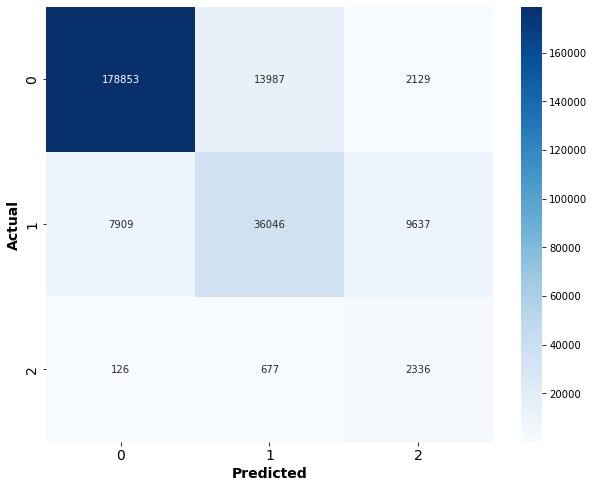
\includegraphics[width=0.75\linewidth]{Image/Confusionmatrix_MLP.png}
    \caption{\centering Confusion Matrix for the MLP model}
    \label{fig:Confusionmatrix_MLP}
\end{figure}

\begin{figure}[H]
    \centering
    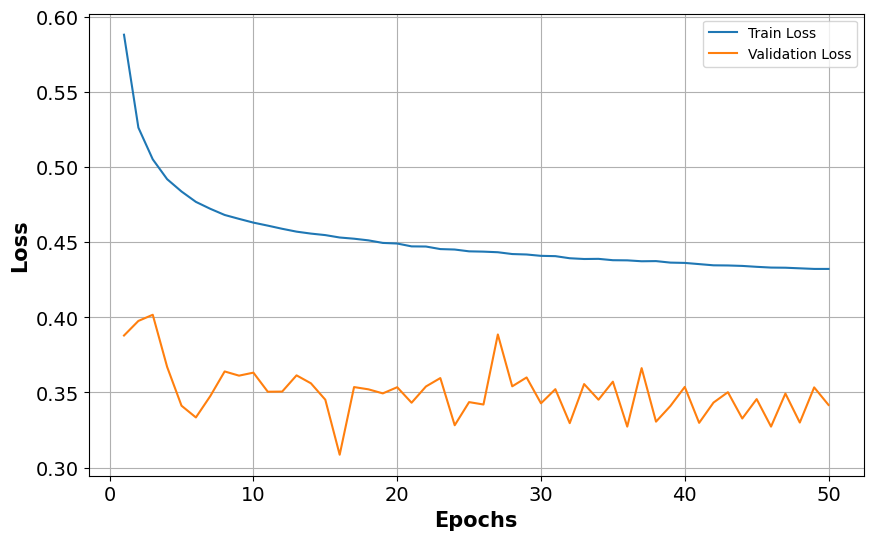
\includegraphics[width=\linewidth]{Image/MLP_loss.png}
    \caption{\centering Training and Validation Loss Over Epochs for the MLP model}
    \label{fig:MLP_LOSS}
\end{figure}

\noindent Figure \ref{fig:Confusionmatrix_MLP} shows the confusion matrix of the final MLP model. This matrix demonstrates an overall good performance for classifying class 0, namely on-time flights. Indeed, the final MLP model achieves correct predictions for class 0 with 178853 instances and has a relatively low error rate with only 13987 instances misclassified as class 1 and 2129 as class 2. Regarding class 1, the MLP model shows a fairly good classification capacity with 36046 correct predictions. However, the model misclassified 7909 instances as class 0 and 9637 as class 2. Finally, class 2 performed less well, with only 2336 correct predictions, compared with 677 misclassified predictions in class 1 and 126 in class 0. These results confirm that the model has some difficulty in clearly distinguishing whether the flight is delayed due to non-weather conditions or due to weather conditions. Indeed, too many flights are wrongly classified as delayed due to weather conditions. However, it is better to wrongly predict class 2 than to under-predict this class.

\noindent Figure \ref{fig:MLP_LOSS} represents the training and validation loss for the MLP model. This graph shows that the training loss curve in blue tends to decrease over the epochs. This curve also appears to converge as the number of epochs increases. Such observations indicate that the model continues to learn efficiently and to adjust to the data through weight updates. Concerning the validation loss in orange, it displays much higher variability. While this curve seems to decrease very slightly, it fluctuates around a certain value after 10 epochs. The stability may indicate that the MLP model is reaching a point of overfitting, as it continues to learn from training data with no obvious improvement in validation data. This stability of the validation loss also shows that the model achieves a good compromise between bias and variance. These fluctuations could be due to the imbalances in validation data.

\subsection{Model Comparison}

\noindent Below, we will compare in detail the performance of the best LNN, LSTM and MLP models. The main purpose of this comparison is to identify the best performing DL model developed among these three by using several performance metrics. This comparative, constructive and critical analysis will enable us to highlight the strengths and weaknesses of each approach from different points of view.

\setlength\LTleft{1cm}
\begin{longtable}{ c ccc ccc ccc c}
\caption{\centering Summary table of the performance of the best LNN, LSTM and MLP models} 
\label{comparison1}
\\
\toprule
\textbf{Model} & \multicolumn{3}{c}{\textbf{Class 0}} & \multicolumn{3}{c}{\textbf{Class 1}} & \multicolumn{3}{c}{\textbf{Class 2}} & \multicolumn{1}{c}{\textbf{Global}} \\
               & Prec. & Rec. & F1  & Prec. & Rec. & F1   & Prec. & Rec. & F1  & Acc. \\
\midrule
\endfirsthead

\caption[]{(continued)} \\
\toprule
\textbf{Model} & \multicolumn{3}{c}{\textbf{Class 0}} & \multicolumn{3}{c}{\textbf{Class 1}} & \multicolumn{3}{c}{\textbf{Class 2}} & \multicolumn{1}{c}{\textbf{Global}} \\
               & Prec. & Rec. & F1  & Prec. & Rec. & F1   & Prec. & Rec. & F1  & Acc. \\
\midrule
\endhead

\bottomrule
\endfoot

\bottomrule
\endlastfoot

LNN & 0.96  & 0.92 & 0.94 & 0.71  & 0.70 & 0.71  & 0.18  & 0.67 & 0.29 & 86.82\% 
\\
LSTM & 0.96 & 0.92 & 0.94 & 0.71 & 0.66 & 0.68 & 0.16 & 0.74 & 0.26 & 86.14\%
\\
MLP & 0.96 & 0.92 & 0.94 & 0.71 & 0.67 & 0.69 & 0.17 & 0.74 & 0.27 & 86.31\% 
\\
\end{longtable}

\noindent Table \ref{comparison1} summarises the performance of the best LNN, LSTM, and MLP models. It is important to note that all three models use weather data collected 0 hours before flight departure. This suggests that to optimise the chances of accurately predicting flight arrival weather delays, it is better to use the most recent weather data prior to departure.

\noindent The analysis of the performance of these models reveals similarities and subtle differences. We note that these DL models show quite similar results in terms of global accuracy. The LNN model obtains a score of 86.82\%, slightly better than the MLP and LSTM models, which achieve scores of 86.31\% and 86.14\% respectively. This small variation indicates that these models reach a comparable level of performance from an overall point of view. In addition, we find that a similarity emerges in the performance of the three models for class 0. All these models achieve the same scores on the three performance metrics adopted for this class. Such results show that the three models have an excellent ability to identify on-time flights. Regardless of the model chosen, performance for class 0 remains high.

\noindent Moreover, we find that the differences in performance are more apparent and marked for the other two classes. For class 1, the LNN is superior to the other two models with an F1-score of 0.71, compared with 0.69 for the MLP and 0.68 for the LSTM. Similarly, we observe that the LNN shows better recall scores for class 1 compared with the other models. This means that the LNN model has a higher capacity to correctly identify non-weather delays. Concerning class 2, namely delays due to weather conditions, the results are quite interesting. Despite the LNN model having the highest F1-score, we can see that the two remaining models exhibit better recall with 0.74 compared to 0.67 for the LNN. This implies that these two models will tend to predict more frequently that the flight will be classified as class 2, even if it comes at the cost of slightly lower precision.

\setlength\LTleft{4cm}
\begin{longtable}{ c cc} 
\caption{\centering Execution Time in Training and Testing for LNN, LSTM and MLP models} 
\label{comparison2}
\\
\toprule
\textbf{Model} & \multicolumn{2}{c}{\textbf{Execution Time}}\\
               & Training Time (s) & Testing Time (s)\\
\midrule
\endfirsthead

\caption[]{(continued)} \\
\toprule
\textbf{Model} & \multicolumn{2}{c}{\textbf{Execution Time}}\\
               & Train (s) & Test (s)\\
\midrule
\endhead

\bottomrule
\endfoot

\bottomrule
\endlastfoot

LNN & 21093.2756 & 29.4773
\\
LSTM & 2853.6685 & 8.3534
\\
MLP & 1014.9677 & 3.1419
\\
\end{longtable}

\noindent Table \ref{comparison2} provides some interesting insights into the computational efficiency of the three DL models. In terms of model training, we note that the MLP model clearly stands out by showing the best result among these models. Indeed, we see that its training time is around 1015 seconds. Its training time is relatively short compared with the other two models. Such finding highlights the good performance of this MLP model in terms of computational efficiency. Indeed, the LSTM model requires more than twice as much time with a training time of 2853 seconds. The LNN model obtains the worst result with a time of 21093 seconds. This performance of the LNN model reflects its slowness during training.

\noindent In terms of model evaluation, we can see that all these models show fairly encouraging results with relatively short testing times. Similar to training times, we find the same trend in the performance of the models in terms of computational efficiency. Indeed, the MLP model once again performs very well, with a testing time of 3.1419 seconds. In comparison, the LSTM model has a testing time of 8.3534 seconds and the LNN model a testing time of 29.4773 seconds.

\noindent It is useful to question the relevance of training execution time as a metric for evaluating model performance. Indeed, in numerous real-time prediction contexts, the use of pretrained models is commonly considered. Such approach is interesting because it can considerably reduce the computational costs related to training. As a result, this performance metric becomes less relevant for performance evaluation. The use of a pretrained model is quite advantageous for the LNN since its training time is notably long. By using the pretrained model approach, the LNN model could overcome this disadvantage and deliver performance closer to that of the other two models in terms of computational efficiency.

\noindent From all these observations of the performance of the models, we can draw the following conclusions: 

\begin{itemize}
    \item The LNN model shows the best performance for prediction accuracy. It also delivers an interesting balance between classes 1 and 2. In addition, its F1-score for class 2 is very beneficial for predicting flight weather delays. Although acceptable, its testing time remains the longest of the three models. 
    \item The MLP model delivers an acceptable compromise between the prediction performance and the execution speed. Its prediction performance is slightly lower compared to the LNN model, especially for classes 1 and 2. Its testing time is the shortest among the three models. This may be a decisive factor.
    \item The LSTM model shows the poorest performance in terms of prediction. Indeed, the results achieved for classes 1 and 2 are slightly lower than those of the MLP model. Its testing time, while longer in comparison with the MLP model, is still within an acceptable range.
\end{itemize}

\noindent Taking into account the use of the best model for real-time applications, we decided to choose the LNN model. After training, this DL model can be saved and deployed directly for predictions. This resolves the main issue with the LNN model with its training time. We prioritised prediction accuracy over computational efficiency. Such decision was driven by the desire to maximise the accuracy of the model for class 2, which is very difficult to predict. Moreover, even though the MLP model delivers solid advantages, the difference in testing time is not sufficiently important to justify its choice over the LNN model. By saving the LNN after training, we guarantee that future predictions can be made relatively quickly while still having good accuracy.

\noindent To extend this analysis, we will now compare the performance of the best model determined previously with two other models from past research in this field. This comparison is necessary to rigorously evaluate the possible improvements made by the LNN model developed in this thesis compared to previous work. The two models from past research include a DL model and an ML model. Using them, we can evaluate the performance of the best model from different angles. This comparative evaluation will help us determine whether the proposed model represents a real advance over existing techniques. In this way, we will be able to draw some conclusions about the contributions of the work done in this thesis to the state of the art in the area.

\setlength\LTleft{1cm}
\begin{longtable}{c ccc ccc ccc c}
\caption{Comparison of the performance of the best model with two models from previous research}
\label{comparison3}
\\
\hline
\textbf{Model} & \multicolumn{3}{c}{\textbf{Class 0}} & \multicolumn{3}{c}{\textbf{Class 1}} & \multicolumn{3}{c}{\textbf{Class 2}} & \textbf{Global} \\
               & Prec. & Rec. & F1  & Prec. & Rec. & F1   & Prec. & Rec. & F1  & Acc. \\
\hline
\endfirsthead

\caption[]{(continued)}\\
\hline
\textbf{Model} & \multicolumn{3}{c}{\textbf{Class 0}} & \multicolumn{3}{c}{\textbf{Class 1}} & \multicolumn{3}{c}{\textbf{Class 2}} & \textbf{Global} \\
               & Prec. & Rec. & F1  & Prec. & Rec. & F1   & Prec. & Rec. & F1  & Acc. \\
\hline
\endhead

\hline
\endfoot

\hline
\endlastfoot

LNN & 0.96  & 0.92 & 0.94 & 0.71  & 0.70 & 0.71  & 0.18  & 0.67 & 0.29 & 86.82\%\\
\hline
\multirow{2}{*}{\textbf{Model}} & \multicolumn{3}{c}{\textbf{Class 0}} & \multicolumn{6}{c}{\textbf{Class 1 (Combined)}} & \textbf{Global} \\
               & Prec. & Rec. & F1  & \multicolumn{2}{c}{Prec.} & \multicolumn{2}{c}{Rec.} & \multicolumn{2}{c}{F1} & Acc. \\
\hline
LSTM \cite{kim} & 0.83 & 0.88 & 0.86 & \multicolumn{2}{c}{0.88} & \multicolumn{2}{c}{0.82} & \multicolumn{2}{c}{0.85} & 85.2\% \\
RF \cite{kim} & 0.84 & 0.86 & 0.85 & \multicolumn{2}{c}{0.85} & \multicolumn{2}{c}{0.82} & \multicolumn{2}{c}{0.84} & 84.3\% \\
\end{longtable}

\noindent Table \ref{comparison3} shows a performance comparison between the LNN model developed in this thesis and two models from the study by S. Kim and E. Park \cite{kim}: a LSTM model and a RF model. We selected these two models for many reasons. Firstly, that previous study was carried out in 2024, which enables a comparison with recent results. In addition, that study uses data quite similar to those employed in this thesis, from the same source and relating to JFK airport. The only difference is that the LNN model was trained with two extra years of data, whereas the models in the study also incorporated data from the COVID-19 period. That previous study also tested their models with datasets of weather data collected at different times before the flight. It is important to note a major difference in the structure of the results. The LNN model distinguishes three classes, whereas the LSTM and RF models only identify two. The LNN model separates the category of delays into two: delays due to non-weather conditions with class 1 and those due to weather conditions with class 2. In contrast, the LSTM and RF models predict only flight delays with class 1, independent of their cause. This difference in the structure of the classification makes direct comparison more complex but it does offer some interesting insights. Besides, we have not taken into account the metrics related to training and testing times. This decision was made because the LSTM and RF models did not use the same computational resources as the LNN model.

\noindent In terms of global accuracy, we find that the LNN model developed in this thesis displays an impressive score compared to those in the study by S. Kim and E. Park \cite{kim}. Indeed, the LNN model performs well with an accuracy of 86.82\%, slightly better than the LSTM model at 85.2\% and the RF model at 84.3\%. Even though this difference is quite small, it does indicate a certain improvement in the global performance of the LNN model compared with these previous approaches.

\noindent For the on-time flight class, we note that the LNN model achieves excellent results compared with the other two models, LSTM and RF. The LNN model achieves very high scores for precision, recall, and F1-score with 0.96, 0.92, and 0.94 respectively. In comparison, the LSTM and RF models show lower scores, between 0.83 and 0.88 for the same performance metrics. This clearly indicates that the LNN model is more effective at predicting on-time flights than the two models from the previous study. This improvement underlines one of the benefits of adopting the LNN model.

\noindent Besides, the comparison of the other classes is much more challenging because of the different structure of the results between the LNN model and the RF and LSTM models. We note that, for predicting flight delays, the LSTM and RF models perform quite well with F1-scores of 0.85 and 0.84 respectively. The LNN model obtains an F1-score of 0.71 for flight delays due to non-weather conditions and 0.29 for delays due to weather conditions. This reveals a marked difference between the ability of the models in the previous study and the LNN model in this thesis to predict delays. It is difficult to say whether the LNN model underperforms compared to the other two models, as they do not specifically distinguish between weather and non-weather delays. We may explain this difference by the fact that differentiating weather and non-weather delays is probably a more complex task than simply classifying delays.

\noindent To have a direct comparison for delay prediction, we followed the following approach. Using the confusion matrix in Figure 4.2, we merged the predictions from classes 1 and 2 into a single class. Then, we recomputed the values of each performance metric. With this approach, the LNN model obtains 0.86 for precision, 0.75 for recall, and 0.80 for F1-score. These results demonstrate that when classes 1 and 2 are merged to evaluate the overall performance on flight delays of the LNN model, the scores are slightly lower than those of the other two models for some metrics. Despite this drop in performance on the delay classes, the LNN model delivers a major advantage in terms of interpretability and usefulness. Indeed, the ability to distinguish between types of delay may be important.

\noindent From all these observations, we can see that the LNN model developed in this thesis provides added value in the field of flight delay prediction. The LNN model is distinguished by better global accuracy and superior performance in predicting class 0, while providing the ability to differentiate delays into two types. With the two delay classes of the LNN model, we can obtain more detailed predictions as well as a better insight into the factors influencing flight delays. The LNN model has some limitations with a few difficulties in predicting flight delays compared with the previous model. In addition, these limitations also reflect an imbalance in the performance of the LNN model between the prediction of delay classes and class 0. These limitations can be explained by numerous factors. Firstly, weather data is often subject to a degree of uncertainty, which can affect the accuracy of weather-related delay predictions. Moreover, many factors other than weather conditions are likely to cause flight delays. These factors may not be correctly reflected in the data used for training.

\chapter{Conclusions \& Future Works}

\section{Overall}

\noindent This thesis focused on the implementation and evaluation of DL models for the prediction of flight delays with a particular emphasis on those due to weather conditions. The principal aim was to introduce a new DL approach, previously unseen in this field, via the development of the LNN model. Besides, this thesis is notable for its in-depth analysis of delays, making it possible to differentiate between those caused by weather conditions and those caused by some other factors.

\noindent We explored various NN architectures, including LNN, LSTM, and MLP models. By adopting a rigorous data processing methodology, from handling missing values to managing data imbalance with the SMOTE algorithm, we were able to provide each model with high-quality data for training. The models were optimised using established methods, such as grid search and the trial-and-error approach, to identify the configurations offering the best performance.

\noindent The results obtained showed that the LNN model performs slightly better overall than the other two models tested in this thesis, namely the LSTM and MLP models. In addition, the LNN model also demonstrated superior performance in certain metrics compared to the LSTM and RF models used in a previous study. In particular, we were able to improve certain aspects of flight delay prediction, notably in terms of global accuracy as well as precision, recall, and F1-score for on-time flights. These improvements demonstrate the effectiveness of the LNN model and its ability to surpass previous approaches in this area. This thesis has also demonstrated that the use of weather data collected close to the departure time improves the global accuracy of predicting arrival delays. By distinguishing delays according to their causes, this thesis brings additional depth to the prediction of delays.

\noindent However, there are some limitations to this thesis. Although the LNN model performed well overall, predicting weather delays remains a challenge. The results for these delays obtained by the LNN model demonstrated considerably lower scores compared to those achieved for the other classes. As a consequence, there is a clear need for improvement in this specific class. In addition, the LNN model is very demanding with regard to computational resources. This is reflected with longer training times than other approaches. Finally, because of the integration of weather data into the model, a certain degree of uncertainty may be present in the data, negatively affecting the robustness of the model.

\noindent Overall, the LNN model delivers a solid foundation for flight delay prediction. It creates new ways for improving prediction accuracy and even optimising flight operations.

\section{Future Works}

\noindent Potential directions for future work and possible improvements have been identified based on the observations, results, and limitations identified in this thesis.

\noindent Firstly, the optimisation of hyperparameters can be enhanced. To achieve this, we could continue to test more configurations for the LNN model by varying the dropout rate, for example, or extend the sets of values of the hyperparameters tested during the grid search for the LSTM and MLP models. We could also add a hyperparameter representing the SMOTE imbalance ratio and vary it to see if this improves prediction accuracy. Besides, we could also attempt to simplify the optimisation of the LNN model by moving from a trial-and-error approach to the grid search method. To do this, we will need to find some ways to reduce the high demand for resources of this model.

\noindent Secondly, to improve the predictions, especially for class 2, it could be interesting to try and collect weather data from the itineraries of each flight. Indeed, arrival delays can also be influenced by weather conditions encountered during the flight or just before the flight arrival.

\noindent Besides, to improve the evaluation of the models and their generalisation, it may be relevant to evaluate the models with flight and weather data from another airport. In this way, the idea would be to check whether the models developed can be used in other airports while retaining consistency in the predictions.

\noindent Moreover, to extend the work of this thesis, it can be useful to take into account cancelled flights and consider them as a type of infinite delay. Thus, when predicting with the models, if they predict that the flight is delayed, whether due to weather conditions or not, they will also predict whether the flight is cancelled or not. To achieve this, we will need to add a second output layer for the models which will only deal with the prediction of cancelled flights.

\noindent Finally, it would be relevant to study the prediction of flight delays due to some other factors. To achieve this, it will be necessary to analyse and integrate extra data associated, for instance, with operational or technical problems to predict air carrier delays. By extending flight delay prediction to include other causes alongside weather delays, the utility of the model can be improved, thus making it a more robust tool.

% This is where we include references and appendices
%\bibliographystyle{abbrvnat}
\bibliographystyle{unsrt} % "unsrt" 
\bibliography{LaTeX,ReportBibliography}

\appendix
\chapter{CURES}
\vspace{0.2cm}
\begin{figure}[H]
    
\includepdf[pages=-, scale=0.9, pagecommand={\thispagestyle{fancy}}]{Letter.pdf}
\end{figure}

\clearpage
\chapter{Source Code}

\begin{figure}[H]
    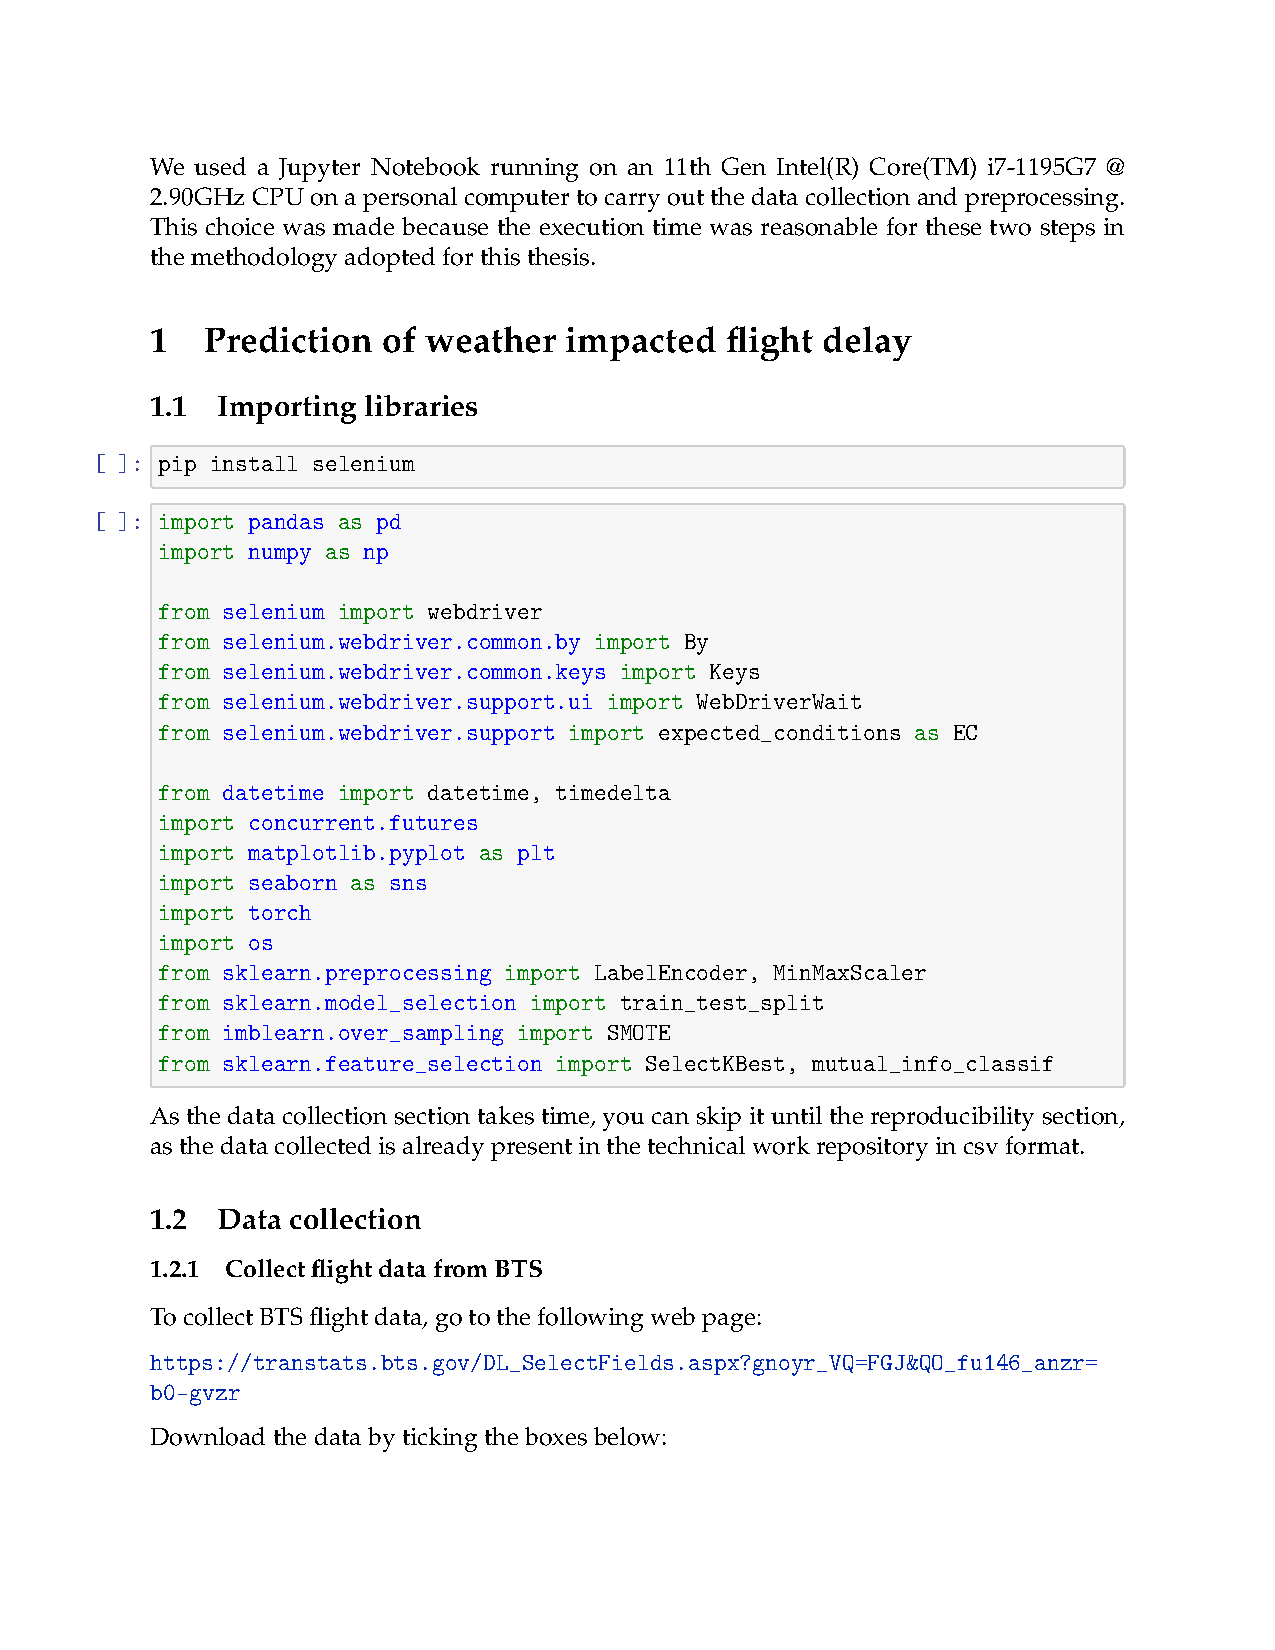
\includepdf[pages=1, scale=0.9, pagecommand={\thispagestyle{fancy}}]{Chandrakumar_s419255_CodingFile_MScCSTE.pdf}
\end{figure}


\includepdf[pages=2-, scale=0.9, pagecommand={\thispagestyle{fancy}}]{Chandrakumar_s419255_CodingFile_MScCSTE.pdf}

\end{document}

